\chapter{Détection des anomalies dans les délais d'un lien}\label{chap:algorith-detection}

\section{Introduction}
Dans le présent chapitre, nous présentons l'outil de détection des anomalies dans les délais d'un lien. Cet outil a été  conçu dans le cadre du travail \cite{DBLP:journals/corr/FontugneAPB16}  de  Fontugne et al.. Nous avons choisi de réutiliser ce travail qui se base sur les traceroutes collectés par les sondes, et ce en vue d'évaluer son implémentation avec quelques technologies  Big Data.  

\section{Présentation générale}

Dans leur travail \cite{DBLP:journals/corr/FontugneAPB16}, Fontugne et al. ont exploité la grande répartition  des sondes  dans le monde afin d'étudier le délai des liens topologiques sur les réseaux informatiques et de tracer son évolution; c'est le délai entre deux routeurs adjacents sur Internet.

L'idée de ce travail est de collecter les résultats des requêtes traceroute effectuées par les sondes, d'en déterminer une valeur de référence du délai du lien en question sur base de  son historique, et ensuite de comparer la référence avec la valeur courante.  Cette référence est mise à jour au fur et au mesure de l'analyse de nouveaux traceroutes. 
La comparaison de la référence avec la valeur courante ne se déclenche que lorsque cette  référence est assez représentable de l'état réel\footnote{Avec une probabilité de $95\%$.} du lien.

Le travail \cite{DBLP:journals/corr/FontugneAPB16} de  Fontugne et al.  comprend trois méthodes. Nous allons travailler sur la méthode ayant pour objectif la détection des changements des délais que subissent les liens intermédiaires dans les traceroutes.

\section{Pourquoi analyser les délais des liens  ?}

%Il existe un bon nombre de sujets à traiter en exploitant les données collectées par les sondes Atlas. Quelques exemples de sujets ont été déjà présentés dans la section \ref{use-cases-atlas}. Notre choix de reprendre le travail de Fontugne et al. \cite{DBLP:journals/corr/FontugneAPB16} a été fait après avoir parcouru un ensemble de travaux basés sur le projet  RIPE Atlas. 

Pour certains travaux, il n'était pas possible  de les reprendre suite au manque de détails et de l'accès à  certaines ressources réseaux utilisées dans ces travaux \footnote{Par exemple, les informations du peering entre les Systèmes Autonomes, la géolocalisation des adresses IP, etc.}. Par exemple, afin d'étudier la censure dans un pays donné, il faut être au courant des spécificités de ce pays, les circonstances politiques et sociales, les opposants,  etc.  Un autre exemple concerne le sujet de la détection des détours du trafic local dans un pays.  Anant Shah  et al. ont travaillé sur la détection des détours, ils ont présenté dans  \cite{anant-shah} les contraintes relatives à ce sujet: la difficulté d'avoir une géolocalisation exacte d'une adresse IP d'une part et l'absence des informations de peering entre les ASs d'autre part. Ces dernières peuvent changer complètement les conclusions finales. 

Le travail sur lequel nous nous basons \cite{DBLP:journals/corr/FontugneAPB16} pour l'évaluation de quelques technologies Big Data s'inscrit dans les travaux traitant les performances des réseaux informatiques. Dans la suite de ce document, ce travail est appelé  travail de référence.  Ce travail a été choisi comme référence pour plusieurs raisons:



\paragraph{Les données utilisées}  Les auteurs de ce travail ont exploité des données déjà présentes dans le dépôt d'Atlas (voir la section \ref{subsec:sources-data} concernant les sources de données Atlas). Ainsi, il n'y a pas besoin de lancer des mesures qui nécessitent la possession d'assez de crédits (voir la section sur les crédits d'Atlas dans \ref{credits-atlas}). De plus, les mesures intégrées montrent plus de stabilité par rapport aux mesures personnalisées. Les destinations des mesures intégrées sont prédéfinies, généralement ce sont des instances des serveurs DNS et des serveurs gérés par  RIPE NCC. Alors que, les mesures personnalisées peuvent concerner des destinations moins stables en terme de disponibilité.

\paragraph{La clarté du travail} La communauté  Atlas est active en nombre de travaux publiés.   Certains de ces travaux reprennent seulement les résultats finaux. Pour d'autres,  la méthodologie est bien détaillée. Le reste des travaux reprennent brièvement la méthodologie adoptée. En ce qui concerne le  travail choisi, la méthodologie est bien détaillée.

\paragraph{La disponibilité du code source} La détection des anomalies proposée a été mise en pratique à travers un outil. Le code source de cet outil est disponible sur GitHub \cite{InternetHealthReport}. L'accès au code source de l'outil nous a permis de bien comprendre le processus de détection.

%Avoir le code source disponible sur GitHub est avantageux. L'objectif n'était pas de réécrire ce que les auteurs ont fait, mais plutôt le comprendre et éventuellement l'ajuster suivant les besoins.  De plus, l'onglet \textit{issues} du projet permet de  demander des détails aux contributeurs mais aussi cela permet de partager les réflexions.

\paragraph{La possibilité de la validation des résultats}  Comme il est cité dans le travail \cite{DBLP:journals/corr/FontugneAPB16}, les auteurs ont démontré la cohérence de l'outil de détection avec des événements réels comme les  attaques DDOS.
\begin{tcolorbox}
	Une attaque de type Distributed Denial of Service (\textbf{\textit{DDOS}}) vise la disponibilité d'un serveur en surchargeant ce dernier avec un trafic depuis différentes sources, d'où le terme \textit{Distributed}.
\end{tcolorbox}


%\section{Etude des délais des liens } \label{outil-detection-details}

\section{Les données utilisées dans l'analyse des délais}
La méthode conçue pour la détection des changements des délais se base sur des fondements statistiques. Ces derniers sont capables de montrer leurs performances si la taille des échantillons\footnote{C'est l'ensemble des RTTs différentiels caractérisant un lien.} sur lesquels ils se basent est grande.   Afin de surveiller un grand nombre de liens sur Internet, il faut avoir un grand nombre de sondes avec une certaine diversité.  En ce qui concerne le travail de référence, les auteurs ont utilisé des traceroutes en provenance des mesures intégrées et des traceroutes à destination des ancres.
Le Tableau \ref{tab:dataset} fournit plus de détails sur les traceroutes utilisés : le nombre de traceroutes est donné suivant leur type d'adressage (IPv4 et IPv6) et les sondes ayant été impliquées dans ces derniers.
%leur adressage le nombre de traceroutes ainsi que le nombre de sondes impliquées dans ces traceroutes, et ce pour les deux types d'adressages.  
Ces chiffres correspondent à la période du $1$ mai au 31 décembre $2015$.
\begin{table}[H]
	\centering
	\begin{tabular}{c c c}
		\hline
		& \textbf{Nombre de traceroutes (milliards)}& \textbf{Nombre de sondes}\\ \hline
		IPv4		&$ 2.8 $  & $ 11,538 $\\ \hline
		IPv6	&	$ 1.2 $  & $ 4,307 $ \\ \hline
	\end{tabular}
	\caption{Récapitulatif des traceroutes utilisés dans le travail de référence }
	\label{tab:dataset}
\end{table}

%\subsection{Description détaillée de la détection des anomalies dans les délais}
\section{Le principe de détection des changements des délais} \label{principe-de-detection}

Le processus de  détection des anomalies dans les délais d'un lien repose sur une métrique caractérisant un lien dans un réseau informatique : le RTT différentiel.

Définissons d'abord le  RTT (Round-Trip Time) :
%Il est indispensable de présenter la définition du RTT  (Round Trip Time)  différentiel d'un lien avant de procéder à la description de l'algorithme de la détection des anomalies. 
\begin{tcolorbox}
	%\textbf{ICMP}  est un protocole utilisé pour véhiculer des messages de contrôle sur Internet.
	\textbf{RTT} est obtenu en calculant la différence entre le timestamp associé à l'envoi du paquet vers une destination  et le timestamp associé à la réception de la réponse ICMP (Internet Control Message Protocol) de cette destination. C'est une métrique utilisée pour évaluer les performances d'un réseau en matière de temps de réponse. 
\end{tcolorbox}
Les mesures du RTT sont fournies par les utilitaires traceroute et ping. En ce qui concerne traceroute,  il fournit les sauts (routeurs intermédiaires) impliqués dans le  chemin de forwarding avec leurs RTTs, c'est le chemin parcouru par le trafic entre la source et la destination. On note qu'un  RTT inclut le temps de transmission, du queuing et  du traitement. 

\paragraph{Définition du RTT différentiel d'un lien }~

La Figure 	\ref{fig:rtt-differ} (a)  illustre le RTT entre la sonde P et deux routeurs B et C. Le RTT différentiel  du lien entre  $B$ et $C$ adjacents, noté $\Delta_{PBC}$, est la différence du RTT entre la sonde $P$ et $B$ (bleu) d'une part, et du RTT entre la sonde $P$ et $C$  (rouge) d'autre part, comme   illustré dans la Figure	\ref{fig:rtt-differ} (b). 

\begin{figure}[h]
	\centering
	\captionsetup{justification= centering}
	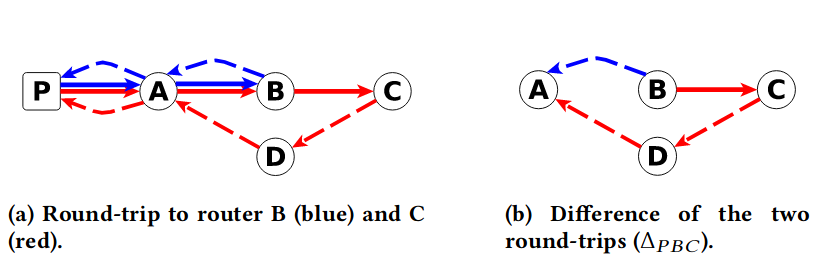
\includegraphics[width=0.7\linewidth]{illustrations/rtt-differ}
	\caption{(a) Le RTT entre la sonde P et les routeurs B et C. (b) La différence entre les  chemins de retour depuis les routeurs B et C vers la sonde P. Source : \cite{DBLP:journals/corr/FontugneAPB16}}
	\label{fig:rtt-differ}
\end{figure} 
Le RTT différentiel $ \Delta_{PBC} $ de la Figure 	\ref{fig:rtt-differ} (b) est décomposé comme suit :
\begin{align}
RTT_{PB} & =  \delta_{PA} + \delta_{AB} + \delta_{BA} + \delta_{AP} \nonumber\\
RTT_{PC} & = \delta_{PA} + \delta_{AB} + \delta_{BC} + \delta_{CD} + \delta_{DA}+ \delta_{AP} \nonumber\\
\Delta_{PBC} & = RTT_{PC} - RTT_{PB}  \label{eq:rttdifference}\\ 
& =  \delta_{BC} + \delta_{CD} + \delta_{DA}- \delta_{BA} \nonumber \\
& = \delta_{BC} + \varepsilon_{PBC} \label{eq:rttdiff}
\end{align}

où $\delta_{BC}$ est le délai du lien $BC$ et $\varepsilon_{PBC}$ est la différence entre les deux chemins de retour : $B$ vers $P$ et $C$ vers $P$.  Le chemin de retour est celui  présenté dans  la Figure \ref{fig:rtt-differ} (b). 
%La première composante dépend de l'état des routeurs $B$ et $C$. La deuxième composante dépend de la sonde $P$. L'analyse du RTT différentiel repose sur la variation de valeurs qu'il prend, au lieu des valeurs exactes, dans  le cas des valeurs exactes, elles peuvent dévier l'interprétation.


\paragraph{Le principe de la détection des changements des délais}~

L'évolution du délai d'un lien est déduit de l'évolution de son RTT différentiel. Reprenons d'abord l'équation (\ref{eq:rttdiff}) du RTT différentiel du lien BC. Les deux variables $\delta_{BC}$ et $\varepsilon_{PBC}$ sont affectées par des facteurs différents.
La valeur de  $\delta_{BC}$ dépend de l'état des deux routeurs B et C et ne dépend pas de la sonde P. Tandis que la valeur de $\varepsilon_{PBC}$ dépend de la sonde P.

Supposons qu'on dispose d'un nombre $n$ de sondes Atlas P$_i$, $i$ $\in$ [$1$, $n$], telles que toutes les sondes ont un chemin de retour  $\varepsilon_{P_{i}BC}$ différent depuis B et depuis C.  Les $n$ RTTs différentiels $\Delta_{P{_i}BC}$ du lien $BC$ pour chacune des sondes $P_i$  partagent la même composante $\delta_{BC}$ :


\begin{align*}
\Delta_{P_{1}BC} &= \delta_{BC} + \varepsilon_{P_{1}BC}\\
\Delta_{P_{2}BC} &= \delta_{BC} + \varepsilon_{P_{2}BC}\\
.... &   ... \\
\Delta_{P_{i}BC} &= \delta_{BC} + \varepsilon_{P_{i}BC}\\
\Delta_{P_{n}BC} &= \delta_{BC} + \varepsilon_{P_{n}BC}\\
\end{align*}

Les valeurs de  $\varepsilon_{P_{i}BC}$ sont  indépendantes. L'indépendance de ces valeurs implique que la distribution $\Delta_{P_{i}BC}$ est estimé  stable au cours du temps si $\delta_{BC}$ est constant. Toutefois, un changement significatif de la valeur de $\delta_{BC}$ influence les valeurs des RTTs différentiels, ainsi,  la distribution des RTTs différentiels $\Delta_{P_{i}BC}$ change. D'où l'idée de l'évolution du délai d'un lien déduit  à partir de l'évolution de son RTT différentiel.

\paragraph{Caractérisation des délais d'un lien}~

Les auteurs du travail de référence \cite{DBLP:journals/corr/FontugneAPB16} ont évalué le délai d'un lien en évaluant son RTT différentiel. Cette évaluation repose sur le théorème central limite énoncé ci-dessous\footnote{Voir le théorème  $ 4.11.1 $ dans \cite{lefebvre2003cours}.}.

\begin{tcolorbox}
	Soient $X_1$, ..., $X_n$ $n$ variables aléatoires \textit{i.i.d}. de moyenne $\mu$ et variance $\sigma^2$ finies ($\sigma > 0$). Soient $S_n$ la somme des $n$ variables aléatoires et 
	\begin{equation}
	Z_n := \frac{S_n - n\mu}{\sqrt{n} \sigma}.
	\end{equation} 
	Alors la fonction de répartition de $Z_n$ tend vers celle d'une loi $N(0,1)$ lorsque $n$ tend vers l'infini.
	
	Remarque : on peut aussi écrire le résultat suivant :
	\begin{equation}
	Sn \approx N(n\mu, n\sigma^2)
	\end{equation}
\end{tcolorbox}

L'application de ce théorème, dans  l'analyse des délais des liens, implique que quelque soit la distribution des RTTs différentiels, la moyenne arithmétique d'un échantillon  est distribuée normalement si la taille de l'échantillon est relativement grande. En pratique,
si un lien subit un changement anormal, la distribution de la moyenne des RTTs différentiels dévie de la distribution normale, par conséquent, la moyenne des RTTs différentiels ayant produit ce changement est identifiée comme  étant une anomalie.

Après avoir évalué les premiers résultats d'application de ce théorème, les auteurs ont conclu que l'utilisation de la médiane,  au lieu de la moyenne, a montré plus de performance en terme de détection des anomalies.
Afin de tenir compte de l'incertitude dans la médiane calculée, ayant la capacité d'identifier un changement anormal, les auteurs ont  calculé  l'intervalle de confiance de cette dernière.
%La distribution des médianes des RTTs différentiels caractérisant un lien est mise à jour tout au long de l'analyse des différentes périodes. 
Par définition\footnote{Definition 2.1 dans \cite{leboudec2010performance}.},  un intervalle de confiance à un niveau $\gamma$,  d'un paramètre $m$ fixé mais inconnu est l'intervalle  $(u(X_1,...,X_n),v(X_1,...,X_n)) $ tel que  :

\begin{align}
\mathbb{P}(u(X_1,...,X_n)< m< v(X_1,...,X_n)) \geq \gamma
\end{align}

\section{L'étude des délais des liens en pratique : l'évolution du RTT différentiel des liens}

L'évolution des RTTs différentiels est une  application du principe décrit dans la section  \ref{principe-de-detection}. Pour un lien donné, le suivi s'étale sur plusieurs  périodes consécutives.  

\subsection{Les étapes principales de détection} \label{steps:detection}
Les étapes du processus de détection peuvent être résumées dans les éléments suivants:

\begin{enumerate}[label=(\roman*)]
	
	\item Vérification de la validité de tout traceroute.
	
	\item Calcul des RTTs différentiels de chaque lien identifié dans les traceroutes.
	
	\item Caractérisation des liens avec le théorème central limite (CLT).
	
	\item  Comparaison de l'état de chaque lien avec sa référence  et l'identification des anomalies.
	
	\item Mise à jour de la référence du lien.
\end{enumerate}

\subsection{Description des paramètres de l'analyse des délais} \label{par:parametre-de-lanalyse}~
La détection des changements des délais nécessite l'ajustement de quelques paramètres. Ces paramètres ont des valeurs par défaut  définies dans le travail de référence. Nous décrivons ci-dessous tous les paramètres : ceux ayant une valeur par défaut et ceux à ajuster :

\begin{description}
	\item[traceroutes] : ce sont l'ensemble des résultats de requêtes traceroute. La détection des anomalies est effectuée suivant le nombre de traceroutes analysés et la période précisée. 
	%Les  traceroutes sont obtenus en utilisant l'API fournie par Atlas.
	\item[start] : c'est la date de début de l'analyse. Seuls les traceroutes effectués par les sondes  à partir de cette date sont analysés.
	\item[end]  : c'est la date marquant la fin de l'analyse. Comme le paramètre \textit{start}, c'est la date maximales des  traceroutes à considérer effectués par les sondes.
	\item[timeWindow]:  ce paramètre est exprimé en secondes. Il correspond à la durée de chaque période des $n$ périodes de l'analyse. Ces périodes ont la même durée. Autrement dit, la durée entre   \textit{start} et \textit{end} est divisée par \textit{timeWindow}. Ceci est illustré à la Figure  \ref{fig:timing_tex_}. Avec $d_i$ dénote le début de la i\up{ème} période,  $i \in [1,n]$. Par défaut, \textit{timeWindow} vaut $ 3600 $ secondes. 
	%illustre le contexte des trois paramètres \textit{start}, \textit{end} et \textit{timeWindow} avec les étapes principales
	\begin{figure}[h]
		\centering
		\captionsetup{justification=centering}
		% Graphic for TeX using PGF
% Title: /home/hayat/RipeAtlasTraceroutesAnalysis/report/illustrations/timing.dia
% Creator: Dia v0.97+git
% CreationDate: Mon Dec  3 23:19:01 2018
% For: hayat
% \usepackage{tikz}
% The following commands are not supported in PSTricks at present
% We define them conditionally, so when they are implemented,
% this pgf file will use them.
\ifx\du\undefined
  \newlength{\du}
\fi
\setlength{\du}{15\unitlength}
\begin{tikzpicture}[even odd rule]
\pgftransformxscale{1.000000}
\pgftransformyscale{-1.000000}
\definecolor{dialinecolor}{rgb}{0.000000, 0.000000, 0.000000}
\pgfsetstrokecolor{dialinecolor}
\pgfsetstrokeopacity{1.000000}
\definecolor{diafillcolor}{rgb}{1.000000, 1.000000, 1.000000}
\pgfsetfillcolor{diafillcolor}
\pgfsetfillopacity{1.000000}
\pgfsetlinewidth{0.100000\du}
\pgfsetdash{}{0pt}
\pgfsetbuttcap
{
\definecolor{diafillcolor}{rgb}{0.000000, 0.000000, 0.000000}
\pgfsetfillcolor{diafillcolor}
\pgfsetfillopacity{1.000000}
% was here!!!
}
\definecolor{dialinecolor}{rgb}{0.000000, 0.000000, 0.000000}
\pgfsetstrokecolor{dialinecolor}
\pgfsetstrokeopacity{1.000000}
\draw (34.600000\du,6.050000\du)--(40.550000\du,6.000000\du);
\pgfsetlinewidth{0.100000\du}
\pgfsetdash{}{0pt}
\pgfsetmiterjoin
\pgfsetbuttcap
\definecolor{dialinecolor}{rgb}{0.000000, 0.000000, 0.000000}
\pgfsetstrokecolor{dialinecolor}
\pgfsetstrokeopacity{1.000000}
\draw (35.097882\du,5.795807\du)--(35.102083\du,6.295790\du);
\pgfsetlinewidth{0.100000\du}
\pgfsetdash{}{0pt}
\pgfsetmiterjoin
\pgfsetbuttcap
\definecolor{dialinecolor}{rgb}{0.000000, 0.000000, 0.000000}
\pgfsetstrokecolor{dialinecolor}
\pgfsetstrokeopacity{1.000000}
\draw (40.052118\du,6.254193\du)--(40.047917\du,5.754210\du);
% setfont left to latex
\definecolor{dialinecolor}{rgb}{0.000000, 0.000000, 0.000000}
\pgfsetstrokecolor{dialinecolor}
\pgfsetstrokeopacity{1.000000}
\definecolor{diafillcolor}{rgb}{0.000000, 0.000000, 0.000000}
\pgfsetfillcolor{diafillcolor}
\pgfsetfillopacity{1.000000}
\node[anchor=base west,inner sep=0pt,outer sep=0pt,color=dialinecolor] at (14.800200\du,8.464650\du){start};
% setfont left to latex
\definecolor{dialinecolor}{rgb}{0.000000, 0.000000, 0.000000}
\pgfsetstrokecolor{dialinecolor}
\pgfsetstrokeopacity{1.000000}
\definecolor{diafillcolor}{rgb}{0.000000, 0.000000, 0.000000}
\pgfsetfillcolor{diafillcolor}
\pgfsetfillopacity{1.000000}
\node[anchor=base west,inner sep=0pt,outer sep=0pt,color=dialinecolor] at (39.375600\du,7.990890\du){end};
% setfont left to latex
\definecolor{dialinecolor}{rgb}{0.000000, 0.000000, 0.000000}
\pgfsetstrokecolor{dialinecolor}
\pgfsetstrokeopacity{1.000000}
\definecolor{diafillcolor}{rgb}{0.000000, 0.000000, 0.000000}
\pgfsetfillcolor{diafillcolor}
\pgfsetfillopacity{1.000000}
\node[anchor=base west,inner sep=0pt,outer sep=0pt,color=dialinecolor] at (24.374800\du,8.977310\du){Périodes de l'analyse};
% setfont left to latex
\definecolor{dialinecolor}{rgb}{0.000000, 0.000000, 0.000000}
\pgfsetstrokecolor{dialinecolor}
\pgfsetstrokeopacity{1.000000}
\definecolor{diafillcolor}{rgb}{0.000000, 0.000000, 0.000000}
\pgfsetfillcolor{diafillcolor}
\pgfsetfillopacity{1.000000}
\node[anchor=base west,inner sep=0pt,outer sep=0pt,color=dialinecolor] at (14.950000\du,7.200000\du){d1};
\pgfsetlinewidth{0.100000\du}
\pgfsetdash{}{0pt}
\pgfsetbuttcap
{
\definecolor{diafillcolor}{rgb}{0.000000, 0.000000, 0.000000}
\pgfsetfillcolor{diafillcolor}
\pgfsetfillopacity{1.000000}
% was here!!!
}
\definecolor{dialinecolor}{rgb}{0.000000, 0.000000, 0.000000}
\pgfsetstrokecolor{dialinecolor}
\pgfsetstrokeopacity{1.000000}
\draw (29.656800\du,6.066270\du)--(35.606800\du,6.016270\du);
\pgfsetlinewidth{0.100000\du}
\pgfsetdash{}{0pt}
\pgfsetmiterjoin
\pgfsetbuttcap
\definecolor{dialinecolor}{rgb}{0.000000, 0.000000, 0.000000}
\pgfsetstrokecolor{dialinecolor}
\pgfsetstrokeopacity{1.000000}
\draw (30.154682\du,5.812077\du)--(30.158883\du,6.312060\du);
\pgfsetlinewidth{0.100000\du}
\pgfsetdash{}{0pt}
\pgfsetmiterjoin
\pgfsetbuttcap
\definecolor{dialinecolor}{rgb}{0.000000, 0.000000, 0.000000}
\pgfsetstrokecolor{dialinecolor}
\pgfsetstrokeopacity{1.000000}
\draw (35.108918\du,6.270463\du)--(35.104717\du,5.770480\du);
\pgfsetlinewidth{0.100000\du}
\pgfsetdash{}{0pt}
\pgfsetbuttcap
{
\definecolor{diafillcolor}{rgb}{0.000000, 0.000000, 0.000000}
\pgfsetfillcolor{diafillcolor}
\pgfsetfillopacity{1.000000}
% was here!!!
}
\definecolor{dialinecolor}{rgb}{0.000000, 0.000000, 0.000000}
\pgfsetstrokecolor{dialinecolor}
\pgfsetstrokeopacity{1.000000}
\draw (24.701800\du,6.106100\du)--(30.651800\du,6.056100\du);
\pgfsetlinewidth{0.100000\du}
\pgfsetdash{}{0pt}
\pgfsetmiterjoin
\pgfsetbuttcap
\definecolor{dialinecolor}{rgb}{0.000000, 0.000000, 0.000000}
\pgfsetstrokecolor{dialinecolor}
\pgfsetstrokeopacity{1.000000}
\draw (25.199682\du,5.851907\du)--(25.203883\du,6.351890\du);
\pgfsetlinewidth{0.100000\du}
\pgfsetdash{}{0pt}
\pgfsetmiterjoin
\pgfsetbuttcap
\definecolor{dialinecolor}{rgb}{0.000000, 0.000000, 0.000000}
\pgfsetstrokecolor{dialinecolor}
\pgfsetstrokeopacity{1.000000}
\draw (30.153918\du,6.310293\du)--(30.149717\du,5.810310\du);
\pgfsetlinewidth{0.100000\du}
\pgfsetdash{}{0pt}
\pgfsetbuttcap
{
\definecolor{diafillcolor}{rgb}{0.000000, 0.000000, 0.000000}
\pgfsetfillcolor{diafillcolor}
\pgfsetfillopacity{1.000000}
% was here!!!
}
\definecolor{dialinecolor}{rgb}{0.000000, 0.000000, 0.000000}
\pgfsetstrokecolor{dialinecolor}
\pgfsetstrokeopacity{1.000000}
\draw (19.796600\du,6.121020\du)--(25.746600\du,6.071020\du);
\pgfsetlinewidth{0.100000\du}
\pgfsetdash{}{0pt}
\pgfsetmiterjoin
\pgfsetbuttcap
\definecolor{dialinecolor}{rgb}{0.000000, 0.000000, 0.000000}
\pgfsetstrokecolor{dialinecolor}
\pgfsetstrokeopacity{1.000000}
\draw (20.294482\du,5.866827\du)--(20.298683\du,6.366810\du);
\pgfsetlinewidth{0.100000\du}
\pgfsetdash{}{0pt}
\pgfsetmiterjoin
\pgfsetbuttcap
\definecolor{dialinecolor}{rgb}{0.000000, 0.000000, 0.000000}
\pgfsetstrokecolor{dialinecolor}
\pgfsetstrokeopacity{1.000000}
\draw (25.248718\du,6.325213\du)--(25.244517\du,5.825230\du);
\pgfsetlinewidth{0.100000\du}
\pgfsetdash{}{0pt}
\pgfsetbuttcap
{
\definecolor{diafillcolor}{rgb}{0.000000, 0.000000, 0.000000}
\pgfsetfillcolor{diafillcolor}
\pgfsetfillopacity{1.000000}
% was here!!!
}
\definecolor{dialinecolor}{rgb}{0.000000, 0.000000, 0.000000}
\pgfsetstrokecolor{dialinecolor}
\pgfsetstrokeopacity{1.000000}
\draw (14.841600\du,6.135940\du)--(20.791600\du,6.085940\du);
\pgfsetlinewidth{0.100000\du}
\pgfsetdash{}{0pt}
\pgfsetmiterjoin
\pgfsetbuttcap
\definecolor{dialinecolor}{rgb}{0.000000, 0.000000, 0.000000}
\pgfsetstrokecolor{dialinecolor}
\pgfsetstrokeopacity{1.000000}
\draw (15.339482\du,5.881747\du)--(15.343683\du,6.381730\du);
\pgfsetlinewidth{0.100000\du}
\pgfsetdash{}{0pt}
\pgfsetmiterjoin
\pgfsetbuttcap
\definecolor{dialinecolor}{rgb}{0.000000, 0.000000, 0.000000}
\pgfsetstrokecolor{dialinecolor}
\pgfsetstrokeopacity{1.000000}
\draw (20.293718\du,6.340133\du)--(20.289517\du,5.840150\du);
% setfont left to latex
\definecolor{dialinecolor}{rgb}{0.000000, 0.000000, 0.000000}
\pgfsetstrokecolor{dialinecolor}
\pgfsetstrokeopacity{1.000000}
\definecolor{diafillcolor}{rgb}{0.000000, 0.000000, 0.000000}
\pgfsetfillcolor{diafillcolor}
\pgfsetfillopacity{1.000000}
\node[anchor=base west,inner sep=0pt,outer sep=0pt,color=dialinecolor] at (19.845000\du,7.235000\du){d2};
% setfont left to latex
\definecolor{dialinecolor}{rgb}{0.000000, 0.000000, 0.000000}
\pgfsetstrokecolor{dialinecolor}
\pgfsetstrokeopacity{1.000000}
\definecolor{diafillcolor}{rgb}{0.000000, 0.000000, 0.000000}
\pgfsetfillcolor{diafillcolor}
\pgfsetfillopacity{1.000000}
\node[anchor=base west,inner sep=0pt,outer sep=0pt,color=dialinecolor] at (24.750000\du,7.300000\du){d3};
% setfont left to latex
\definecolor{dialinecolor}{rgb}{0.000000, 0.000000, 0.000000}
\pgfsetstrokecolor{dialinecolor}
\pgfsetstrokeopacity{1.000000}
\definecolor{diafillcolor}{rgb}{0.000000, 0.000000, 0.000000}
\pgfsetfillcolor{diafillcolor}
\pgfsetfillopacity{1.000000}
\node[anchor=base west,inner sep=0pt,outer sep=0pt,color=dialinecolor] at (29.740000\du,7.175000\du){di};
% setfont left to latex
\definecolor{dialinecolor}{rgb}{0.000000, 0.000000, 0.000000}
\pgfsetstrokecolor{dialinecolor}
\pgfsetstrokeopacity{1.000000}
\definecolor{diafillcolor}{rgb}{0.000000, 0.000000, 0.000000}
\pgfsetfillcolor{diafillcolor}
\pgfsetfillopacity{1.000000}
\node[anchor=base west,inner sep=0pt,outer sep=0pt,color=dialinecolor] at (34.685000\du,7.165000\du){di+1};
\pgfsetlinewidth{0.100000\du}
\pgfsetdash{}{0pt}
\pgfsetbuttcap
\definecolor{dialinecolor}{rgb}{0.000000, 0.000000, 0.000000}
\pgfsetstrokecolor{dialinecolor}
\pgfsetstrokeopacity{1.000000}
\pgfpathmoveto{\pgfpoint{25.180033\du}{4.900033\du}}
\pgfpatharc{315}{226}{3.501250\du and 3.501250\du}
\pgfusepath{stroke}
% setfont left to latex
\definecolor{dialinecolor}{rgb}{0.000000, 0.000000, 0.000000}
\pgfsetstrokecolor{dialinecolor}
\pgfsetstrokeopacity{1.000000}
\definecolor{diafillcolor}{rgb}{0.000000, 0.000000, 0.000000}
\pgfsetfillcolor{diafillcolor}
\pgfsetfillopacity{1.000000}
\node[anchor=base west,inner sep=0pt,outer sep=0pt,color=dialinecolor] at (20.780000\du,3.400000\du){timeWindow};
\pgfsetlinewidth{0.100000\du}
\pgfsetdash{}{0pt}
\pgfsetbuttcap
\definecolor{dialinecolor}{rgb}{0.000000, 0.000000, 0.000000}
\pgfsetstrokecolor{dialinecolor}
\pgfsetstrokeopacity{1.000000}
\pgfpathmoveto{\pgfpoint{29.975033\du}{4.885033\du}}
\pgfpatharc{315}{226}{3.501250\du and 3.501250\du}
\pgfusepath{stroke}
% setfont left to latex
\definecolor{dialinecolor}{rgb}{0.000000, 0.000000, 0.000000}
\pgfsetstrokecolor{dialinecolor}
\pgfsetstrokeopacity{1.000000}
\definecolor{diafillcolor}{rgb}{0.000000, 0.000000, 0.000000}
\pgfsetfillcolor{diafillcolor}
\pgfsetfillopacity{1.000000}
\node[anchor=base west,inner sep=0pt,outer sep=0pt,color=dialinecolor] at (25.675000\du,3.485000\du){timeWindow};
\pgfsetlinewidth{0.100000\du}
\pgfsetdash{}{0pt}
\pgfsetbuttcap
\definecolor{dialinecolor}{rgb}{0.000000, 0.000000, 0.000000}
\pgfsetstrokecolor{dialinecolor}
\pgfsetstrokeopacity{1.000000}
\pgfpathmoveto{\pgfpoint{20.275033\du}{4.785033\du}}
\pgfpatharc{315}{226}{3.501250\du and 3.501250\du}
\pgfusepath{stroke}
% setfont left to latex
\definecolor{dialinecolor}{rgb}{0.000000, 0.000000, 0.000000}
\pgfsetstrokecolor{dialinecolor}
\pgfsetstrokeopacity{1.000000}
\definecolor{diafillcolor}{rgb}{0.000000, 0.000000, 0.000000}
\pgfsetfillcolor{diafillcolor}
\pgfsetfillopacity{1.000000}
\node[anchor=base west,inner sep=0pt,outer sep=0pt,color=dialinecolor] at (16.025000\du,3.435000\du){timeWindow};
\end{tikzpicture}

		\caption{Illustration des périodes de l'analyse entre la date de début et la date de fin.}
		\label{fig:timing_tex_}
	\end{figure}
	%\begin{figure}[h]	
	%	\centering
	%	\resizebox{\textwidth}{!}{
	%		% Graphic for TeX using PGF
% Title: /home/bellafkih/Documents/2018-2019/memoire/rapport_memoire/dia/timewindow.dia
% Creator: Dia v0.97.3
% CreationDate: Sun Oct  7 15:34:20 2018
% For: bellafkih
% \usepackage{tikz}
% The following commands are not supported in PSTricks at present
% We define them conditionally, so when they are implemented,
% this pgf file will use them.
\ifx\du\undefined
  \newlength{\du}
\fi
\setlength{\du}{15\unitlength}
\begin{tikzpicture}
\pgftransformxscale{1.000000}
\pgftransformyscale{-1.000000}
\definecolor{dialinecolor}{rgb}{0.000000, 0.000000, 0.000000}
\pgfsetstrokecolor{dialinecolor}
\definecolor{dialinecolor}{rgb}{1.000000, 1.000000, 1.000000}
\pgfsetfillcolor{dialinecolor}
\pgfsetlinewidth{0.200000\du}
\pgfsetdash{}{0pt}
\pgfsetdash{}{0pt}
\pgfsetbuttcap
{
\definecolor{dialinecolor}{rgb}{0.000000, 0.000000, 0.000000}
\pgfsetfillcolor{dialinecolor}
% was here!!!
\pgfsetarrowsend{to}
\definecolor{dialinecolor}{rgb}{0.000000, 0.000000, 0.000000}
\pgfsetstrokecolor{dialinecolor}
\draw (10.000000\du,2.000000\du)--(10.000000\du,26.650000\du);
}
% setfont left to latex
\definecolor{dialinecolor}{rgb}{0.000000, 0.000000, 0.000000}
\pgfsetstrokecolor{dialinecolor}
\node[anchor=west] at (7.650000\du,2.050000\du){start};
% setfont left to latex
\definecolor{dialinecolor}{rgb}{0.000000, 0.000000, 0.000000}
\pgfsetstrokecolor{dialinecolor}
\node[anchor=west] at (7.850000\du,22.100000\du){end};
\pgfsetlinewidth{0.000000\du}
\pgfsetdash{}{0pt}
\pgfsetdash{}{0pt}
\pgfsetbuttcap
{
\definecolor{dialinecolor}{rgb}{0.000000, 0.000000, 0.000000}
\pgfsetfillcolor{dialinecolor}
% was here!!!
\definecolor{dialinecolor}{rgb}{0.000000, 0.000000, 0.000000}
\pgfsetstrokecolor{dialinecolor}
\draw (10.600000\du,2.000000\du)--(9.450000\du,2.000000\du);
}
\pgfsetlinewidth{0.000000\du}
\pgfsetdash{}{0pt}
\pgfsetdash{}{0pt}
\pgfsetbuttcap
{
\definecolor{dialinecolor}{rgb}{0.000000, 0.000000, 0.000000}
\pgfsetfillcolor{dialinecolor}
% was here!!!
\definecolor{dialinecolor}{rgb}{0.000000, 0.000000, 0.000000}
\pgfsetstrokecolor{dialinecolor}
\draw (10.585000\du,5.960000\du)--(9.435000\du,5.960000\du);
}
\pgfsetlinewidth{0.000000\du}
\pgfsetdash{}{0pt}
\pgfsetdash{}{0pt}
\pgfsetbuttcap
{
\definecolor{dialinecolor}{rgb}{0.000000, 0.000000, 0.000000}
\pgfsetfillcolor{dialinecolor}
% was here!!!
\definecolor{dialinecolor}{rgb}{0.000000, 0.000000, 0.000000}
\pgfsetstrokecolor{dialinecolor}
\draw (10.570000\du,10.020000\du)--(9.420000\du,10.020000\du);
}
\pgfsetlinewidth{0.000000\du}
\pgfsetdash{}{0pt}
\pgfsetdash{}{0pt}
\pgfsetbuttcap
{
\definecolor{dialinecolor}{rgb}{0.000000, 0.000000, 0.000000}
\pgfsetfillcolor{dialinecolor}
% was here!!!
\definecolor{dialinecolor}{rgb}{0.000000, 0.000000, 0.000000}
\pgfsetstrokecolor{dialinecolor}
\draw (10.505000\du,13.930000\du)--(9.355000\du,13.930000\du);
}
\pgfsetlinewidth{0.000000\du}
\pgfsetdash{}{0pt}
\pgfsetdash{}{0pt}
\pgfsetbuttcap
{
\definecolor{dialinecolor}{rgb}{0.000000, 0.000000, 0.000000}
\pgfsetfillcolor{dialinecolor}
% was here!!!
\definecolor{dialinecolor}{rgb}{0.000000, 0.000000, 0.000000}
\pgfsetstrokecolor{dialinecolor}
\draw (10.540000\du,17.940000\du)--(9.390000\du,17.940000\du);
}
\pgfsetlinewidth{0.000000\du}
\pgfsetdash{}{0pt}
\pgfsetdash{}{0pt}
\pgfsetbuttcap
{
\definecolor{dialinecolor}{rgb}{0.000000, 0.000000, 0.000000}
\pgfsetfillcolor{dialinecolor}
% was here!!!
\definecolor{dialinecolor}{rgb}{0.000000, 0.000000, 0.000000}
\pgfsetstrokecolor{dialinecolor}
\draw (10.575000\du,22.050000\du)--(9.425000\du,22.050000\du);
}
\pgfsetlinewidth{0.000000\du}
\pgfsetdash{}{0pt}
\pgfsetdash{}{0pt}
\pgfsetbuttcap
{
\definecolor{dialinecolor}{rgb}{0.000000, 0.000000, 0.000000}
\pgfsetfillcolor{dialinecolor}
% was here!!!
\pgfsetarrowsstart{to}
\pgfsetarrowsend{to}
\definecolor{dialinecolor}{rgb}{0.000000, 0.000000, 0.000000}
\pgfsetstrokecolor{dialinecolor}
\pgfpathmoveto{\pgfpoint{6.950071\du}{2.049940\du}}
\pgfpatharc{231}{129}{2.448949\du and 2.448949\du}
\pgfusepath{stroke}
}
% setfont left to latex
\definecolor{dialinecolor}{rgb}{0.000000, 0.000000, 0.000000}
\pgfsetstrokecolor{dialinecolor}
\node[anchor=west] at (2.150000\du,26.900000\du){Temps en secondes (s)};
\pgfsetlinewidth{0.000000\du}
\pgfsetdash{}{0pt}
\pgfsetdash{}{0pt}
\pgfsetbuttcap
{
\definecolor{dialinecolor}{rgb}{0.000000, 0.000000, 0.000000}
\pgfsetfillcolor{dialinecolor}
% was here!!!
\pgfsetarrowsstart{to}
\pgfsetarrowsend{to}
\definecolor{dialinecolor}{rgb}{0.000000, 0.000000, 0.000000}
\pgfsetstrokecolor{dialinecolor}
\pgfpathmoveto{\pgfpoint{7.049251\du}{6.119940\du}}
\pgfpatharc{231}{129}{2.448949\du and 2.448949\du}
\pgfusepath{stroke}
}
\pgfsetlinewidth{0.000000\du}
\pgfsetdash{}{0pt}
\pgfsetdash{}{0pt}
\pgfsetbuttcap
{
\definecolor{dialinecolor}{rgb}{0.000000, 0.000000, 0.000000}
\pgfsetfillcolor{dialinecolor}
% was here!!!
\pgfsetarrowsstart{to}
\pgfsetarrowsend{to}
\definecolor{dialinecolor}{rgb}{0.000000, 0.000000, 0.000000}
\pgfsetstrokecolor{dialinecolor}
\pgfpathmoveto{\pgfpoint{6.984251\du}{10.079940\du}}
\pgfpatharc{231}{129}{2.448949\du and 2.448949\du}
\pgfusepath{stroke}
}
\pgfsetlinewidth{0.000000\du}
\pgfsetdash{}{0pt}
\pgfsetdash{}{0pt}
\pgfsetbuttcap
{
\definecolor{dialinecolor}{rgb}{0.000000, 0.000000, 0.000000}
\pgfsetfillcolor{dialinecolor}
% was here!!!
\pgfsetarrowsstart{to}
\pgfsetarrowsend{to}
\definecolor{dialinecolor}{rgb}{0.000000, 0.000000, 0.000000}
\pgfsetstrokecolor{dialinecolor}
\pgfpathmoveto{\pgfpoint{6.869251\du}{14.089940\du}}
\pgfpatharc{231}{129}{2.448949\du and 2.448949\du}
\pgfusepath{stroke}
}
\pgfsetlinewidth{0.000000\du}
\pgfsetdash{}{0pt}
\pgfsetdash{}{0pt}
\pgfsetbuttcap
{
\definecolor{dialinecolor}{rgb}{0.000000, 0.000000, 0.000000}
\pgfsetfillcolor{dialinecolor}
% was here!!!
\pgfsetarrowsstart{to}
\pgfsetarrowsend{to}
\definecolor{dialinecolor}{rgb}{0.000000, 0.000000, 0.000000}
\pgfsetstrokecolor{dialinecolor}
\pgfpathmoveto{\pgfpoint{6.954251\du}{18.099940\du}}
\pgfpatharc{231}{129}{2.448949\du and 2.448949\du}
\pgfusepath{stroke}
}
% setfont left to latex
\definecolor{dialinecolor}{rgb}{0.000000, 0.000000, 0.000000}
\pgfsetstrokecolor{dialinecolor}
\node[anchor=west] at (0.650000\du,4.050000\du){timeWindow s};
% setfont left to latex
\definecolor{dialinecolor}{rgb}{0.000000, 0.000000, 0.000000}
\pgfsetstrokecolor{dialinecolor}
\node[anchor=west] at (0.685100\du,8.005000\du){timeWindow s};
% setfont left to latex
\definecolor{dialinecolor}{rgb}{0.000000, 0.000000, 0.000000}
\pgfsetstrokecolor{dialinecolor}
\node[anchor=west] at (0.870100\du,12.015000\du){timeWindow s};
% setfont left to latex
\definecolor{dialinecolor}{rgb}{0.000000, 0.000000, 0.000000}
\pgfsetstrokecolor{dialinecolor}
\node[anchor=west] at (0.905100\du,16.025000\du){timeWindow s};
% setfont left to latex
\definecolor{dialinecolor}{rgb}{0.000000, 0.000000, 0.000000}
\pgfsetstrokecolor{dialinecolor}
\node[anchor=west] at (1.040100\du,19.935000\du){timeWindow s};
% setfont left to latex
\definecolor{dialinecolor}{rgb}{0.000000, 0.000000, 0.000000}
\pgfsetstrokecolor{dialinecolor}
\node[anchor=west] at (11.200100\du,3.850000\du){appliquer : computeRtt(), mergeRttResults(), outlierDetection()};
% setfont left to latex
\definecolor{dialinecolor}{rgb}{0.000000, 0.000000, 0.000000}
\pgfsetstrokecolor{dialinecolor}
\node[anchor=west] at (11.035100\du,7.905000\du){appliquer : computeRtt(), mergeRttResults(), outlierDetection()};
% setfont left to latex
\definecolor{dialinecolor}{rgb}{0.000000, 0.000000, 0.000000}
\pgfsetstrokecolor{dialinecolor}
\node[anchor=west] at (11.120100\du,12.015000\du){appliquer : computeRtt(), mergeRttResults(), outlierDetection()};
% setfont left to latex
\definecolor{dialinecolor}{rgb}{0.000000, 0.000000, 0.000000}
\pgfsetstrokecolor{dialinecolor}
\node[anchor=west] at (11.105100\du,15.875000\du){appliquer : computeRtt(), mergeRttResults(), outlierDetection()};
% setfont left to latex
\definecolor{dialinecolor}{rgb}{0.000000, 0.000000, 0.000000}
\pgfsetstrokecolor{dialinecolor}
\node[anchor=west] at (11.040100\du,19.885000\du){appliquer : computeRtt(), mergeRttResults(), outlierDetection()};
% setfont left to latex
\definecolor{dialinecolor}{rgb}{0.000000, 0.000000, 0.000000}
\pgfsetstrokecolor{dialinecolor}
\node[anchor=west] at (11.950100\du,2.000000\du){inputs : paramère de l'expérience};
% setfont left to latex
\definecolor{dialinecolor}{rgb}{0.000000, 0.000000, 0.000000}
\pgfsetstrokecolor{dialinecolor}
\node[anchor=west] at (12.050100\du,22.000000\du){output : les changements détéctés et ses caractériqtiques};
\end{tikzpicture}
 
	%	}
	%	\caption{Illustration du paramètre timeWindow}
	%	\label{fig:timewindow}
	%\end{figure}
	\item[minSeen] : est le nombre de fenêtres à atteindre avant de commencer la comparaison du RTT différentiel d'un lien avec sa référence. 
	%comme l'analyse des liens est réalisée sur plusieurs périodes de durée \textit{timeWindow}, 
	%ce paramètre est un entier, il indique le déclenchement de la comparaison du RTT différentiel de référence d'un lien avec sa valeur courante.  
	%Par exemple, si $ minSeen = 24 $ et $timeWindow = 3600$ (1 heure), cela implique que la première référence de tout lien est construite des valeurs obtenues tout au long la durée $24 * timeWindow$, donc après avoir analysé les traceroutes d'une journée. A la 25\up{ème} \textit{timeWindow}, la détection des anomalies s'effectue.
	% nombre de fois à partir desquelles on peut  vérifier son RTT différentiel; s'il indique une anomalie ou non. 
	%Par exemple, un lien peut être identifié dans $3$ $d_i$, ou bien être identifié  une seule fois durant toute la période de l'analyse.
	
	\item[alpha ]: noté $\alpha$,  $\alpha \in [0, 1]$, c'est le paramètre de la  moyenne mobile exponentielle calculée.
	%\guillemotleft \textit{ Les méthodes de lissage exponentiel  sont un ensemble de techniques empiriques de prévision qui accordent plus ou moins d'importance aux valeurs du passé d'une série temporelle\footnote{Source : \url{https://perso.math.univ-toulouse.fr/lagnoux/files/2013/12/Chap6.pdf}, consultée le $30/09/2018.$}}. \guillemotright
	
	La  moyenne mobile exponentielle est utilisée pour calculer la moyenne des RTTs différentiels de référence durant une période $d_k$.
	% Cette médiane constitue une référence  sur laquelle se base la détection des anomalies.
	La  valeur de la médiane des RTTs différentiels de référence $ \overline{m}_{t}$   pour la période $ t $ et  le lien $l$ :
	\begin{align*}
	\overline{m}_{t} &=  \alpha{m}_{t} + (1 -  \alpha)  \overline{m}_{t-1}
	\end{align*} 
	$m_t$ la médiane des RTTs différentiels observée pour $l$ durant la \textit{période} $t$. 
	
	$ \overline{m}_{t-1}$  la médiane des  RTTs différentiels  de référence durant la \textit{période} $ t-1 $.  
	
	
	
	Pour précision, \{$m_t$\} et \{$ \overline{m}_{t}$\} désignent deux ensembles différents.   Le premier est l'ensemble des médianes des RTTs différentiels de chaque période $d_k$. Or, le deuxième est l'ensemble des médianes des RTTs différentiels, de référence, construite en utilisant la méthode de la moyenne mobile exponentielle. Le calcul de cette dernière prend en compte les médianes des RTTs différentiels précédentes ainsi que la médiane des RTTs différentiels courante. La participation de ces dernières dans le calcul de la référence est dirigé par le paramètre $\alpha$. Plus de détails sur ce calcul est donné dans la section[!]. 
	%La  valeur de la médiane de référence  $ \overline{m}_{t}$ de la période $t$ est obtenue par: 
	
	
	
	Le paramètre $\alpha$  contrôle l'importance  des mesures précédentes par rapport aux mesures récentes. De ce fait, \guillemotleft \textit{plus $\alpha$ est proche de $ 1 $ plus les observations récentes influent sur la prévision, à l'inverse un $\alpha$ proche de $0$ conduit à une prévision très stable prenant en compte un passé lointain}\footnote{Voir le Lissages Exponentiels dans \url{https://www.math.u-psud.fr/~goude/Materials/time_series/cours3_lissage_expo.pdf}, consultée le $30/09/2018$.}.\guillemotright.  Dans le travail de référence, le paramètre $\alpha$  vaut par défaut $0.01$.
	
	
	\item[confInterval] : ce paramètre indique le niveau de confiance de l'intervalle de confiance de la médiane calculée des RTTs différentiels. Précisément, cet intervalle de confiance calculé est de niveau de confiance égal à $ 1 - confInterval $.  L'intervalle de confiance d'une moyenne  est défini comme représentant les valeurs probables que peut prendre cette moyenne, si on accepte une marge d'erreur définie à l'avance. Il existe plusieurs méthodes pour calculer l'intervalle de confiance d'une proportion. Parmi les critères impliqués sur le choix de la méthode du calcul, on note le nombre total d'expériences.
	
	Au RTT différentiel courant et  au celui de référence d'un lien donné sont associés des intervalles de confiance.  le calcul des intervalles de confiance  est approché par le score de Wilson. Le score de wilson a été adopté car il donne des résultats même si la distribution pour laquelle l'intervalle de confiance est calculé est petite. Pour chaque lien et pour chaque période $d_k$,  deux intervalles de confiances sont calculés, pour ensuite évaluer le chevauchement entre ces deux intervalles. L'outil de détection utilise une marge d'erreur égale à  $ 0.05 $. Les détails du calcul des intervalles de confiances sont fournis dans la section[!].
\end{description}


\subsection{Processus de  détection des anomalies  : notation formelle}\label{steps-rtt-analysis}

Soient $ d_1 $, $  d_2 $, $d_k$, ..., $ d_n $ l'ensemble $D$ de $n$ périodes entre \textit{start} et \textit{end} avec $k \in [1,n]$. La différence entre le début de la période $ d_{k+1} $ et le début de la période $ d_k $ est égale à $timeWindow$ pour tout $k+1 \leq n $.  

Le processus de la détection des anomalies passe par plusieurs étapes. D'abord on  regroupe les traceroutes à analyser par période $d_k$ (étape $ 1 $). Ensuite, on prépare les traceroutes de toute  période $d_k$ en y appliquant un nombre d'opérations (étapes  $ 2 $ à $ 6 $) afin d'énumérer les liens possibles avec leurs RTTs différentiels. A la fin de la préparation des traceroutes de toutes les périodes, nous obtenons une liste de liens par période. Nous résumons ensuite ces liens en fusionnant les mêmes liens identifiés durant toutes les périodes tout en conservant la période pendant laquelle il a été identifié. Sur base des détails d'un lien donné,  nous identifions les anomalies dans leurs délais (étapes $ 7 $ à $9$). 

\subparagraph{Notations}
Chaque traceroute contient un ensemble de sauts, et chaque saut contient un ensemble de signaux. Chaque signal se caractérise par le routeur émettant ce signal et le RTT correspondant. 
Soit  $h_i$ le i\up{ème} saut d'un traceroute donné tel que $h_i =\{s_{i,j} |  j \in [1, S], i\in [1,H]  \}$, $S$ et $H$ sont des entiers. Soit $ s_{i,j} $  le j\up{ème} signal du i\up{ème} saut, il se caractérise par le routeur  source du signal $from_{i,j}$ et le RTT correspondant est $rtt_{i,j}$.

Un traceroute  est un ensemble de sauts $h_i$ dans l'ensemble  $H$ auxquels sont joints l'identifiant de la sonde ayant effectué la requête traceroute et la destination de la requête. Chaque saut est décrit par un ensemble de signaux dans  $S$.  Chaque signal décrit le routeur ayant émis une réponse à la sonde parmi les routeurs traversés avant d'atteindre la destination finale.  Pour le saut $h_i$, on note trois\footnote{Le nombre trois peut varier dans certains cas. L'outil de détection conçu est adapté à tout nombre de signaux.} signaux $s_{i, j},  j\in [1,3]$ dont le routeur émettant le signal est $from_{i,j}$ et son RTT est égal à $rtt_{i,j}$. C'est ce qu'illustre  la Figure \ref{fig:traceroute}.

\begin{figure}[H]
	\centering
	\captionsetup{justification=centering}
	\resizebox{\textwidth}{!}{
		% Graphic for TeX using PGF
% Title: /home/hayat/RipeAtlasTraceroutesAnalysis/report/illustrations/dia/traceroute_.dia
% Creator: Dia v0.97+git
% CreationDate: Fri Dec 28 18:14:49 2018
% For: hayat
% \usepackage{tikz}
% The following commands are not supported in PSTricks at present
% We define them conditionally, so when they are implemented,
% this pgf file will use them.
\ifx\du\undefined
  \newlength{\du}
\fi
\setlength{\du}{15\unitlength}
\begin{tikzpicture}[even odd rule]
\pgftransformxscale{1.000000}
\pgftransformyscale{-1.000000}
\definecolor{dialinecolor}{rgb}{0.000000, 0.000000, 0.000000}
\pgfsetstrokecolor{dialinecolor}
\pgfsetstrokeopacity{1.000000}
\definecolor{diafillcolor}{rgb}{1.000000, 1.000000, 1.000000}
\pgfsetfillcolor{diafillcolor}
\pgfsetfillopacity{1.000000}
\pgfsetlinewidth{0.100000\du}
\pgfsetdash{}{0pt}
\pgfsetmiterjoin
{\pgfsetcornersarced{\pgfpoint{0.000000\du}{0.000000\du}}\definecolor{diafillcolor}{rgb}{1.000000, 1.000000, 1.000000}
\pgfsetfillcolor{diafillcolor}
\pgfsetfillopacity{1.000000}
\fill (2.487500\du,12.100000\du)--(2.487500\du,14.000000\du)--(5.712500\du,14.000000\du)--(5.712500\du,12.100000\du)--cycle;
}{\pgfsetcornersarced{\pgfpoint{0.000000\du}{0.000000\du}}\definecolor{dialinecolor}{rgb}{0.000000, 0.000000, 0.000000}
\pgfsetstrokecolor{dialinecolor}
\pgfsetstrokeopacity{1.000000}
\draw (2.487500\du,12.100000\du)--(2.487500\du,14.000000\du)--(5.712500\du,14.000000\du)--(5.712500\du,12.100000\du)--cycle;
}% setfont left to latex
\definecolor{dialinecolor}{rgb}{0.000000, 0.000000, 0.000000}
\pgfsetstrokecolor{dialinecolor}
\pgfsetstrokeopacity{1.000000}
\definecolor{diafillcolor}{rgb}{0.000000, 0.000000, 0.000000}
\pgfsetfillcolor{diafillcolor}
\pgfsetfillopacity{1.000000}
\node[anchor=base,inner sep=0pt, outer sep=0pt,color=dialinecolor] at (4.100000\du,13.245000\du){source};
\pgfsetlinewidth{0.100000\du}
\pgfsetdash{}{0pt}
\pgfsetmiterjoin
{\pgfsetcornersarced{\pgfpoint{0.000000\du}{0.000000\du}}\definecolor{diafillcolor}{rgb}{1.000000, 1.000000, 1.000000}
\pgfsetfillcolor{diafillcolor}
\pgfsetfillopacity{1.000000}
\fill (46.257500\du,11.850000\du)--(46.257500\du,13.750000\du)--(50.942500\du,13.750000\du)--(50.942500\du,11.850000\du)--cycle;
}{\pgfsetcornersarced{\pgfpoint{0.000000\du}{0.000000\du}}\definecolor{dialinecolor}{rgb}{0.000000, 0.000000, 0.000000}
\pgfsetstrokecolor{dialinecolor}
\pgfsetstrokeopacity{1.000000}
\draw (46.257500\du,11.850000\du)--(46.257500\du,13.750000\du)--(50.942500\du,13.750000\du)--(50.942500\du,11.850000\du)--cycle;
}% setfont left to latex
\definecolor{dialinecolor}{rgb}{0.000000, 0.000000, 0.000000}
\pgfsetstrokecolor{dialinecolor}
\pgfsetstrokeopacity{1.000000}
\definecolor{diafillcolor}{rgb}{0.000000, 0.000000, 0.000000}
\pgfsetfillcolor{diafillcolor}
\pgfsetfillopacity{1.000000}
\node[anchor=base,inner sep=0pt, outer sep=0pt,color=dialinecolor] at (48.600000\du,12.995000\du){destination};
\pgfsetlinewidth{0.100000\du}
\pgfsetdash{}{0pt}
\pgfsetmiterjoin
\definecolor{diafillcolor}{rgb}{1.000000, 1.000000, 1.000000}
\pgfsetfillcolor{diafillcolor}
\pgfsetfillopacity{1.000000}
\pgfpathellipse{\pgfpoint{11.648369\du}{12.925048\du}}{\pgfpoint{1.195569\du}{0\du}}{\pgfpoint{0\du}{1.078448\du}}
\pgfusepath{fill}
\definecolor{dialinecolor}{rgb}{0.000000, 0.000000, 0.000000}
\pgfsetstrokecolor{dialinecolor}
\pgfsetstrokeopacity{1.000000}
\pgfpathellipse{\pgfpoint{11.648369\du}{12.925048\du}}{\pgfpoint{1.195569\du}{0\du}}{\pgfpoint{0\du}{1.078448\du}}
\pgfusepath{stroke}
% setfont left to latex
\definecolor{dialinecolor}{rgb}{0.000000, 0.000000, 0.000000}
\pgfsetstrokecolor{dialinecolor}
\pgfsetstrokeopacity{1.000000}
\definecolor{diafillcolor}{rgb}{0.000000, 0.000000, 0.000000}
\pgfsetfillcolor{diafillcolor}
\pgfsetfillopacity{1.000000}
\node[anchor=base,inner sep=0pt, outer sep=0pt,color=dialinecolor] at (11.648369\du,13.120048\du){R1};
\pgfsetlinewidth{0.100000\du}
\pgfsetdash{}{0pt}
\pgfsetmiterjoin
\definecolor{diafillcolor}{rgb}{1.000000, 1.000000, 1.000000}
\pgfsetfillcolor{diafillcolor}
\pgfsetfillopacity{1.000000}
\pgfpathellipse{\pgfpoint{26.640569\du}{13.018448\du}}{\pgfpoint{1.195569\du}{0\du}}{\pgfpoint{0\du}{1.078448\du}}
\pgfusepath{fill}
\definecolor{dialinecolor}{rgb}{0.000000, 0.000000, 0.000000}
\pgfsetstrokecolor{dialinecolor}
\pgfsetstrokeopacity{1.000000}
\pgfpathellipse{\pgfpoint{26.640569\du}{13.018448\du}}{\pgfpoint{1.195569\du}{0\du}}{\pgfpoint{0\du}{1.078448\du}}
\pgfusepath{stroke}
% setfont left to latex
\definecolor{dialinecolor}{rgb}{0.000000, 0.000000, 0.000000}
\pgfsetstrokecolor{dialinecolor}
\pgfsetstrokeopacity{1.000000}
\definecolor{diafillcolor}{rgb}{0.000000, 0.000000, 0.000000}
\pgfsetfillcolor{diafillcolor}
\pgfsetfillopacity{1.000000}
\node[anchor=base,inner sep=0pt, outer sep=0pt,color=dialinecolor] at (26.640569\du,13.213448\du){R2};
\pgfsetlinewidth{0.100000\du}
\pgfsetdash{}{0pt}
\pgfsetbuttcap
{
\definecolor{diafillcolor}{rgb}{0.000000, 0.000000, 0.000000}
\pgfsetfillcolor{diafillcolor}
\pgfsetfillopacity{1.000000}
% was here!!!
\definecolor{dialinecolor}{rgb}{0.000000, 0.000000, 0.000000}
\pgfsetstrokecolor{dialinecolor}
\pgfsetstrokeopacity{1.000000}
\draw (5.750239\du,13.017555\du)--(10.452800\du,12.925100\du);
}
\pgfsetlinewidth{0.100000\du}
\pgfsetdash{}{0pt}
\pgfsetbuttcap
{
\definecolor{diafillcolor}{rgb}{0.000000, 0.000000, 0.000000}
\pgfsetfillcolor{diafillcolor}
\pgfsetfillopacity{1.000000}
% was here!!!
\definecolor{dialinecolor}{rgb}{0.000000, 0.000000, 0.000000}
\pgfsetstrokecolor{dialinecolor}
\pgfsetstrokeopacity{1.000000}
\draw (12.844000\du,12.925100\du)--(25.445000\du,13.018448\du);
}
\pgfsetlinewidth{0.100000\du}
\pgfsetdash{}{0pt}
\pgfsetbuttcap
{
\definecolor{diafillcolor}{rgb}{0.000000, 0.000000, 0.000000}
\pgfsetfillcolor{diafillcolor}
\pgfsetfillopacity{1.000000}
% was here!!!
\definecolor{dialinecolor}{rgb}{0.000000, 0.000000, 0.000000}
\pgfsetstrokecolor{dialinecolor}
\pgfsetstrokeopacity{1.000000}
\draw (39.886138\du,12.818448\du)--(46.257500\du,12.800000\du);
}
% setfont left to latex
\definecolor{dialinecolor}{rgb}{0.000000, 0.000000, 0.000000}
\pgfsetstrokecolor{dialinecolor}
\pgfsetstrokeopacity{1.000000}
\definecolor{diafillcolor}{rgb}{0.000000, 0.000000, 0.000000}
\pgfsetfillcolor{diafillcolor}
\pgfsetfillopacity{1.000000}
\node[anchor=base west,inner sep=0pt,outer sep=0pt,color=dialinecolor] at (9.050000\du,11.000000\du){$ rtt_{1,1} $, $ rtt_{1,2} $, $ rtt_{1,3} $};
% setfont left to latex
\definecolor{dialinecolor}{rgb}{0.000000, 0.000000, 0.000000}
\pgfsetstrokecolor{dialinecolor}
\pgfsetstrokeopacity{1.000000}
\definecolor{diafillcolor}{rgb}{0.000000, 0.000000, 0.000000}
\pgfsetfillcolor{diafillcolor}
\pgfsetfillopacity{1.000000}
\node[anchor=base west,inner sep=0pt,outer sep=0pt,color=dialinecolor] at (23.395000\du,11.035000\du){$ rtt_{2,1} $, $ rtt_{2,2} $, $ rtt_{2,3} $};
\pgfsetlinewidth{0.100000\du}
\pgfsetdash{}{0pt}
\pgfsetmiterjoin
\definecolor{diafillcolor}{rgb}{1.000000, 1.000000, 1.000000}
\pgfsetfillcolor{diafillcolor}
\pgfsetfillopacity{1.000000}
\pgfpathellipse{\pgfpoint{38.690569\du}{12.818448\du}}{\pgfpoint{1.195569\du}{0\du}}{\pgfpoint{0\du}{1.078448\du}}
\pgfusepath{fill}
\definecolor{dialinecolor}{rgb}{0.000000, 0.000000, 0.000000}
\pgfsetstrokecolor{dialinecolor}
\pgfsetstrokeopacity{1.000000}
\pgfpathellipse{\pgfpoint{38.690569\du}{12.818448\du}}{\pgfpoint{1.195569\du}{0\du}}{\pgfpoint{0\du}{1.078448\du}}
\pgfusepath{stroke}
% setfont left to latex
\definecolor{dialinecolor}{rgb}{0.000000, 0.000000, 0.000000}
\pgfsetstrokecolor{dialinecolor}
\pgfsetstrokeopacity{1.000000}
\definecolor{diafillcolor}{rgb}{0.000000, 0.000000, 0.000000}
\pgfsetfillcolor{diafillcolor}
\pgfsetfillopacity{1.000000}
\node[anchor=base,inner sep=0pt, outer sep=0pt,color=dialinecolor] at (38.690569\du,13.013448\du){Ri};
\pgfsetlinewidth{0.100000\du}
\pgfsetdash{{\pgflinewidth}{0.220000\du}}{0cm}
\pgfsetbuttcap
{
\definecolor{diafillcolor}{rgb}{0.000000, 0.000000, 0.000000}
\pgfsetfillcolor{diafillcolor}
\pgfsetfillopacity{1.000000}
% was here!!!
\definecolor{dialinecolor}{rgb}{0.000000, 0.000000, 0.000000}
\pgfsetstrokecolor{dialinecolor}
\pgfsetstrokeopacity{1.000000}
\draw (28.000000\du,13.000000\du)--(37.000000\du,12.950000\du);
}
% setfont left to latex
\definecolor{dialinecolor}{rgb}{0.000000, 0.000000, 0.000000}
\pgfsetstrokecolor{dialinecolor}
\pgfsetstrokeopacity{1.000000}
\definecolor{diafillcolor}{rgb}{0.000000, 0.000000, 0.000000}
\pgfsetfillcolor{diafillcolor}
\pgfsetfillopacity{1.000000}
\node[anchor=base west,inner sep=0pt,outer sep=0pt,color=dialinecolor] at (36.645000\du,10.985000\du){$ rtt_{i,1} $, $ rtt_{i,2} $, $ rtt_{i,3} $};
% setfont left to latex
\definecolor{dialinecolor}{rgb}{0.000000, 0.000000, 0.000000}
\pgfsetstrokecolor{dialinecolor}
\pgfsetstrokeopacity{1.000000}
\definecolor{diafillcolor}{rgb}{0.000000, 0.000000, 0.000000}
\pgfsetfillcolor{diafillcolor}
\pgfsetfillopacity{1.000000}
\node[anchor=base west,inner sep=0pt,outer sep=0pt,color=dialinecolor] at (8.245000\du,10.035000\du){$from_{1,1}$, $from_{1,2}$, $from_{1,3}$};
% setfont left to latex
\definecolor{dialinecolor}{rgb}{0.000000, 0.000000, 0.000000}
\pgfsetstrokecolor{dialinecolor}
\pgfsetstrokeopacity{1.000000}
\definecolor{diafillcolor}{rgb}{0.000000, 0.000000, 0.000000}
\pgfsetfillcolor{diafillcolor}
\pgfsetfillopacity{1.000000}
\node[anchor=base west,inner sep=0pt,outer sep=0pt,color=dialinecolor] at (22.345000\du,9.985000\du){$ from_{2,1} $, $ from_{2,2} $, $ from_{2,3} $};
% setfont left to latex
\definecolor{dialinecolor}{rgb}{0.000000, 0.000000, 0.000000}
\pgfsetstrokecolor{dialinecolor}
\pgfsetstrokeopacity{1.000000}
\definecolor{diafillcolor}{rgb}{0.000000, 0.000000, 0.000000}
\pgfsetfillcolor{diafillcolor}
\pgfsetfillopacity{1.000000}
\node[anchor=base west,inner sep=0pt,outer sep=0pt,color=dialinecolor] at (35.390000\du,9.975000\du){$ from_{i,1} $, $ from_{i,2} $, $ from_{i,3} $};
% setfont left to latex
\definecolor{dialinecolor}{rgb}{0.000000, 0.000000, 0.000000}
\pgfsetstrokecolor{dialinecolor}
\pgfsetstrokeopacity{1.000000}
\definecolor{diafillcolor}{rgb}{0.000000, 0.000000, 0.000000}
\pgfsetfillcolor{diafillcolor}
\pgfsetfillopacity{1.000000}
\node[anchor=base west,inner sep=0pt,outer sep=0pt,color=dialinecolor] at (10.900000\du,9.000000\du){saut $h_1$};
% setfont left to latex
\definecolor{dialinecolor}{rgb}{0.000000, 0.000000, 0.000000}
\pgfsetstrokecolor{dialinecolor}
\pgfsetstrokeopacity{1.000000}
\definecolor{diafillcolor}{rgb}{0.000000, 0.000000, 0.000000}
\pgfsetfillcolor{diafillcolor}
\pgfsetfillopacity{1.000000}
\node[anchor=base west,inner sep=0pt,outer sep=0pt,color=dialinecolor] at (25.195000\du,8.935000\du){saut $h_2$};
% setfont left to latex
\definecolor{dialinecolor}{rgb}{0.000000, 0.000000, 0.000000}
\pgfsetstrokecolor{dialinecolor}
\pgfsetstrokeopacity{1.000000}
\definecolor{diafillcolor}{rgb}{0.000000, 0.000000, 0.000000}
\pgfsetfillcolor{diafillcolor}
\pgfsetfillopacity{1.000000}
\node[anchor=base west,inner sep=0pt,outer sep=0pt,color=dialinecolor] at (37.785000\du,9.015000\du){saut $h_i$};
\end{tikzpicture}

	}
	\caption{Illustration des sauts d'un traceroute avec leurs informations}
	\label{fig:traceroute}
\end{figure}


Les étapes $ 1$ à $9$ décrivant le processus de la détection sont les suivantes : 

\paragraph{1. Regroupement des traceroutes  par période $d_k$.} A chaque période $d_k$, on associe les traceroutes ayant été effectués durant $d_k$, noté $T_k$, parmi ceux disponibles à l'analyse. 
%, $k+1$ $\leq$ $n $ et  $d_k$ est exprimé en secondes (Unix Timestamp). Les étapes  ($ 2 $ à $ 6 $) concernent  les traceroutes de chaque $d_k$.  


\paragraph{2. Vérification de la validité de chaque traceroute.} 
Chaque traceroute $t_{k,m}$ de l'ensemble $T_k$, $m$  est le m\up{ème}  traceroute dans $T_k$,  est évalué en prenant en considération  les points suivants:
\begin{itemize}
	\item élimination des traceroutes échoués complètement;
	\item élimination des signaux contenant une adresse IP privée;
	\item élimination des signaux qui ne contiennent pas un RTT ou  qui contiennent un RTT négatif;
	\item élimination des signaux échoués.
\end{itemize}

Il existe deux sortes d'échecs dans un traceroute : échec complet et échec partiel. Dans le premier,   la sonde  ne réussit pas à atteindre la destination, dans ce cas, la liste des sauts est vide. Dans le deuxième cas, l'échec peut concerner un ou plusieurs saut, ou bien il peut concerner un, deux ou trois signaux d'un saut. A la fin de cette étape, nous obtenons une liste de traceroutes noté aussi $T_k$ pour la simplification. Car durant cette étape, des sauts ou des traceroutes peuvent être supprimés.

\paragraph{3. Calcul de la médiane des RTTs par saut.} 
Pour tout $ h_i $,  on calcule la médiane des RTTs ayant une même source $from_{i,j}$.  La médiane des RTTs d'un saut $h_i$ est  :

mediane\_rtt ($h_i$) =  $\{median(\{rtt_{i, j}  \})\}$
%\footnote{La notation $a.b$ désigne la valeur de l'attribut $b$ de l'objet $a$, ainsi $\{a.b\}$ est l'ensemble des $b$ obtenus à partir d'un ensemble d'éléments de type $a$ .}  
%pour tout  $rtt_{i, j} $ ayant  la même valeur du $ from_{i, j} $.

Autrement dit, le nouveau saut du traceroute est reconstruit en regroupant les signaux par adresse IP ($ from_{i, j} $) et ensuite en calculant la médiane de leurs RTTs ($rtt_{i,j}$). Par exemple, si on a un saut dont les trois signaux sont en provenance du même routeur, le nouveau saut est présenté par ce routeur avec un RTT obtenu en calculant la médiane des trois RTTs.


\paragraph{4. Inférence des liens topologiques par traceroute.} Un lien  est formé par chaque paire de routeurs consécutifs dans un traceroute. De manière générale, la Figure \ref{fig:link-inference_} illustre la constitution des liens possibles entre le saut $h_1$ et le saut $h_2$  dans un traceroute, issus de l'étape $3$. Soient  $R_{1,i}$, avec $i \in {1,2, ...,N}$,  l'ensemble de routeurs ($from_{1,i}$) distincts impliqués dans le saut $h_1$ et $R_{2,j}$, avec $j \in \{1,2, ..., M\}$, l'ensemble  de routeurs ($from_{2,i}$) distincts impliqués dans le saut $h_2$, avec $ N $ et $ M $ deux entiers. Les liens  construits sont ceux partant de tout $R_{2,j}$ vers tout $R_{1,i}$. A l'issue de cette étape, pour tout traceroute, on obtient la liste des liens possibles tout en reprenant des informations générales de la requête traceroute comme le temps de la requête (timestamp), etc.
\begin{figure}[H]
	\centering
	\captionsetup{justification=centering}
	\resizebox{0.4\textwidth}{!}{
		%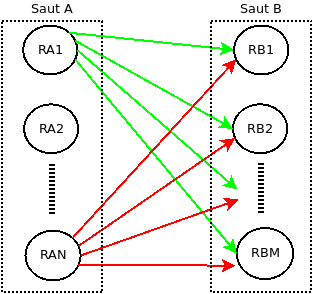
\includegraphics[width=0.5\linewidth]{illustrations/link-inference}
		% Graphic for TeX using PGF
% Title: /home/hayat/RipeAtlasTraceroutesAnalysis/report/illustrations/link-inference.dia
% Creator: Dia v0.97+git
% CreationDate: Thu Nov 29 20:58:09 2018
% For: hayat
% \usepackage{tikz}
% The following commands are not supported in PSTricks at present
% We define them conditionally, so when they are implemented,
% this pgf file will use them.
\ifx\du\undefined
  \newlength{\du}
\fi
\setlength{\du}{15\unitlength}
\begin{tikzpicture}[even odd rule]
\pgftransformxscale{1.000000}
\pgftransformyscale{-1.000000}
\definecolor{dialinecolor}{rgb}{0.000000, 0.000000, 0.000000}
\pgfsetstrokecolor{dialinecolor}
\pgfsetstrokeopacity{1.000000}
\definecolor{diafillcolor}{rgb}{1.000000, 1.000000, 1.000000}
\pgfsetfillcolor{diafillcolor}
\pgfsetfillopacity{1.000000}
\pgfsetlinewidth{0.100000\du}
\pgfsetdash{}{0pt}
\pgfsetmiterjoin
\definecolor{diafillcolor}{rgb}{1.000000, 1.000000, 1.000000}
\pgfsetfillcolor{diafillcolor}
\pgfsetfillopacity{1.000000}
\pgfpathellipse{\pgfpoint{27.430614\du}{13.298442\du}}{\pgfpoint{1.349214\du}{0\du}}{\pgfpoint{0\du}{1.217042\du}}
\pgfusepath{fill}
\definecolor{dialinecolor}{rgb}{0.000000, 0.000000, 0.000000}
\pgfsetstrokecolor{dialinecolor}
\pgfsetstrokeopacity{1.000000}
\pgfpathellipse{\pgfpoint{27.430614\du}{13.298442\du}}{\pgfpoint{1.349214\du}{0\du}}{\pgfpoint{0\du}{1.217042\du}}
\pgfusepath{stroke}
% setfont left to latex
\definecolor{dialinecolor}{rgb}{0.000000, 0.000000, 0.000000}
\pgfsetstrokecolor{dialinecolor}
\pgfsetstrokeopacity{1.000000}
\definecolor{diafillcolor}{rgb}{0.000000, 0.000000, 0.000000}
\pgfsetfillcolor{diafillcolor}
\pgfsetfillopacity{1.000000}
\node[anchor=base,inner sep=0pt, outer sep=0pt,color=dialinecolor] at (27.430614\du,13.493442\du){$R_{1,1}$};
\pgfsetlinewidth{0.100000\du}
\pgfsetdash{}{0pt}
\pgfsetmiterjoin
\definecolor{diafillcolor}{rgb}{1.000000, 1.000000, 1.000000}
\pgfsetfillcolor{diafillcolor}
\pgfsetfillopacity{1.000000}
\pgfpathellipse{\pgfpoint{27.475614\du}{17.238442\du}}{\pgfpoint{1.349214\du}{0\du}}{\pgfpoint{0\du}{1.217042\du}}
\pgfusepath{fill}
\definecolor{dialinecolor}{rgb}{0.000000, 0.000000, 0.000000}
\pgfsetstrokecolor{dialinecolor}
\pgfsetstrokeopacity{1.000000}
\pgfpathellipse{\pgfpoint{27.475614\du}{17.238442\du}}{\pgfpoint{1.349214\du}{0\du}}{\pgfpoint{0\du}{1.217042\du}}
\pgfusepath{stroke}
% setfont left to latex
\definecolor{dialinecolor}{rgb}{0.000000, 0.000000, 0.000000}
\pgfsetstrokecolor{dialinecolor}
\pgfsetstrokeopacity{1.000000}
\definecolor{diafillcolor}{rgb}{0.000000, 0.000000, 0.000000}
\pgfsetfillcolor{diafillcolor}
\pgfsetfillopacity{1.000000}
\node[anchor=base,inner sep=0pt, outer sep=0pt,color=dialinecolor] at (27.475614\du,17.433442\du){$R_{1,2}$};
\pgfsetlinewidth{0.100000\du}
\pgfsetdash{}{0pt}
\pgfsetmiterjoin
\definecolor{diafillcolor}{rgb}{1.000000, 1.000000, 1.000000}
\pgfsetfillcolor{diafillcolor}
\pgfsetfillopacity{1.000000}
\pgfpathellipse{\pgfpoint{27.570578\du}{23.578496\du}}{\pgfpoint{1.376878\du}{0\du}}{\pgfpoint{0\du}{1.241996\du}}
\pgfusepath{fill}
\definecolor{dialinecolor}{rgb}{0.000000, 0.000000, 0.000000}
\pgfsetstrokecolor{dialinecolor}
\pgfsetstrokeopacity{1.000000}
\pgfpathellipse{\pgfpoint{27.570578\du}{23.578496\du}}{\pgfpoint{1.376878\du}{0\du}}{\pgfpoint{0\du}{1.241996\du}}
\pgfusepath{stroke}
% setfont left to latex
\definecolor{dialinecolor}{rgb}{0.000000, 0.000000, 0.000000}
\pgfsetstrokecolor{dialinecolor}
\pgfsetstrokeopacity{1.000000}
\definecolor{diafillcolor}{rgb}{0.000000, 0.000000, 0.000000}
\pgfsetfillcolor{diafillcolor}
\pgfsetfillopacity{1.000000}
\node[anchor=base,inner sep=0pt, outer sep=0pt,color=dialinecolor] at (27.570578\du,23.773496\du){$R_{1,N}$};
\pgfsetlinewidth{0.300000\du}
\pgfsetdash{{\pgflinewidth}{0.200000\du}}{0cm}
\pgfsetbuttcap
{
\definecolor{diafillcolor}{rgb}{0.000000, 0.000000, 0.000000}
\pgfsetfillcolor{diafillcolor}
\pgfsetfillopacity{1.000000}
% was here!!!
\definecolor{dialinecolor}{rgb}{0.000000, 0.000000, 0.000000}
\pgfsetstrokecolor{dialinecolor}
\pgfsetstrokeopacity{1.000000}
\draw (27.540000\du,18.980000\du)--(27.540000\du,21.480000\du);
}
\pgfsetlinewidth{0.100000\du}
\pgfsetdash{}{0pt}
\pgfsetmiterjoin
\definecolor{diafillcolor}{rgb}{1.000000, 1.000000, 1.000000}
\pgfsetfillcolor{diafillcolor}
\pgfsetfillopacity{1.000000}
\pgfpathellipse{\pgfpoint{37.980536\du}{13.298484\du}}{\pgfpoint{1.355136\du}{0\du}}{\pgfpoint{0\du}{1.222384\du}}
\pgfusepath{fill}
\definecolor{dialinecolor}{rgb}{0.000000, 0.000000, 0.000000}
\pgfsetstrokecolor{dialinecolor}
\pgfsetstrokeopacity{1.000000}
\pgfpathellipse{\pgfpoint{37.980536\du}{13.298484\du}}{\pgfpoint{1.355136\du}{0\du}}{\pgfpoint{0\du}{1.222384\du}}
\pgfusepath{stroke}
% setfont left to latex
\definecolor{dialinecolor}{rgb}{0.000000, 0.000000, 0.000000}
\pgfsetstrokecolor{dialinecolor}
\pgfsetstrokeopacity{1.000000}
\definecolor{diafillcolor}{rgb}{0.000000, 0.000000, 0.000000}
\pgfsetfillcolor{diafillcolor}
\pgfsetfillopacity{1.000000}
\node[anchor=base,inner sep=0pt, outer sep=0pt,color=dialinecolor] at (37.980536\du,13.493484\du){$R_{2,1}$};
\pgfsetlinewidth{0.100000\du}
\pgfsetdash{}{0pt}
\pgfsetmiterjoin
\definecolor{diafillcolor}{rgb}{1.000000, 1.000000, 1.000000}
\pgfsetfillcolor{diafillcolor}
\pgfsetfillopacity{1.000000}
\pgfpathellipse{\pgfpoint{37.925536\du}{17.238484\du}}{\pgfpoint{1.355136\du}{0\du}}{\pgfpoint{0\du}{1.222384\du}}
\pgfusepath{fill}
\definecolor{dialinecolor}{rgb}{0.000000, 0.000000, 0.000000}
\pgfsetstrokecolor{dialinecolor}
\pgfsetstrokeopacity{1.000000}
\pgfpathellipse{\pgfpoint{37.925536\du}{17.238484\du}}{\pgfpoint{1.355136\du}{0\du}}{\pgfpoint{0\du}{1.222384\du}}
\pgfusepath{stroke}
% setfont left to latex
\definecolor{dialinecolor}{rgb}{0.000000, 0.000000, 0.000000}
\pgfsetstrokecolor{dialinecolor}
\pgfsetstrokeopacity{1.000000}
\definecolor{diafillcolor}{rgb}{0.000000, 0.000000, 0.000000}
\pgfsetfillcolor{diafillcolor}
\pgfsetfillopacity{1.000000}
\node[anchor=base,inner sep=0pt, outer sep=0pt,color=dialinecolor] at (37.925536\du,17.433484\du){$R_{2,2}$};
\pgfsetlinewidth{0.100000\du}
\pgfsetdash{}{0pt}
\pgfsetmiterjoin
\definecolor{diafillcolor}{rgb}{1.000000, 1.000000, 1.000000}
\pgfsetfillcolor{diafillcolor}
\pgfsetfillopacity{1.000000}
\pgfpathellipse{\pgfpoint{38.170599\du}{23.478445\du}}{\pgfpoint{1.411299\du}{0\du}}{\pgfpoint{0\du}{1.273045\du}}
\pgfusepath{fill}
\definecolor{dialinecolor}{rgb}{0.000000, 0.000000, 0.000000}
\pgfsetstrokecolor{dialinecolor}
\pgfsetstrokeopacity{1.000000}
\pgfpathellipse{\pgfpoint{38.170599\du}{23.478445\du}}{\pgfpoint{1.411299\du}{0\du}}{\pgfpoint{0\du}{1.273045\du}}
\pgfusepath{stroke}
% setfont left to latex
\definecolor{dialinecolor}{rgb}{0.000000, 0.000000, 0.000000}
\pgfsetstrokecolor{dialinecolor}
\pgfsetstrokeopacity{1.000000}
\definecolor{diafillcolor}{rgb}{0.000000, 0.000000, 0.000000}
\pgfsetfillcolor{diafillcolor}
\pgfsetfillopacity{1.000000}
\node[anchor=base,inner sep=0pt, outer sep=0pt,color=dialinecolor] at (38.170599\du,23.673445\du){$R_{1,M}$};
\pgfsetlinewidth{0.300000\du}
\pgfsetdash{{\pgflinewidth}{0.200000\du}}{0cm}
\pgfsetbuttcap
{
\definecolor{diafillcolor}{rgb}{0.000000, 0.000000, 0.000000}
\pgfsetfillcolor{diafillcolor}
\pgfsetfillopacity{1.000000}
% was here!!!
\definecolor{dialinecolor}{rgb}{0.000000, 0.000000, 0.000000}
\pgfsetstrokecolor{dialinecolor}
\pgfsetstrokeopacity{1.000000}
\draw (37.985000\du,18.970000\du)--(37.985000\du,21.470000\du);
}
\pgfsetlinewidth{0.050000\du}
\pgfsetdash{}{0pt}
\pgfsetbuttcap
{
\definecolor{diafillcolor}{rgb}{0.000000, 1.000000, 0.000000}
\pgfsetfillcolor{diafillcolor}
\pgfsetfillopacity{1.000000}
% was here!!!
\pgfsetarrowsstart{stealth}
\definecolor{dialinecolor}{rgb}{0.000000, 1.000000, 0.000000}
\pgfsetstrokecolor{dialinecolor}
\pgfsetstrokeopacity{1.000000}
\draw (28.384600\du,12.437900\du)--(37.022310\du,12.434128\du);
}
\pgfsetlinewidth{0.050000\du}
\pgfsetdash{}{0pt}
\pgfsetbuttcap
{
\definecolor{diafillcolor}{rgb}{1.000000, 0.000000, 0.000000}
\pgfsetfillcolor{diafillcolor}
\pgfsetfillopacity{1.000000}
% was here!!!
\pgfsetarrowsstart{stealth}
\definecolor{dialinecolor}{rgb}{1.000000, 0.000000, 0.000000}
\pgfsetstrokecolor{dialinecolor}
\pgfsetstrokeopacity{1.000000}
\draw (28.842600\du,24.053700\du)--(37.630518\du,24.654584\du);
}
\pgfsetlinewidth{0.100000\du}
\pgfsetdash{{\pgflinewidth}{0.200000\du}}{0cm}
\pgfsetmiterjoin
\pgfsetbuttcap
{\pgfsetcornersarced{\pgfpoint{0.000000\du}{0.000000\du}}\definecolor{dialinecolor}{rgb}{0.000000, 0.000000, 0.000000}
\pgfsetstrokecolor{dialinecolor}
\pgfsetstrokeopacity{1.000000}
\draw (25.638764\du,11.830038\du)--(25.638764\du,25.156536\du)--(29.721269\du,25.156536\du)--(29.721269\du,11.830038\du)--cycle;
}\pgfsetlinewidth{0.100000\du}
\pgfsetdash{{\pgflinewidth}{0.200000\du}}{0cm}
\pgfsetmiterjoin
\pgfsetbuttcap
{\pgfsetcornersarced{\pgfpoint{0.000000\du}{0.000000\du}}\definecolor{dialinecolor}{rgb}{0.000000, 0.000000, 0.000000}
\pgfsetstrokecolor{dialinecolor}
\pgfsetstrokeopacity{1.000000}
\draw (36.096688\du,11.857262\du)--(36.096688\du,25.128574\du)--(39.871607\du,25.128574\du)--(39.871607\du,11.857262\du)--cycle;
}% setfont left to latex
\definecolor{dialinecolor}{rgb}{0.000000, 0.000000, 0.000000}
\pgfsetstrokecolor{dialinecolor}
\pgfsetstrokeopacity{1.000000}
\definecolor{diafillcolor}{rgb}{0.000000, 0.000000, 0.000000}
\pgfsetfillcolor{diafillcolor}
\pgfsetfillopacity{1.000000}
\node[anchor=base west,inner sep=0pt,outer sep=0pt,color=dialinecolor] at (26.470600\du,11.464400\du){$ h_1 $};
% setfont left to latex
\definecolor{dialinecolor}{rgb}{0.000000, 0.000000, 0.000000}
\pgfsetstrokecolor{dialinecolor}
\pgfsetstrokeopacity{1.000000}
\definecolor{diafillcolor}{rgb}{0.000000, 0.000000, 0.000000}
\pgfsetfillcolor{diafillcolor}
\pgfsetfillopacity{1.000000}
\node[anchor=base west,inner sep=0pt,outer sep=0pt,color=dialinecolor] at (36.898700\du,11.464100\du){$ h_2 $};
\pgfsetlinewidth{0.050000\du}
\pgfsetdash{}{0pt}
\pgfsetbuttcap
{
\definecolor{diafillcolor}{rgb}{0.000000, 0.000000, 1.000000}
\pgfsetfillcolor{diafillcolor}
\pgfsetfillopacity{1.000000}
% was here!!!
\pgfsetarrowsstart{stealth}
\definecolor{dialinecolor}{rgb}{0.000000, 0.000000, 1.000000}
\pgfsetstrokecolor{dialinecolor}
\pgfsetstrokeopacity{1.000000}
\draw (28.779828\du,13.298442\du)--(37.406948\du,16.109148\du);
}
\pgfsetlinewidth{0.050000\du}
\pgfsetdash{}{0pt}
\pgfsetbuttcap
{
\definecolor{diafillcolor}{rgb}{0.000000, 1.000000, 0.000000}
\pgfsetfillcolor{diafillcolor}
\pgfsetfillopacity{1.000000}
% was here!!!
\pgfsetarrowsstart{stealth}
\definecolor{dialinecolor}{rgb}{0.000000, 1.000000, 0.000000}
\pgfsetstrokecolor{dialinecolor}
\pgfsetstrokeopacity{1.000000}
\draw (28.722125\du,16.772700\du)--(36.728554\du,12.830698\du);
}
\pgfsetlinewidth{0.050000\du}
\pgfsetdash{}{0pt}
\pgfsetbuttcap
{
\definecolor{diafillcolor}{rgb}{0.000000, 1.000000, 0.000000}
\pgfsetfillcolor{diafillcolor}
\pgfsetfillopacity{1.000000}
% was here!!!
\pgfsetarrowsstart{stealth}
\definecolor{dialinecolor}{rgb}{0.000000, 1.000000, 0.000000}
\pgfsetstrokecolor{dialinecolor}
\pgfsetstrokeopacity{1.000000}
\draw (28.602774\du,20.095348\du)--(36.625400\du,13.298484\du);
}
\pgfsetlinewidth{0.050000\du}
\pgfsetdash{}{0pt}
\pgfsetbuttcap
{
\definecolor{diafillcolor}{rgb}{0.000000, 1.000000, 0.000000}
\pgfsetfillcolor{diafillcolor}
\pgfsetfillopacity{1.000000}
% was here!!!
\pgfsetarrowsstart{stealth}
\definecolor{dialinecolor}{rgb}{0.000000, 1.000000, 0.000000}
\pgfsetstrokecolor{dialinecolor}
\pgfsetstrokeopacity{1.000000}
\draw (28.097487\du,22.431041\du)--(36.728554\du,13.766270\du);
}
\pgfsetlinewidth{0.050000\du}
\pgfsetdash{}{0pt}
\pgfsetbuttcap
{
\definecolor{diafillcolor}{rgb}{0.000000, 0.000000, 1.000000}
\pgfsetfillcolor{diafillcolor}
\pgfsetfillopacity{1.000000}
% was here!!!
\pgfsetarrowsstart{stealth}
\definecolor{dialinecolor}{rgb}{0.000000, 0.000000, 1.000000}
\pgfsetstrokecolor{dialinecolor}
\pgfsetstrokeopacity{1.000000}
\draw (28.824828\du,17.238442\du)--(36.967310\du,16.374128\du);
}
\pgfsetlinewidth{0.050000\du}
\pgfsetdash{}{0pt}
\pgfsetbuttcap
{
\definecolor{diafillcolor}{rgb}{0.000000, 0.000000, 1.000000}
\pgfsetfillcolor{diafillcolor}
\pgfsetfillopacity{1.000000}
% was here!!!
\pgfsetarrowsstart{stealth}
\definecolor{dialinecolor}{rgb}{0.000000, 0.000000, 1.000000}
\pgfsetstrokecolor{dialinecolor}
\pgfsetstrokeopacity{1.000000}
\draw (28.798511\du,20.486821\du)--(36.673554\du,16.770698\du);
}
\pgfsetlinewidth{0.050000\du}
\pgfsetdash{}{0pt}
\pgfsetbuttcap
{
\definecolor{diafillcolor}{rgb}{0.000000, 0.000000, 1.000000}
\pgfsetfillcolor{diafillcolor}
\pgfsetfillopacity{1.000000}
% was here!!!
\pgfsetarrowsstart{stealth}
\definecolor{dialinecolor}{rgb}{0.000000, 0.000000, 1.000000}
\pgfsetstrokecolor{dialinecolor}
\pgfsetstrokeopacity{1.000000}
\draw (28.544178\du,22.700272\du)--(36.516123\du,17.355037\du);
}
\pgfsetlinewidth{0.050000\du}
\pgfsetdash{}{0pt}
\pgfsetbuttcap
{
\definecolor{diafillcolor}{rgb}{1.000000, 0.000000, 0.000000}
\pgfsetfillcolor{diafillcolor}
\pgfsetfillopacity{1.000000}
% was here!!!
\pgfsetarrowsstart{stealth}
\definecolor{dialinecolor}{rgb}{1.000000, 0.000000, 0.000000}
\pgfsetstrokecolor{dialinecolor}
\pgfsetstrokeopacity{1.000000}
\draw (28.938323\du,20.850332\du)--(36.866729\du,23.965618\du);
}
\pgfsetlinewidth{0.050000\du}
\pgfsetdash{}{0pt}
\pgfsetbuttcap
{
\definecolor{diafillcolor}{rgb}{1.000000, 0.000000, 0.000000}
\pgfsetfillcolor{diafillcolor}
\pgfsetfillopacity{1.000000}
% was here!!!
\pgfsetarrowsstart{stealth}
\definecolor{dialinecolor}{rgb}{1.000000, 0.000000, 0.000000}
\pgfsetstrokecolor{dialinecolor}
\pgfsetstrokeopacity{1.000000}
\draw (28.722125\du,17.704183\du)--(36.712688\du,23.381227\du);
}
\pgfsetlinewidth{0.050000\du}
\pgfsetdash{}{0pt}
\pgfsetbuttcap
{
\definecolor{diafillcolor}{rgb}{1.000000, 0.000000, 0.000000}
\pgfsetfillcolor{diafillcolor}
\pgfsetfillopacity{1.000000}
% was here!!!
\pgfsetarrowsstart{stealth}
\definecolor{dialinecolor}{rgb}{1.000000, 0.000000, 0.000000}
\pgfsetstrokecolor{dialinecolor}
\pgfsetstrokeopacity{1.000000}
\draw (28.677125\du,13.764183\du)--(36.866729\du,22.991272\du);
}
\end{tikzpicture}

	}
	\caption{Inférence des liens possibles entre les routeurs des deux sauts $h_{1}$ et $h_{2}$}
	\label{fig:link-inference_}
\end{figure}
\paragraph{5. Calcul des RTTs différentiels des liens.}  A cette étape, on calcule le RTT différentiel de chaque  lien, au sein d'un traceroute donné, en calculant la différence entre les RTTs des deux routeurs impliqués dans le  lien en question (équation \ref{eq:rttdifference}). En plus du RTT différentiel, on note aussi la sonde  ayant effectué la requête traceroute où le lien a été identifié. 

\paragraph{6. Fusion des informations d'un lien.} Un lien (IP1, IP2) peut être identifié plusieurs fois pendant une même période $d_k$. De plus, d'après le travail de référence,  le lien (IP2, IP1) est similaire au lien  (IP1, IP2). La fusion permet de construire une nouvelle distribution des RTTs différentiels caractérisant le lien (IP1, IP2) qui reprend les RTTs différentiels du lien (IP1, IP2) ainsi que ceux du lien (IP2, IP1). Dans le travail de référence, la similarité de deux liens  implique que les RTTs différentiels qui caractérisent un lien (IP2, IP1) caractérisent aussi le lien (IP1, IP2), d'où la fusion effectuée.


A la fin de l'étape 6, tous les traceroutes sont préparés. A présent, l'objectif est d'identifier les dates pendant lesquelles des anomalies ont été détectées. Pour ce faire, l'idée du travail de référence est de conserver, pour un lien donné, une référence du RTT différentiel médian.  Cette référence est d'abord comparée avec la médiane courante des RTTs différentiels,  puis,  mise à jour au fur et à mesure   tout au long de la période de l'analyse. A cette médiane, un intervalle de confiance est associé. Ainsi, l'intervalle de confiance fait partie aussi de la référence du lien. 


\paragraph{7. Calcul de la médiane des RTTs différentiels et  de l'intervalle de confiance courant.} Pour un lien donné, on calcule la médiane des RTTs différentiels d'une $d_k$, ensuite on calcule les deux bornes de l'intervalle de confiance  courant de cette médiane pour ce $d_k$.  



\paragraph{8. Mise à jour de la médiane et de l'intervalle  de confiance de  référence du lien analysé.} La médiane des RTTs différentiels de référence ainsi que l'intervalle de confiance de référence sont mise à jour tant que la période déclenchant la détection des anomalies n'est pas atteinte.  La mise à jour de la référence : médiane et les bornes de l'intervalle de confiance se base sur la moyenne mobile exponentielle. Cette méthode prend en compte les valeurs antérieures ainsi que celles récentes en étant dirigée par le paramètre \textit{confInterval} décrit dans la section \ref{par:parametre-de-lanalyse}.


\paragraph{9. Comparaison des intervalles de confiance.} 

La comparaison de l'état courant du lien avec celui de référence est effectuée en analysant le chevauchement d'intervalles de confiance  courant et de référence. Le délai d'un lien est jugé normal si son intervalle de confiance courant est inclus dans l'intervalle de confiance de référence. C'est le cas $1$ dans la Figure 	\ref{fig:intervals-comparaison},  \textit{referenceLow} et \textit{referenceHight} sont les bornes de l'intervalle de confiance de référence.  \textit{currentLow} et \textit{currentHight} sont les bornes de l'intervalle de confiance courant.
D'après le travail de référence, on distingue quatre cas possibles  illustrés dans la Figure 	\ref{fig:intervals-comparaison}:

\textbf{Cas 1 :} le délai du lien est normal.

\textbf{Cas 2 :} le délai du lien est anormal.

\textbf{Cas 3 :} le délai du lien est anormal.

\textbf{Cas 4 :} le délai du lien est anormal.

Dans le cas où le délai est jugé anormal, on introduit ce qu'on appelle la \textit{déviation}. Cette métrique caractérise l'anomalie détectée. Elle est calculée différemment dans le cas où le délai est anormal.

\begin{figure}[h]
	\centering
	\captionsetup{justification=centering}
	\resizebox{\textwidth}{!}{
		% Graphic for TeX using PGF
% Title: /home/hayat/RipeAtlasTraceroutesAnalysis/report/illustrations/intervals-comparaison.dia
% Creator: Dia v0.97+git
% CreationDate: Tue Dec  4 13:30:20 2018
% For: hayat
% \usepackage{tikz}
% The following commands are not supported in PSTricks at present
% We define them conditionally, so when they are implemented,
% this pgf file will use them.
\ifx\du\undefined
  \newlength{\du}
\fi
\setlength{\du}{15\unitlength}
\begin{tikzpicture}[even odd rule]
\pgftransformxscale{1.000000}
\pgftransformyscale{-1.000000}
\definecolor{dialinecolor}{rgb}{0.000000, 0.000000, 0.000000}
\pgfsetstrokecolor{dialinecolor}
\pgfsetstrokeopacity{1.000000}
\definecolor{diafillcolor}{rgb}{1.000000, 1.000000, 1.000000}
\pgfsetfillcolor{diafillcolor}
\pgfsetfillopacity{1.000000}
\pgfsetlinewidth{0.100000\du}
\pgfsetdash{}{0pt}
\pgfsetbuttcap
{
\definecolor{diafillcolor}{rgb}{0.662745, 0.709804, 0.674510}
\pgfsetfillcolor{diafillcolor}
\pgfsetfillopacity{1.000000}
% was here!!!
}
\definecolor{dialinecolor}{rgb}{0.662745, 0.709804, 0.674510}
\pgfsetstrokecolor{dialinecolor}
\pgfsetstrokeopacity{1.000000}
\draw (14.150000\du,0.400000\du)--(27.000000\du,0.400000\du);
\pgfsetlinewidth{0.100000\du}
\pgfsetdash{}{0pt}
\pgfsetmiterjoin
\pgfsetbuttcap
\definecolor{diafillcolor}{rgb}{0.662745, 0.709804, 0.674510}
\pgfsetfillcolor{diafillcolor}
\pgfsetfillopacity{1.000000}
\fill (13.900000\du,0.550000\du)--(13.900000\du,0.250000\du)--(14.200000\du,0.250000\du)--(14.200000\du,0.550000\du)--cycle;
\definecolor{dialinecolor}{rgb}{0.662745, 0.709804, 0.674510}
\pgfsetstrokecolor{dialinecolor}
\pgfsetstrokeopacity{1.000000}
\draw (14.050000\du,0.700000\du)--(14.050000\du,0.100000\du);
\pgfsetlinewidth{0.100000\du}
\pgfsetdash{}{0pt}
\pgfsetmiterjoin
\pgfsetbuttcap
\definecolor{diafillcolor}{rgb}{0.662745, 0.709804, 0.674510}
\pgfsetfillcolor{diafillcolor}
\pgfsetfillopacity{1.000000}
\fill (27.250000\du,0.250000\du)--(27.250000\du,0.550000\du)--(26.950000\du,0.550000\du)--(26.950000\du,0.250000\du)--cycle;
\definecolor{dialinecolor}{rgb}{0.662745, 0.709804, 0.674510}
\pgfsetstrokecolor{dialinecolor}
\pgfsetstrokeopacity{1.000000}
\draw (27.100000\du,0.100000\du)--(27.100000\du,0.700000\du);
\pgfsetlinewidth{0.100000\du}
\pgfsetdash{}{0pt}
\pgfsetbuttcap
{
\definecolor{diafillcolor}{rgb}{0.000000, 0.000000, 0.000000}
\pgfsetfillcolor{diafillcolor}
\pgfsetfillopacity{1.000000}
% was here!!!
}
\definecolor{dialinecolor}{rgb}{0.000000, 0.000000, 0.000000}
\pgfsetstrokecolor{dialinecolor}
\pgfsetstrokeopacity{1.000000}
\draw (16.150000\du,2.450000\du)--(24.800000\du,2.450000\du);
\pgfsetlinewidth{0.100000\du}
\pgfsetdash{}{0pt}
\pgfsetmiterjoin
\pgfsetbuttcap
\definecolor{diafillcolor}{rgb}{0.000000, 0.000000, 0.000000}
\pgfsetfillcolor{diafillcolor}
\pgfsetfillopacity{1.000000}
\fill (15.900000\du,2.600000\du)--(15.900000\du,2.300000\du)--(16.200000\du,2.300000\du)--(16.200000\du,2.600000\du)--cycle;
\definecolor{dialinecolor}{rgb}{0.000000, 0.000000, 0.000000}
\pgfsetstrokecolor{dialinecolor}
\pgfsetstrokeopacity{1.000000}
\draw (16.050000\du,2.750000\du)--(16.050000\du,2.150000\du);
\pgfsetlinewidth{0.100000\du}
\pgfsetdash{}{0pt}
\pgfsetmiterjoin
\pgfsetbuttcap
\definecolor{diafillcolor}{rgb}{0.000000, 0.000000, 0.000000}
\pgfsetfillcolor{diafillcolor}
\pgfsetfillopacity{1.000000}
\fill (25.050000\du,2.300000\du)--(25.050000\du,2.600000\du)--(24.750000\du,2.600000\du)--(24.750000\du,2.300000\du)--cycle;
\definecolor{dialinecolor}{rgb}{0.000000, 0.000000, 0.000000}
\pgfsetstrokecolor{dialinecolor}
\pgfsetstrokeopacity{1.000000}
\draw (24.900000\du,2.150000\du)--(24.900000\du,2.750000\du);
\pgfsetlinewidth{0.100000\du}
\pgfsetdash{}{0pt}
\pgfsetbuttcap
{
\definecolor{diafillcolor}{rgb}{0.662745, 0.709804, 0.674510}
\pgfsetfillcolor{diafillcolor}
\pgfsetfillopacity{1.000000}
% was here!!!
}
\definecolor{dialinecolor}{rgb}{0.662745, 0.709804, 0.674510}
\pgfsetstrokecolor{dialinecolor}
\pgfsetstrokeopacity{1.000000}
\draw (14.008246\du,11.548114\du)--(26.858246\du,11.548114\du);
\pgfsetlinewidth{0.100000\du}
\pgfsetdash{}{0pt}
\pgfsetmiterjoin
\pgfsetbuttcap
\definecolor{diafillcolor}{rgb}{0.662745, 0.709804, 0.674510}
\pgfsetfillcolor{diafillcolor}
\pgfsetfillopacity{1.000000}
\fill (13.758246\du,11.698114\du)--(13.758246\du,11.398114\du)--(14.058246\du,11.398114\du)--(14.058246\du,11.698114\du)--cycle;
\definecolor{dialinecolor}{rgb}{0.662745, 0.709804, 0.674510}
\pgfsetstrokecolor{dialinecolor}
\pgfsetstrokeopacity{1.000000}
\draw (13.908246\du,11.848114\du)--(13.908246\du,11.248114\du);
\pgfsetlinewidth{0.100000\du}
\pgfsetdash{}{0pt}
\pgfsetmiterjoin
\pgfsetbuttcap
\definecolor{diafillcolor}{rgb}{0.662745, 0.709804, 0.674510}
\pgfsetfillcolor{diafillcolor}
\pgfsetfillopacity{1.000000}
\fill (27.108246\du,11.398114\du)--(27.108246\du,11.698114\du)--(26.808246\du,11.698114\du)--(26.808246\du,11.398114\du)--cycle;
\definecolor{dialinecolor}{rgb}{0.662745, 0.709804, 0.674510}
\pgfsetstrokecolor{dialinecolor}
\pgfsetstrokeopacity{1.000000}
\draw (26.958246\du,11.248114\du)--(26.958246\du,11.848114\du);
\pgfsetlinewidth{0.100000\du}
\pgfsetdash{}{0pt}
\pgfsetbuttcap
{
\definecolor{diafillcolor}{rgb}{0.000000, 0.000000, 0.000000}
\pgfsetfillcolor{diafillcolor}
\pgfsetfillopacity{1.000000}
% was here!!!
}
\definecolor{dialinecolor}{rgb}{0.000000, 0.000000, 0.000000}
\pgfsetstrokecolor{dialinecolor}
\pgfsetstrokeopacity{1.000000}
\draw (23.108246\du,13.598114\du)--(31.758246\du,13.598114\du);
\pgfsetlinewidth{0.100000\du}
\pgfsetdash{}{0pt}
\pgfsetmiterjoin
\pgfsetbuttcap
\definecolor{diafillcolor}{rgb}{0.000000, 0.000000, 0.000000}
\pgfsetfillcolor{diafillcolor}
\pgfsetfillopacity{1.000000}
\fill (22.858246\du,13.748114\du)--(22.858246\du,13.448114\du)--(23.158246\du,13.448114\du)--(23.158246\du,13.748114\du)--cycle;
\definecolor{dialinecolor}{rgb}{0.000000, 0.000000, 0.000000}
\pgfsetstrokecolor{dialinecolor}
\pgfsetstrokeopacity{1.000000}
\draw (23.008246\du,13.898114\du)--(23.008246\du,13.298114\du);
\pgfsetlinewidth{0.100000\du}
\pgfsetdash{}{0pt}
\pgfsetmiterjoin
\pgfsetbuttcap
\definecolor{diafillcolor}{rgb}{0.000000, 0.000000, 0.000000}
\pgfsetfillcolor{diafillcolor}
\pgfsetfillopacity{1.000000}
\fill (32.008246\du,13.448114\du)--(32.008246\du,13.748114\du)--(31.708246\du,13.748114\du)--(31.708246\du,13.448114\du)--cycle;
\definecolor{dialinecolor}{rgb}{0.000000, 0.000000, 0.000000}
\pgfsetstrokecolor{dialinecolor}
\pgfsetstrokeopacity{1.000000}
\draw (31.858246\du,13.298114\du)--(31.858246\du,13.898114\du);
\pgfsetlinewidth{0.100000\du}
\pgfsetdash{}{0pt}
\pgfsetbuttcap
{
\definecolor{diafillcolor}{rgb}{0.662745, 0.709804, 0.674510}
\pgfsetfillcolor{diafillcolor}
\pgfsetfillopacity{1.000000}
% was here!!!
}
\definecolor{dialinecolor}{rgb}{0.662745, 0.709804, 0.674510}
\pgfsetstrokecolor{dialinecolor}
\pgfsetstrokeopacity{1.000000}
\draw (14.108246\du,17.048114\du)--(26.958246\du,17.048114\du);
\pgfsetlinewidth{0.100000\du}
\pgfsetdash{}{0pt}
\pgfsetmiterjoin
\pgfsetbuttcap
\definecolor{diafillcolor}{rgb}{0.662745, 0.709804, 0.674510}
\pgfsetfillcolor{diafillcolor}
\pgfsetfillopacity{1.000000}
\fill (13.858246\du,17.198114\du)--(13.858246\du,16.898114\du)--(14.158246\du,16.898114\du)--(14.158246\du,17.198114\du)--cycle;
\definecolor{dialinecolor}{rgb}{0.662745, 0.709804, 0.674510}
\pgfsetstrokecolor{dialinecolor}
\pgfsetstrokeopacity{1.000000}
\draw (14.008246\du,17.348114\du)--(14.008246\du,16.748114\du);
\pgfsetlinewidth{0.100000\du}
\pgfsetdash{}{0pt}
\pgfsetmiterjoin
\pgfsetbuttcap
\definecolor{diafillcolor}{rgb}{0.662745, 0.709804, 0.674510}
\pgfsetfillcolor{diafillcolor}
\pgfsetfillopacity{1.000000}
\fill (27.208246\du,16.898114\du)--(27.208246\du,17.198114\du)--(26.908246\du,17.198114\du)--(26.908246\du,16.898114\du)--cycle;
\definecolor{dialinecolor}{rgb}{0.662745, 0.709804, 0.674510}
\pgfsetstrokecolor{dialinecolor}
\pgfsetstrokeopacity{1.000000}
\draw (27.058246\du,16.748114\du)--(27.058246\du,17.348114\du);
\pgfsetlinewidth{0.100000\du}
\pgfsetdash{}{0pt}
\pgfsetbuttcap
{
\definecolor{diafillcolor}{rgb}{0.000000, 0.000000, 0.000000}
\pgfsetfillcolor{diafillcolor}
\pgfsetfillopacity{1.000000}
% was here!!!
}
\definecolor{dialinecolor}{rgb}{0.000000, 0.000000, 0.000000}
\pgfsetstrokecolor{dialinecolor}
\pgfsetstrokeopacity{1.000000}
\draw (9.308246\du,19.048114\du)--(17.958246\du,19.048114\du);
\pgfsetlinewidth{0.100000\du}
\pgfsetdash{}{0pt}
\pgfsetmiterjoin
\pgfsetbuttcap
\definecolor{diafillcolor}{rgb}{0.000000, 0.000000, 0.000000}
\pgfsetfillcolor{diafillcolor}
\pgfsetfillopacity{1.000000}
\fill (9.058246\du,19.198114\du)--(9.058246\du,18.898114\du)--(9.358246\du,18.898114\du)--(9.358246\du,19.198114\du)--cycle;
\definecolor{dialinecolor}{rgb}{0.000000, 0.000000, 0.000000}
\pgfsetstrokecolor{dialinecolor}
\pgfsetstrokeopacity{1.000000}
\draw (9.208246\du,19.348114\du)--(9.208246\du,18.748114\du);
\pgfsetlinewidth{0.100000\du}
\pgfsetdash{}{0pt}
\pgfsetmiterjoin
\pgfsetbuttcap
\definecolor{diafillcolor}{rgb}{0.000000, 0.000000, 0.000000}
\pgfsetfillcolor{diafillcolor}
\pgfsetfillopacity{1.000000}
\fill (18.208246\du,18.898114\du)--(18.208246\du,19.198114\du)--(17.908246\du,19.198114\du)--(17.908246\du,18.898114\du)--cycle;
\definecolor{dialinecolor}{rgb}{0.000000, 0.000000, 0.000000}
\pgfsetstrokecolor{dialinecolor}
\pgfsetstrokeopacity{1.000000}
\draw (18.058246\du,18.748114\du)--(18.058246\du,19.348114\du);
\pgfsetlinewidth{0.100000\du}
\pgfsetdash{{\pgflinewidth}{0.200000\du}}{0cm}
\pgfsetbuttcap
{
\definecolor{diafillcolor}{rgb}{0.000000, 0.000000, 0.000000}
\pgfsetfillcolor{diafillcolor}
\pgfsetfillopacity{1.000000}
% was here!!!
\pgfsetarrowsend{stealth}
\definecolor{dialinecolor}{rgb}{0.000000, 0.000000, 0.000000}
\pgfsetstrokecolor{dialinecolor}
\pgfsetstrokeopacity{1.000000}
\draw (5.050000\du,21.000000\du)--(38.800000\du,20.950000\du);
}
\pgfsetlinewidth{0.100000\du}
\pgfsetdash{}{0pt}
\pgfsetbuttcap
{
\definecolor{diafillcolor}{rgb}{0.662745, 0.709804, 0.674510}
\pgfsetfillcolor{diafillcolor}
\pgfsetfillopacity{1.000000}
% was here!!!
}
\definecolor{dialinecolor}{rgb}{0.662745, 0.709804, 0.674510}
\pgfsetstrokecolor{dialinecolor}
\pgfsetstrokeopacity{1.000000}
\draw (13.958246\du,6.048114\du)--(26.808246\du,6.048114\du);
\pgfsetlinewidth{0.100000\du}
\pgfsetdash{}{0pt}
\pgfsetmiterjoin
\pgfsetbuttcap
\definecolor{diafillcolor}{rgb}{0.662745, 0.709804, 0.674510}
\pgfsetfillcolor{diafillcolor}
\pgfsetfillopacity{1.000000}
\fill (13.708246\du,6.198114\du)--(13.708246\du,5.898114\du)--(14.008246\du,5.898114\du)--(14.008246\du,6.198114\du)--cycle;
\definecolor{dialinecolor}{rgb}{0.662745, 0.709804, 0.674510}
\pgfsetstrokecolor{dialinecolor}
\pgfsetstrokeopacity{1.000000}
\draw (13.858246\du,6.348114\du)--(13.858246\du,5.748114\du);
\pgfsetlinewidth{0.100000\du}
\pgfsetdash{}{0pt}
\pgfsetmiterjoin
\pgfsetbuttcap
\definecolor{diafillcolor}{rgb}{0.662745, 0.709804, 0.674510}
\pgfsetfillcolor{diafillcolor}
\pgfsetfillopacity{1.000000}
\fill (27.058246\du,5.898114\du)--(27.058246\du,6.198114\du)--(26.758246\du,6.198114\du)--(26.758246\du,5.898114\du)--cycle;
\definecolor{dialinecolor}{rgb}{0.662745, 0.709804, 0.674510}
\pgfsetstrokecolor{dialinecolor}
\pgfsetstrokeopacity{1.000000}
\draw (26.908246\du,5.748114\du)--(26.908246\du,6.348114\du);
\pgfsetlinewidth{0.100000\du}
\pgfsetdash{}{0pt}
\pgfsetbuttcap
{
\definecolor{diafillcolor}{rgb}{0.000000, 0.000000, 0.000000}
\pgfsetfillcolor{diafillcolor}
\pgfsetfillopacity{1.000000}
% was here!!!
}
\definecolor{dialinecolor}{rgb}{0.000000, 0.000000, 0.000000}
\pgfsetstrokecolor{dialinecolor}
\pgfsetstrokeopacity{1.000000}
\draw (10.049999\du,8.049461\du)--(32.750001\du,8.000539\du);
\pgfsetlinewidth{0.100000\du}
\pgfsetdash{}{0pt}
\pgfsetmiterjoin
\pgfsetbuttcap
\definecolor{diafillcolor}{rgb}{0.000000, 0.000000, 0.000000}
\pgfsetfillcolor{diafillcolor}
\pgfsetfillopacity{1.000000}
\fill (9.800323\du,8.200000\du)--(9.799677\du,7.900000\du)--(10.099676\du,7.899354\du)--(10.100323\du,8.199353\du)--cycle;
\definecolor{dialinecolor}{rgb}{0.000000, 0.000000, 0.000000}
\pgfsetstrokecolor{dialinecolor}
\pgfsetstrokeopacity{1.000000}
\draw (9.950646\du,8.349676\du)--(9.949353\du,7.749677\du);
\pgfsetlinewidth{0.100000\du}
\pgfsetdash{}{0pt}
\pgfsetmiterjoin
\pgfsetbuttcap
\definecolor{diafillcolor}{rgb}{0.000000, 0.000000, 0.000000}
\pgfsetfillcolor{diafillcolor}
\pgfsetfillopacity{1.000000}
\fill (32.999677\du,7.850000\du)--(33.000323\du,8.150000\du)--(32.700324\du,8.150646\du)--(32.699677\du,7.850647\du)--cycle;
\definecolor{dialinecolor}{rgb}{0.000000, 0.000000, 0.000000}
\pgfsetstrokecolor{dialinecolor}
\pgfsetstrokeopacity{1.000000}
\draw (32.849354\du,7.700324\du)--(32.850647\du,8.300323\du);
\pgfsetlinewidth{0.050000\du}
\pgfsetdash{}{0pt}
\pgfsetmiterjoin
\pgfsetbuttcap
{\pgfsetcornersarced{\pgfpoint{0.000000\du}{0.000000\du}}\definecolor{dialinecolor}{rgb}{0.000000, 0.000000, 0.000000}
\pgfsetstrokecolor{dialinecolor}
\pgfsetstrokeopacity{1.000000}
\draw (6.900000\du,4.500000\du)--(6.900000\du,8.950000\du)--(36.950000\du,8.950000\du)--(36.950000\du,4.500000\du)--cycle;
}% setfont left to latex
\definecolor{dialinecolor}{rgb}{0.000000, 0.000000, 0.000000}
\pgfsetstrokecolor{dialinecolor}
\pgfsetstrokeopacity{1.000000}
\definecolor{diafillcolor}{rgb}{0.000000, 0.000000, 0.000000}
\pgfsetfillcolor{diafillcolor}
\pgfsetfillopacity{1.000000}
\node[anchor=base west,inner sep=0pt,outer sep=0pt,color=dialinecolor] at (7.950000\du,7.550000\du){currentLow};
% setfont left to latex
\definecolor{dialinecolor}{rgb}{0.000000, 0.000000, 0.000000}
\pgfsetstrokecolor{dialinecolor}
\pgfsetstrokeopacity{1.000000}
\definecolor{diafillcolor}{rgb}{0.000000, 0.000000, 0.000000}
\pgfsetfillcolor{diafillcolor}
\pgfsetfillopacity{1.000000}
\node[anchor=base west,inner sep=0pt,outer sep=0pt,color=dialinecolor] at (30.800000\du,7.500000\du){currentHight};
% setfont left to latex
\definecolor{dialinecolor}{rgb}{0.282353, 0.313726, 0.290196}
\pgfsetstrokecolor{dialinecolor}
\pgfsetstrokeopacity{1.000000}
\definecolor{diafillcolor}{rgb}{0.282353, 0.313726, 0.290196}
\pgfsetfillcolor{diafillcolor}
\pgfsetfillopacity{1.000000}
\node[anchor=base west,inner sep=0pt,outer sep=0pt,color=dialinecolor] at (11.450000\du,5.550000\du){referenceLow};
% setfont left to latex
\definecolor{dialinecolor}{rgb}{0.282353, 0.313726, 0.290196}
\pgfsetstrokecolor{dialinecolor}
\pgfsetstrokeopacity{1.000000}
\definecolor{diafillcolor}{rgb}{0.282353, 0.313726, 0.290196}
\pgfsetfillcolor{diafillcolor}
\pgfsetfillopacity{1.000000}
\node[anchor=base west,inner sep=0pt,outer sep=0pt,color=dialinecolor] at (23.750000\du,5.550000\du){referenceHight};
% setfont left to latex
\definecolor{dialinecolor}{rgb}{0.282353, 0.313726, 0.290196}
\pgfsetstrokecolor{dialinecolor}
\pgfsetstrokeopacity{1.000000}
\definecolor{diafillcolor}{rgb}{0.282353, 0.313726, 0.290196}
\pgfsetfillcolor{diafillcolor}
\pgfsetfillopacity{1.000000}
\node[anchor=base west,inner sep=0pt,outer sep=0pt,color=dialinecolor] at (24.545000\du,-0.297500\du){referenceHight};
% setfont left to latex
\definecolor{dialinecolor}{rgb}{0.282353, 0.313726, 0.290196}
\pgfsetstrokecolor{dialinecolor}
\pgfsetstrokeopacity{1.000000}
\definecolor{diafillcolor}{rgb}{0.282353, 0.313726, 0.290196}
\pgfsetfillcolor{diafillcolor}
\pgfsetfillopacity{1.000000}
\node[anchor=base west,inner sep=0pt,outer sep=0pt,color=dialinecolor] at (24.390000\du,10.792500\du){referenceHight};
% setfont left to latex
\definecolor{dialinecolor}{rgb}{0.282353, 0.313726, 0.290196}
\pgfsetstrokecolor{dialinecolor}
\pgfsetstrokeopacity{1.000000}
\definecolor{diafillcolor}{rgb}{0.282353, 0.313726, 0.290196}
\pgfsetfillcolor{diafillcolor}
\pgfsetfillopacity{1.000000}
\node[anchor=base west,inner sep=0pt,outer sep=0pt,color=dialinecolor] at (24.485000\du,16.282500\du){referenceHight};
% setfont left to latex
\definecolor{dialinecolor}{rgb}{0.282353, 0.313726, 0.290196}
\pgfsetstrokecolor{dialinecolor}
\pgfsetstrokeopacity{1.000000}
\definecolor{diafillcolor}{rgb}{0.282353, 0.313726, 0.290196}
\pgfsetfillcolor{diafillcolor}
\pgfsetfillopacity{1.000000}
\node[anchor=base west,inner sep=0pt,outer sep=0pt,color=dialinecolor] at (12.045000\du,-0.247500\du){referenceLow};
% setfont left to latex
\definecolor{dialinecolor}{rgb}{0.282353, 0.313726, 0.290196}
\pgfsetstrokecolor{dialinecolor}
\pgfsetstrokeopacity{1.000000}
\definecolor{diafillcolor}{rgb}{0.282353, 0.313726, 0.290196}
\pgfsetfillcolor{diafillcolor}
\pgfsetfillopacity{1.000000}
\node[anchor=base west,inner sep=0pt,outer sep=0pt,color=dialinecolor] at (11.340000\du,10.892500\du){referenceLow};
% setfont left to latex
\definecolor{dialinecolor}{rgb}{0.282353, 0.313726, 0.290196}
\pgfsetstrokecolor{dialinecolor}
\pgfsetstrokeopacity{1.000000}
\definecolor{diafillcolor}{rgb}{0.282353, 0.313726, 0.290196}
\pgfsetfillcolor{diafillcolor}
\pgfsetfillopacity{1.000000}
\node[anchor=base west,inner sep=0pt,outer sep=0pt,color=dialinecolor] at (11.535000\du,16.532500\du){referenceLow};
% setfont left to latex
\definecolor{dialinecolor}{rgb}{0.000000, 0.000000, 0.000000}
\pgfsetstrokecolor{dialinecolor}
\pgfsetstrokeopacity{1.000000}
\definecolor{diafillcolor}{rgb}{0.000000, 0.000000, 0.000000}
\pgfsetfillcolor{diafillcolor}
\pgfsetfillopacity{1.000000}
\node[anchor=base west,inner sep=0pt,outer sep=0pt,color=dialinecolor] at (13.845000\du,2.002500\du){currentLow};
% setfont left to latex
\definecolor{dialinecolor}{rgb}{0.000000, 0.000000, 0.000000}
\pgfsetstrokecolor{dialinecolor}
\pgfsetstrokeopacity{1.000000}
\definecolor{diafillcolor}{rgb}{0.000000, 0.000000, 0.000000}
\pgfsetfillcolor{diafillcolor}
\pgfsetfillopacity{1.000000}
\node[anchor=base west,inner sep=0pt,outer sep=0pt,color=dialinecolor] at (22.745000\du,2.002500\du){currentHight};
\pgfsetlinewidth{0.050000\du}
\pgfsetdash{}{0pt}
\pgfsetmiterjoin
\pgfsetbuttcap
{\pgfsetcornersarced{\pgfpoint{0.000000\du}{0.000000\du}}\definecolor{dialinecolor}{rgb}{0.000000, 0.000000, 0.000000}
\pgfsetstrokecolor{dialinecolor}
\pgfsetstrokeopacity{1.000000}
\draw (7.000000\du,-1.085000\du)--(7.000000\du,3.365000\du)--(37.000000\du,3.365000\du)--(37.000000\du,-1.085000\du)--cycle;
}% setfont left to latex
\definecolor{dialinecolor}{rgb}{0.000000, 0.000000, 0.000000}
\pgfsetstrokecolor{dialinecolor}
\pgfsetstrokeopacity{1.000000}
\definecolor{diafillcolor}{rgb}{0.000000, 0.000000, 0.000000}
\pgfsetfillcolor{diafillcolor}
\pgfsetfillopacity{1.000000}
\node[anchor=base west,inner sep=0pt,outer sep=0pt,color=dialinecolor] at (20.895000\du,13.002500\du){currentLow};
% setfont left to latex
\definecolor{dialinecolor}{rgb}{0.000000, 0.000000, 0.000000}
\pgfsetstrokecolor{dialinecolor}
\pgfsetstrokeopacity{1.000000}
\definecolor{diafillcolor}{rgb}{0.000000, 0.000000, 0.000000}
\pgfsetfillcolor{diafillcolor}
\pgfsetfillopacity{1.000000}
\node[anchor=base west,inner sep=0pt,outer sep=0pt,color=dialinecolor] at (7.140000\du,18.292500\du){currentLow};
% setfont left to latex
\definecolor{dialinecolor}{rgb}{0.000000, 0.000000, 0.000000}
\pgfsetstrokecolor{dialinecolor}
\pgfsetstrokeopacity{1.000000}
\definecolor{diafillcolor}{rgb}{0.000000, 0.000000, 0.000000}
\pgfsetfillcolor{diafillcolor}
\pgfsetfillopacity{1.000000}
\node[anchor=base west,inner sep=0pt,outer sep=0pt,color=dialinecolor] at (29.695000\du,13.002500\du){currentHight};
% setfont left to latex
\definecolor{dialinecolor}{rgb}{0.000000, 0.000000, 0.000000}
\pgfsetstrokecolor{dialinecolor}
\pgfsetstrokeopacity{1.000000}
\definecolor{diafillcolor}{rgb}{0.000000, 0.000000, 0.000000}
\pgfsetfillcolor{diafillcolor}
\pgfsetfillopacity{1.000000}
\node[anchor=base west,inner sep=0pt,outer sep=0pt,color=dialinecolor] at (15.840000\du,18.442500\du){currentHight};
\pgfsetlinewidth{0.050000\du}
\pgfsetdash{}{0pt}
\pgfsetmiterjoin
\pgfsetbuttcap
{\pgfsetcornersarced{\pgfpoint{0.000000\du}{0.000000\du}}\definecolor{dialinecolor}{rgb}{0.000000, 0.000000, 0.000000}
\pgfsetstrokecolor{dialinecolor}
\pgfsetstrokeopacity{1.000000}
\draw (7.000000\du,10.015000\du)--(7.000000\du,14.465000\du)--(37.050000\du,14.465000\du)--(37.050000\du,10.015000\du)--cycle;
}\pgfsetlinewidth{0.050000\du}
\pgfsetdash{}{0pt}
\pgfsetmiterjoin
\pgfsetbuttcap
{\pgfsetcornersarced{\pgfpoint{0.000000\du}{0.000000\du}}\definecolor{dialinecolor}{rgb}{0.000000, 0.000000, 0.000000}
\pgfsetstrokecolor{dialinecolor}
\pgfsetstrokeopacity{1.000000}
\draw (6.950000\du,15.515000\du)--(6.950000\du,19.965000\du)--(37.050000\du,19.965000\du)--(37.050000\du,15.515000\du)--cycle;
}% setfont left to latex
\definecolor{dialinecolor}{rgb}{0.000000, 0.000000, 0.000000}
\pgfsetstrokecolor{dialinecolor}
\pgfsetstrokeopacity{1.000000}
\definecolor{diafillcolor}{rgb}{0.000000, 0.000000, 0.000000}
\pgfsetfillcolor{diafillcolor}
\pgfsetfillopacity{1.000000}
\node[anchor=base west,inner sep=0pt,outer sep=0pt,color=dialinecolor] at (3.950000\du,1.000000\du){Cas 1};
% setfont left to latex
\definecolor{dialinecolor}{rgb}{0.000000, 0.000000, 0.000000}
\pgfsetstrokecolor{dialinecolor}
\pgfsetstrokeopacity{1.000000}
\definecolor{diafillcolor}{rgb}{0.000000, 0.000000, 0.000000}
\pgfsetfillcolor{diafillcolor}
\pgfsetfillopacity{1.000000}
\node[anchor=base west,inner sep=0pt,outer sep=0pt,color=dialinecolor] at (4.050000\du,7.000000\du){Cas 2};
% setfont left to latex
\definecolor{dialinecolor}{rgb}{0.000000, 0.000000, 0.000000}
\pgfsetstrokecolor{dialinecolor}
\pgfsetstrokeopacity{1.000000}
\definecolor{diafillcolor}{rgb}{0.000000, 0.000000, 0.000000}
\pgfsetfillcolor{diafillcolor}
\pgfsetfillopacity{1.000000}
\node[anchor=base west,inner sep=0pt,outer sep=0pt,color=dialinecolor] at (4.050000\du,12.000000\du){Cas 3};
% setfont left to latex
\definecolor{dialinecolor}{rgb}{0.000000, 0.000000, 0.000000}
\pgfsetstrokecolor{dialinecolor}
\pgfsetstrokeopacity{1.000000}
\definecolor{diafillcolor}{rgb}{0.000000, 0.000000, 0.000000}
\pgfsetfillcolor{diafillcolor}
\pgfsetfillopacity{1.000000}
\node[anchor=base west,inner sep=0pt,outer sep=0pt,color=dialinecolor] at (4.050000\du,18.100000\du){Cas 4};
\end{tikzpicture}

	}
	\caption{La comparaison des deux intervalles de confiance : courant et référence }
	\label{fig:intervals-comparaison}
\end{figure}

%Ces étapes sont reprises dans  la Figure \ref{fig:process-rttanalysis_tex}. [!]


\subsection{Processus de détection des anomalies :  notation entrées et sorties} \label{processus-de-detection}
La détection des anomalies dans les délais des liens peut être organisée en deux phases: la préparation de données et la détection des alarmes.
\paragraph{Phase I : préparation de données.}

\begin{itemize}
	\item \textbf{findAllBins (I.1)} : nous cherchons la liste des périodes ({\color{gray}[bin]}) entre  {\color{gray}start} et  {\color{gray}end}. La durée de chaque {\color{gray}bin} vaut  {\color{gray}timeWindow}.
	\item \textbf{findTraceroutesByBin (I.2)} : pour toute période  ({\color{gray}bin}), nous récupérons les traceroutes
	capturés durant cette dernière. Le nombre de traceroutes associés à chaque {\color{gray}bin} dépend
	des traceroutes disponibles à l'analyse  ({\color{gray}[traceroute]}).
	\item \textbf{removeInvalidTraceroutes (I.3)} : certains traceroutes ne réussissent pas à atteindre la destination prévue, dans ce cas, ces traceroutes sont ignorés. De même, les sauts ayant des RTTs invalides
	sont aussi ignorés.
	\item \textbf{aggregateRttsByHop (I.4)} : étant donné que chaque saut  ({\color{gray}hop}) est décrit par plus d'un RTT, nous calculons la médiane de ces RTTs  ({\color{gray}rttAgg}), et ce par source de signal.
	\item \textbf{linkInference (I.5)} : chaque deux sauts consécutifs d'un traceroute forment un lien. Pour
	tout traceroute d'un  {\color{gray}bin} donné, nous déduisons les liens possibles, ensuite, nous caractérisons tout lien  {\color{gray}(ip1, ip2)} avec son RTT différentiel  ({\color{gray}rttDiff}).
	\item \textbf{sortLinks (I.6)}: nous ordonnons les couples d'adresses IP  {\color{gray}(ip1, ip2)} de chaque lien suivant l'ordre alphanumérique. 
	%Par exemple, 
	\item \textbf{mergeLinks (I.7)} : nous fusionnons les liens avec leurs caractéristiques. En résultat, les
	liens $ (ip1, ip2) $ et $ (ip2, ip1) $ sont fusionnés et sont représentés par le lien $ (ip1, ip2) $ si $ (ip1, ip2) $ $ < $ $ (ip2, ip1) $. $<$ désigne l'ordre alphanumérique.
	\item \textbf{resumeData (1.8)} : jusqu'à cette étape, les liens sont organisés par période ({\color{gray}bin}). A travers \textit{resumeData}, nous réorganisons chaque lien de toutes les périodes de sorte que chaque RTT différentiel soit associé à la période correspondante; la période pendant laquelle il a été identifié. C'est pourquoi les deux listes  {\color{gray}[rttDiff]} et  {\color{gray}[bin]} ont la même longueur.
	
	%Vu qu'un lien peut être identifié durant plusieurs périodes, nous résumons un lien en fusionnant leurs
	%RTTs différentiels. Toutefois, chaque RTT différentiel doit garder le  {\color{gray}bin} pendant lequel il a été identifié, ainsi 
	
	
	
\end{itemize}

\paragraph{ Phase II : détection des alarmes.}

A la fin de la phase I, nous avons tous les liens identifiés avec leurs
RTTs différentiels. 

\begin{itemize}
	
	\item \textbf{findAllBins (II.1)} : nous générons les mêmes périodes  ({\color{gray}[bin]}) que celles générées à
	l'étape (I.1).
	\item \textbf{ findRTTDiffByBin (II.2)} : nous reprenons les périodes générées dans l'ordre chronologique et
	pour chaque période nous cherchons les RTTs différentiels correspondants. Soit  {\color{gray}dist} l'ensemble des RTTs différentiels correspondants à la période courante.
	Seules les périodes ayant enregistré au moins  quatre RTTs différentiels qui  seront considérées.
	\item \textbf{ wilsonScoreProcess (II.3)} : le calcul de l'intervalle de confiance à partir du score de Wilson nécessite d'avoir le nombre total des expériences, le nombre d'expérience réussies et  le risque d'erreur. Nous calculons les deux valeurs du score de Wilson suivant les étapes suivantes :
	
	\begin{enumerate}
		\item Soit $n$ la taille de la distribution, nous calculons le score de Wilson et cela donne le couple de valeurs ($ low $, $ hight $);
		\item nous multiplions $ low $ et $ hight $ par  $n$, ainsi nous avons ($ lo $, $ hi $)=  ($ n*low $, $ n*hight $);
		\item nous récupérons la partie entière du  $ lo $ et $ hi $ et  nous obtenons
		
		($l$, $h$) = ($ int $($ lo $), $ int $($ hi $))\footnote{La fonction $  int() $ est utilisée pour avoir la partie entière d'un nombre réel.};
		\item  nous trions  {\color{gray}{dist}}  et nous parcourons cette dernière pour trouver les RTTs différentiels  se trouvant au rang $  l $ et $ h $ dans {\color{gray}dist}, respectivement sont $ rttDiffL $, $ rttDiffH $. Ainsi :
		
		$ rttDiffL  = dist[l]$  et $ rttDiffH = dist[h]$, avec $l$, $h$ $\in$ $[0,n[$. 
		
	\end{enumerate}
	
	
	\item \textbf{updateCurrentLinkState (II.4)} :  {\color{gray}current}  est l'objet encapsulant  l'état courant du lien à une période donnée, il a
	les éléments suivants:
	
	\begin{itemize}[label=$\square$]
		\item le RTT différentiel médian\footnote{\textit{median(list)} calcule la valeur médiane de la liste \textit{list}. } ({\color{gray}median}),
		{\color{gray}currentMedian} = median(dist) 
		
		\item  la borne inférieure de l'intervalle de confiance ({\color{gray}ciLow}),
		
		{\color{gray}currentCiLow} = {\color{gray}median} --  $ rttDiffL $
		
		\item   la borne supérieure de l'intervalle de confiance ({\color{gray}ciHight}),
		
		{\color{gray}currentCiHight} =  $ rttDiffH$ --  {\color{gray}median}
		
	\end{itemize}
	
	\item \textbf{ updateReferenceLinkState (II.5)} :  {\color{gray}reference}  est l'objet décrivant l'état de référence du lien à une période donnée. Il reprend les mêmes éléments que  l'objet {\color{gray}current}, à savoir, {\color{gray}median}, {\color{gray}ciLow} et {\color{gray}ciHight}. Ainsi, l'état référence est décrit par la médiane du RTT différentiel ({\color{gray}referenceMedian}), la borne inférieure de l'intervalle de confiance de référence ({\color{gray}referenceCiLow}) et enfin la borne supérieure de l'intervalle de confiance de référence ({\color{gray}referenceCiHight}).
	
	L'état courant décrit un lien à une période donnée, alors que l'état référence décrit l'état d'un lien à une période donnée en prenant en compte aussi les périodes qui précédent la période courante. La mise à jour de {\color{gray}reference}  est réalisée selon trois cas :
	
	\begin{enumerate}
		\item \underline{Cas $1$}: tant que nous n'avons pas construit une référence assez représentable de l'état du lien,  nous mettons à jour la référence ({\color{gray}reference}) comme suit: 
		\begin{align}
		referenceMedian &= median(dist)\\
		referenceCiLow &= rttDiffL\\
		referenceCiHight& = rttDiffH
		\end{align}
		\item \underline{Cas $2$} : une fois nous atteignons le nombre nécessaire de  mise à jour de la référence assurant sa représentativité, nous mettons à jour l'état référence en remplaçant, pour chaque période, la médiane par \textit{ aggr\_median}, la borne inférieure  par  \textit{aggr\_ciLow} et la borne sépérieure par \textit{aggr\_ciHigh}.
		\begin{itemize}
			
			\item  soit \textit{aggr\_median} la médiane de tous les RTTs différentiels médians de référence calculés pour toutes les périodes précédentes. 
			
			\item 	soit \textit{aggr\_ciLow} la médiane de     toutes les bornes inférieures calculées pendant les périodes précédentes.
			
			\item 	soit \textit{aggr\_ciHigh} la médiane de     toutes les bornes inférieures calculées pendant les périodes précédentes.
			
		\end{itemize}
		
		
		\item \underline{Cas $3$} : une fois la référence est assez représentable, nous mettons à jour cette dernière comme suit \footnote{Nous précisons que $ var[-1] $ dénote la dernière valeur que $ var $  avait. }:
\begin{align*}
referenceMedian &=  0.99*referenceMedian[-1]+0.01*currentMedian\\
referenceCiLow &=	 0.99*referenceLow[-1]+0.01*rttDiffL\\
referenceCiHight &=  0.99*referenceHight[-1]+0.01*rttDiffH
\end{align*}
		
		
		
		
	\end{enumerate}
	\item \textbf{ alarmsDetection (II.6) }:   la détection des anomalies est déclenchée à partir du cas $3$. Si une anomalie est détectée, nous mettons à jour la liste des alarmes  {\color{gray}(alarmsValues)} avec le RTT différentiel médian (currentMedian) ainsi que la
	liste des dates  {\color{gray}(alarmsDates)} qui correspondent à ces anomalies. Les anomalies sont détectées en évaluant le chevauchement entre l'intervalle de confiance courant et celui de référence. La période courante présente une anomalie si la condition suivante est vraie\footnote{Nous notons par [-1] l'élément précédent d'une mesure. Par exemple, currentMedian[-1] est la médiane des RTTs différentiels de la période qui précède la période courante.}:
	\begin{lstlisting}[language=json,firstnumber=1, caption={Conditions de présence d'une anomalie pour un lien},
	basicstyle =\footnotesize]
	currentMedian[-1]-currentCiLow[-1] > referenceHi[-1] or
	currentMedian[-1]+currentCiHigh[-1] < referenceCiLow[-1]) and
	np.abs(currentMedian[-1]-reference[-1])>1
	\end{lstlisting}
	
	
	
\end{itemize}

\paragraph{ Illustrations des deux phases de détection}~
La Figure  \ref{fig:step-preparing-data} reprend les étapes de la phase I. Chaque étape est définie par ses entrées et
ses sorties ainsi que son objectif et
la Figure \ref{fig:step-detection-anomalies} illustre aussi les principales étapes  de la phase II.
\newpage

\begin{figure}[H]
	\centering
	\captionsetup{justification=centering}
	\resizebox{!}{\textheight}{
		% Graphic for TeX using PGF
% Title: /home/hayat/RipeAtlasTraceroutesAnalysis/2019/Rapport_Mai/illustrations/step-preparing-data.dia
% Creator: Dia v0.97+git
% CreationDate: Wed May 22 04:23:28 2019
% For: hayat
% \usepackage{tikz}
% The following commands are not supported in PSTricks at present
% We define them conditionally, so when they are implemented,
% this pgf file will use them.
\ifx\du\undefined
  \newlength{\du}
\fi
\setlength{\du}{15\unitlength}
\begin{tikzpicture}[even odd rule]
\pgftransformxscale{1.000000}
\pgftransformyscale{-1.000000}
\definecolor{dialinecolor}{rgb}{0.000000, 0.000000, 0.000000}
\pgfsetstrokecolor{dialinecolor}
\pgfsetstrokeopacity{1.000000}
\definecolor{diafillcolor}{rgb}{1.000000, 1.000000, 1.000000}
\pgfsetfillcolor{diafillcolor}
\pgfsetfillopacity{1.000000}
\pgfsetlinewidth{0.100000\du}
\pgfsetdash{}{0pt}
\pgfsetmiterjoin
{\pgfsetcornersarced{\pgfpoint{0.000000\du}{0.000000\du}}\definecolor{diafillcolor}{rgb}{1.000000, 1.000000, 1.000000}
\pgfsetfillcolor{diafillcolor}
\pgfsetfillopacity{1.000000}
\fill (14.000000\du,1.586360\du)--(14.000000\du,3.486360\du)--(26.100000\du,3.486360\du)--(26.100000\du,1.586360\du)--cycle;
}{\pgfsetcornersarced{\pgfpoint{0.000000\du}{0.000000\du}}\definecolor{dialinecolor}{rgb}{0.000000, 0.000000, 0.000000}
\pgfsetstrokecolor{dialinecolor}
\pgfsetstrokeopacity{1.000000}
\draw (14.000000\du,1.586360\du)--(14.000000\du,3.486360\du)--(26.100000\du,3.486360\du)--(26.100000\du,1.586360\du)--cycle;
}% setfont left to latex
\definecolor{dialinecolor}{rgb}{0.000000, 0.000000, 0.000000}
\pgfsetstrokecolor{dialinecolor}
\pgfsetstrokeopacity{1.000000}
\definecolor{diafillcolor}{rgb}{0.000000, 0.000000, 0.000000}
\pgfsetfillcolor{diafillcolor}
\pgfsetfillopacity{1.000000}
\node[anchor=base,inner sep=0pt, outer sep=0pt,color=dialinecolor] at (20.050000\du,2.731360\du){findAllBins};
% setfont left to latex
\definecolor{dialinecolor}{rgb}{0.360784, 0.152941, 0.152941}
\pgfsetstrokecolor{dialinecolor}
\pgfsetstrokeopacity{1.000000}
\definecolor{diafillcolor}{rgb}{0.360784, 0.152941, 0.152941}
\pgfsetfillcolor{diafillcolor}
\pgfsetfillopacity{1.000000}
\node[anchor=base west,inner sep=0pt,outer sep=0pt,color=dialinecolor] at (13.422300\du,-0.163641\du){(start, end, timeWindow, \ensuremath{[}traceroute\ensuremath{]})};
\pgfsetlinewidth{0.100000\du}
\pgfsetdash{}{0pt}
\pgfsetbuttcap
{
\definecolor{diafillcolor}{rgb}{0.000000, 0.000000, 0.000000}
\pgfsetfillcolor{diafillcolor}
\pgfsetfillopacity{1.000000}
% was here!!!
\pgfsetarrowsend{to}
\definecolor{dialinecolor}{rgb}{0.000000, 0.000000, 0.000000}
\pgfsetstrokecolor{dialinecolor}
\pgfsetstrokeopacity{1.000000}
\draw (20.000000\du,0.136359\du)--(20.050000\du,1.291360\du);
}
% setfont left to latex
\definecolor{dialinecolor}{rgb}{0.360784, 0.152941, 0.152941}
\pgfsetstrokecolor{dialinecolor}
\pgfsetstrokeopacity{1.000000}
\definecolor{diafillcolor}{rgb}{0.360784, 0.152941, 0.152941}
\pgfsetfillcolor{diafillcolor}
\pgfsetfillopacity{1.000000}
\node[anchor=base west,inner sep=0pt,outer sep=0pt,color=dialinecolor] at (19.300000\du,5.786360\du){\ensuremath{[}bin\ensuremath{]}};
\pgfsetlinewidth{0.100000\du}
\pgfsetdash{}{0pt}
\pgfsetmiterjoin
{\pgfsetcornersarced{\pgfpoint{0.000000\du}{0.000000\du}}\definecolor{diafillcolor}{rgb}{1.000000, 1.000000, 1.000000}
\pgfsetfillcolor{diafillcolor}
\pgfsetfillopacity{1.000000}
\fill (14.200000\du,7.636360\du)--(14.200000\du,9.536360\du)--(25.900000\du,9.536360\du)--(25.900000\du,7.636360\du)--cycle;
}{\pgfsetcornersarced{\pgfpoint{0.000000\du}{0.000000\du}}\definecolor{dialinecolor}{rgb}{0.000000, 0.000000, 0.000000}
\pgfsetstrokecolor{dialinecolor}
\pgfsetstrokeopacity{1.000000}
\draw (14.200000\du,7.636360\du)--(14.200000\du,9.536360\du)--(25.900000\du,9.536360\du)--(25.900000\du,7.636360\du)--cycle;
}% setfont left to latex
\definecolor{dialinecolor}{rgb}{0.000000, 0.000000, 0.000000}
\pgfsetstrokecolor{dialinecolor}
\pgfsetstrokeopacity{1.000000}
\definecolor{diafillcolor}{rgb}{0.000000, 0.000000, 0.000000}
\pgfsetfillcolor{diafillcolor}
\pgfsetfillopacity{1.000000}
\node[anchor=base,inner sep=0pt, outer sep=0pt,color=dialinecolor] at (20.050000\du,8.781360\du){findTraceroutesByBin};
% setfont left to latex
\definecolor{dialinecolor}{rgb}{0.360784, 0.152941, 0.152941}
\pgfsetstrokecolor{dialinecolor}
\pgfsetstrokeopacity{1.000000}
\definecolor{diafillcolor}{rgb}{0.360784, 0.152941, 0.152941}
\pgfsetfillcolor{diafillcolor}
\pgfsetfillopacity{1.000000}
\node[anchor=base west,inner sep=0pt,outer sep=0pt,color=dialinecolor] at (14.565900\du,11.686400\du){\ensuremath{[}traceroute : \ensuremath{[}hop : (ip, rtt)\ensuremath{]}\ensuremath{]}};
\pgfsetlinewidth{0.100000\du}
\pgfsetdash{}{0pt}
\pgfsetmiterjoin
{\pgfsetcornersarced{\pgfpoint{0.000000\du}{0.000000\du}}\definecolor{diafillcolor}{rgb}{1.000000, 1.000000, 1.000000}
\pgfsetfillcolor{diafillcolor}
\pgfsetfillopacity{1.000000}
\fill (14.066600\du,19.341700\du)--(14.066600\du,21.241700\du)--(25.916600\du,21.241700\du)--(25.916600\du,19.341700\du)--cycle;
}{\pgfsetcornersarced{\pgfpoint{0.000000\du}{0.000000\du}}\definecolor{dialinecolor}{rgb}{0.000000, 0.000000, 0.000000}
\pgfsetstrokecolor{dialinecolor}
\pgfsetstrokeopacity{1.000000}
\draw (14.066600\du,19.341700\du)--(14.066600\du,21.241700\du)--(25.916600\du,21.241700\du)--(25.916600\du,19.341700\du)--cycle;
}% setfont left to latex
\definecolor{dialinecolor}{rgb}{0.000000, 0.000000, 0.000000}
\pgfsetstrokecolor{dialinecolor}
\pgfsetstrokeopacity{1.000000}
\definecolor{diafillcolor}{rgb}{0.000000, 0.000000, 0.000000}
\pgfsetfillcolor{diafillcolor}
\pgfsetfillopacity{1.000000}
\node[anchor=base,inner sep=0pt, outer sep=0pt,color=dialinecolor] at (19.991600\du,20.486700\du){aggregateRttsByHop};
% setfont left to latex
\definecolor{dialinecolor}{rgb}{0.360784, 0.152941, 0.152941}
\pgfsetstrokecolor{dialinecolor}
\pgfsetstrokeopacity{1.000000}
\definecolor{diafillcolor}{rgb}{0.360784, 0.152941, 0.152941}
\pgfsetfillcolor{diafillcolor}
\pgfsetfillopacity{1.000000}
\node[anchor=base west,inner sep=0pt,outer sep=0pt,color=dialinecolor] at (14.452400\du,23.585000\du){\ensuremath{[}traceroute : \ensuremath{[}hop : (ip, rttAgg)\ensuremath{]}\ensuremath{]}};
\pgfsetlinewidth{0.100000\du}
\pgfsetdash{}{0pt}
\pgfsetmiterjoin
{\pgfsetcornersarced{\pgfpoint{0.000000\du}{0.000000\du}}\definecolor{diafillcolor}{rgb}{1.000000, 1.000000, 1.000000}
\pgfsetfillcolor{diafillcolor}
\pgfsetfillopacity{1.000000}
\fill (14.150000\du,25.600000\du)--(14.150000\du,27.500000\du)--(26.050000\du,27.500000\du)--(26.050000\du,25.600000\du)--cycle;
}{\pgfsetcornersarced{\pgfpoint{0.000000\du}{0.000000\du}}\definecolor{dialinecolor}{rgb}{0.000000, 0.000000, 0.000000}
\pgfsetstrokecolor{dialinecolor}
\pgfsetstrokeopacity{1.000000}
\draw (14.150000\du,25.600000\du)--(14.150000\du,27.500000\du)--(26.050000\du,27.500000\du)--(26.050000\du,25.600000\du)--cycle;
}% setfont left to latex
\definecolor{dialinecolor}{rgb}{0.000000, 0.000000, 0.000000}
\pgfsetstrokecolor{dialinecolor}
\pgfsetstrokeopacity{1.000000}
\definecolor{diafillcolor}{rgb}{0.000000, 0.000000, 0.000000}
\pgfsetfillcolor{diafillcolor}
\pgfsetfillopacity{1.000000}
\node[anchor=base,inner sep=0pt, outer sep=0pt,color=dialinecolor] at (20.100000\du,26.745000\du){linkInference};
% setfont left to latex
\definecolor{dialinecolor}{rgb}{0.360784, 0.152941, 0.152941}
\pgfsetstrokecolor{dialinecolor}
\pgfsetstrokeopacity{1.000000}
\definecolor{diafillcolor}{rgb}{0.360784, 0.152941, 0.152941}
\pgfsetfillcolor{diafillcolor}
\pgfsetfillopacity{1.000000}
\node[anchor=base west,inner sep=0pt,outer sep=0pt,color=dialinecolor] at (16.045000\du,30.085000\du){\ensuremath{[}link : ((ip1, ip2), \ensuremath{[}rttDiff\ensuremath{]})\ensuremath{]}};
\pgfsetlinewidth{0.100000\du}
\pgfsetdash{}{0pt}
\pgfsetmiterjoin
{\pgfsetcornersarced{\pgfpoint{0.000000\du}{0.000000\du}}\definecolor{diafillcolor}{rgb}{1.000000, 1.000000, 1.000000}
\pgfsetfillcolor{diafillcolor}
\pgfsetfillopacity{1.000000}
\fill (14.150000\du,31.850000\du)--(14.150000\du,33.750000\du)--(26.100000\du,33.750000\du)--(26.100000\du,31.850000\du)--cycle;
}{\pgfsetcornersarced{\pgfpoint{0.000000\du}{0.000000\du}}\definecolor{dialinecolor}{rgb}{0.000000, 0.000000, 0.000000}
\pgfsetstrokecolor{dialinecolor}
\pgfsetstrokeopacity{1.000000}
\draw (14.150000\du,31.850000\du)--(14.150000\du,33.750000\du)--(26.100000\du,33.750000\du)--(26.100000\du,31.850000\du)--cycle;
}% setfont left to latex
\definecolor{dialinecolor}{rgb}{0.000000, 0.000000, 0.000000}
\pgfsetstrokecolor{dialinecolor}
\pgfsetstrokeopacity{1.000000}
\definecolor{diafillcolor}{rgb}{0.000000, 0.000000, 0.000000}
\pgfsetfillcolor{diafillcolor}
\pgfsetfillopacity{1.000000}
\node[anchor=base,inner sep=0pt, outer sep=0pt,color=dialinecolor] at (20.125000\du,32.995000\du){sortLinks};
% setfont left to latex
\definecolor{dialinecolor}{rgb}{0.360784, 0.152941, 0.152941}
\pgfsetstrokecolor{dialinecolor}
\pgfsetstrokeopacity{1.000000}
\definecolor{diafillcolor}{rgb}{0.360784, 0.152941, 0.152941}
\pgfsetfillcolor{diafillcolor}
\pgfsetfillopacity{1.000000}
\node[anchor=base west,inner sep=0pt,outer sep=0pt,color=dialinecolor] at (15.845000\du,36.235000\du){\ensuremath{[}link : ((ip1, ip2), \ensuremath{[}rttDiff\ensuremath{]})\ensuremath{]}};
\pgfsetlinewidth{0.100000\du}
\pgfsetdash{}{0pt}
\pgfsetmiterjoin
{\pgfsetcornersarced{\pgfpoint{0.000000\du}{0.000000\du}}\definecolor{diafillcolor}{rgb}{1.000000, 1.000000, 1.000000}
\pgfsetfillcolor{diafillcolor}
\pgfsetfillopacity{1.000000}
\fill (14.100000\du,38.050000\du)--(14.100000\du,39.950000\du)--(26.000000\du,39.950000\du)--(26.000000\du,38.050000\du)--cycle;
}{\pgfsetcornersarced{\pgfpoint{0.000000\du}{0.000000\du}}\definecolor{dialinecolor}{rgb}{0.000000, 0.000000, 0.000000}
\pgfsetstrokecolor{dialinecolor}
\pgfsetstrokeopacity{1.000000}
\draw (14.100000\du,38.050000\du)--(14.100000\du,39.950000\du)--(26.000000\du,39.950000\du)--(26.000000\du,38.050000\du)--cycle;
}% setfont left to latex
\definecolor{dialinecolor}{rgb}{0.000000, 0.000000, 0.000000}
\pgfsetstrokecolor{dialinecolor}
\pgfsetstrokeopacity{1.000000}
\definecolor{diafillcolor}{rgb}{0.000000, 0.000000, 0.000000}
\pgfsetfillcolor{diafillcolor}
\pgfsetfillopacity{1.000000}
\node[anchor=base,inner sep=0pt, outer sep=0pt,color=dialinecolor] at (20.050000\du,39.195000\du){mergeLinks};
% setfont left to latex
\definecolor{dialinecolor}{rgb}{0.360784, 0.152941, 0.152941}
\pgfsetstrokecolor{dialinecolor}
\pgfsetstrokeopacity{1.000000}
\definecolor{diafillcolor}{rgb}{0.360784, 0.152941, 0.152941}
\pgfsetfillcolor{diafillcolor}
\pgfsetfillopacity{1.000000}
\node[anchor=base west,inner sep=0pt,outer sep=0pt,color=dialinecolor] at (15.745000\du,42.235000\du){\ensuremath{[}link : ((ip1, ip2), \ensuremath{[}rttDiff\ensuremath{]})\ensuremath{]}};
\pgfsetlinewidth{0.100000\du}
\pgfsetdash{}{0pt}
\pgfsetmiterjoin
{\pgfsetcornersarced{\pgfpoint{0.000000\du}{0.000000\du}}\definecolor{diafillcolor}{rgb}{1.000000, 1.000000, 1.000000}
\pgfsetfillcolor{diafillcolor}
\pgfsetfillopacity{1.000000}
\fill (14.150000\du,44.000000\du)--(14.150000\du,45.900000\du)--(25.900000\du,45.900000\du)--(25.900000\du,44.000000\du)--cycle;
}{\pgfsetcornersarced{\pgfpoint{0.000000\du}{0.000000\du}}\definecolor{dialinecolor}{rgb}{0.000000, 0.000000, 0.000000}
\pgfsetstrokecolor{dialinecolor}
\pgfsetstrokeopacity{1.000000}
\draw (14.150000\du,44.000000\du)--(14.150000\du,45.900000\du)--(25.900000\du,45.900000\du)--(25.900000\du,44.000000\du)--cycle;
}% setfont left to latex
\definecolor{dialinecolor}{rgb}{0.000000, 0.000000, 0.000000}
\pgfsetstrokecolor{dialinecolor}
\pgfsetstrokeopacity{1.000000}
\definecolor{diafillcolor}{rgb}{0.000000, 0.000000, 0.000000}
\pgfsetfillcolor{diafillcolor}
\pgfsetfillopacity{1.000000}
\node[anchor=base,inner sep=0pt, outer sep=0pt,color=dialinecolor] at (20.025000\du,45.145000\du){summarizeData};
% setfont left to latex
\definecolor{dialinecolor}{rgb}{0.360784, 0.152941, 0.152941}
\pgfsetstrokecolor{dialinecolor}
\pgfsetstrokeopacity{1.000000}
\definecolor{diafillcolor}{rgb}{0.360784, 0.152941, 0.152941}
\pgfsetfillcolor{diafillcolor}
\pgfsetfillopacity{1.000000}
\node[anchor=base west,inner sep=0pt,outer sep=0pt,color=dialinecolor] at (13.635800\du,48.335000\du){\ensuremath{[}link : ((ip1, ip2) : (\ensuremath{[}rttDiff\ensuremath{]}, \ensuremath{[}bin\ensuremath{]}))\ensuremath{]}};
\pgfsetlinewidth{0.100000\du}
\pgfsetdash{}{0pt}
\pgfsetbuttcap
{
\definecolor{diafillcolor}{rgb}{0.000000, 0.000000, 0.000000}
\pgfsetfillcolor{diafillcolor}
\pgfsetfillopacity{1.000000}
% was here!!!
\pgfsetarrowsend{to}
\definecolor{dialinecolor}{rgb}{0.000000, 0.000000, 0.000000}
\pgfsetstrokecolor{dialinecolor}
\pgfsetstrokeopacity{1.000000}
\draw (20.004200\du,3.883480\du)--(20.054200\du,5.038460\du);
}
\pgfsetlinewidth{0.100000\du}
\pgfsetdash{}{0pt}
\pgfsetbuttcap
{
\definecolor{diafillcolor}{rgb}{0.000000, 0.000000, 0.000000}
\pgfsetfillcolor{diafillcolor}
\pgfsetfillopacity{1.000000}
% was here!!!
\pgfsetarrowsend{to}
\definecolor{dialinecolor}{rgb}{0.000000, 0.000000, 0.000000}
\pgfsetstrokecolor{dialinecolor}
\pgfsetstrokeopacity{1.000000}
\draw (19.999200\du,6.223460\du)--(20.049200\du,7.378460\du);
}
\pgfsetlinewidth{0.100000\du}
\pgfsetdash{}{0pt}
\pgfsetbuttcap
{
\definecolor{diafillcolor}{rgb}{0.000000, 0.000000, 0.000000}
\pgfsetfillcolor{diafillcolor}
\pgfsetfillopacity{1.000000}
% was here!!!
\pgfsetarrowsend{to}
\definecolor{dialinecolor}{rgb}{0.000000, 0.000000, 0.000000}
\pgfsetstrokecolor{dialinecolor}
\pgfsetstrokeopacity{1.000000}
\draw (20.039200\du,9.853460\du)--(20.089200\du,11.008500\du);
}
\pgfsetlinewidth{0.100000\du}
\pgfsetdash{}{0pt}
\pgfsetbuttcap
{
\definecolor{diafillcolor}{rgb}{0.000000, 0.000000, 0.000000}
\pgfsetfillcolor{diafillcolor}
\pgfsetfillopacity{1.000000}
% was here!!!
\pgfsetarrowsend{to}
\definecolor{dialinecolor}{rgb}{0.000000, 0.000000, 0.000000}
\pgfsetstrokecolor{dialinecolor}
\pgfsetstrokeopacity{1.000000}
\draw (19.979200\du,21.647100\du)--(20.029200\du,22.802100\du);
}
\pgfsetlinewidth{0.100000\du}
\pgfsetdash{}{0pt}
\pgfsetbuttcap
{
\definecolor{diafillcolor}{rgb}{0.000000, 0.000000, 0.000000}
\pgfsetfillcolor{diafillcolor}
\pgfsetfillopacity{1.000000}
% was here!!!
\pgfsetarrowsend{to}
\definecolor{dialinecolor}{rgb}{0.000000, 0.000000, 0.000000}
\pgfsetstrokecolor{dialinecolor}
\pgfsetstrokeopacity{1.000000}
\draw (20.019200\du,24.062700\du)--(20.069200\du,25.217700\du);
}
\pgfsetlinewidth{0.100000\du}
\pgfsetdash{}{0pt}
\pgfsetbuttcap
{
\definecolor{diafillcolor}{rgb}{0.000000, 0.000000, 0.000000}
\pgfsetfillcolor{diafillcolor}
\pgfsetfillopacity{1.000000}
% was here!!!
\pgfsetarrowsend{to}
\definecolor{dialinecolor}{rgb}{0.000000, 0.000000, 0.000000}
\pgfsetstrokecolor{dialinecolor}
\pgfsetstrokeopacity{1.000000}
\draw (19.954200\du,28.032700\du)--(20.004200\du,29.187700\du);
}
\pgfsetlinewidth{0.100000\du}
\pgfsetdash{}{0pt}
\pgfsetbuttcap
{
\definecolor{diafillcolor}{rgb}{0.000000, 0.000000, 0.000000}
\pgfsetfillcolor{diafillcolor}
\pgfsetfillopacity{1.000000}
% was here!!!
\pgfsetarrowsend{to}
\definecolor{dialinecolor}{rgb}{0.000000, 0.000000, 0.000000}
\pgfsetstrokecolor{dialinecolor}
\pgfsetstrokeopacity{1.000000}
\draw (19.999200\du,30.522700\du)--(20.049200\du,31.677700\du);
}
\pgfsetlinewidth{0.100000\du}
\pgfsetdash{}{0pt}
\pgfsetbuttcap
{
\definecolor{diafillcolor}{rgb}{0.000000, 0.000000, 0.000000}
\pgfsetfillcolor{diafillcolor}
\pgfsetfillopacity{1.000000}
% was here!!!
\pgfsetarrowsend{to}
\definecolor{dialinecolor}{rgb}{0.000000, 0.000000, 0.000000}
\pgfsetstrokecolor{dialinecolor}
\pgfsetstrokeopacity{1.000000}
\draw (19.944200\du,34.212700\du)--(19.994200\du,35.367700\du);
}
\pgfsetlinewidth{0.100000\du}
\pgfsetdash{}{0pt}
\pgfsetbuttcap
{
\definecolor{diafillcolor}{rgb}{0.000000, 0.000000, 0.000000}
\pgfsetfillcolor{diafillcolor}
\pgfsetfillopacity{1.000000}
% was here!!!
\pgfsetarrowsend{to}
\definecolor{dialinecolor}{rgb}{0.000000, 0.000000, 0.000000}
\pgfsetstrokecolor{dialinecolor}
\pgfsetstrokeopacity{1.000000}
\draw (19.939200\du,36.649600\du)--(19.989200\du,37.804600\du);
}
\pgfsetlinewidth{0.100000\du}
\pgfsetdash{}{0pt}
\pgfsetbuttcap
{
\definecolor{diafillcolor}{rgb}{0.000000, 0.000000, 0.000000}
\pgfsetfillcolor{diafillcolor}
\pgfsetfillopacity{1.000000}
% was here!!!
\pgfsetarrowsend{to}
\definecolor{dialinecolor}{rgb}{0.000000, 0.000000, 0.000000}
\pgfsetstrokecolor{dialinecolor}
\pgfsetstrokeopacity{1.000000}
\draw (19.984200\du,40.289600\du)--(20.034200\du,41.444600\du);
}
\pgfsetlinewidth{0.100000\du}
\pgfsetdash{}{0pt}
\pgfsetbuttcap
{
\definecolor{diafillcolor}{rgb}{0.000000, 0.000000, 0.000000}
\pgfsetfillcolor{diafillcolor}
\pgfsetfillopacity{1.000000}
% was here!!!
\pgfsetarrowsend{to}
\definecolor{dialinecolor}{rgb}{0.000000, 0.000000, 0.000000}
\pgfsetstrokecolor{dialinecolor}
\pgfsetstrokeopacity{1.000000}
\draw (20.029200\du,42.529600\du)--(20.079200\du,43.684600\du);
}
\pgfsetlinewidth{0.100000\du}
\pgfsetdash{}{0pt}
\pgfsetbuttcap
{
\definecolor{diafillcolor}{rgb}{0.000000, 0.000000, 0.000000}
\pgfsetfillcolor{diafillcolor}
\pgfsetfillopacity{1.000000}
% was here!!!
\pgfsetarrowsend{to}
\definecolor{dialinecolor}{rgb}{0.000000, 0.000000, 0.000000}
\pgfsetstrokecolor{dialinecolor}
\pgfsetstrokeopacity{1.000000}
\draw (20.074200\du,46.319600\du)--(20.124200\du,47.474600\du);
}
% setfont left to latex
\definecolor{dialinecolor}{rgb}{0.000000, 0.000000, 0.000000}
\pgfsetstrokecolor{dialinecolor}
\pgfsetstrokeopacity{1.000000}
\definecolor{diafillcolor}{rgb}{0.000000, 0.000000, 0.000000}
\pgfsetfillcolor{diafillcolor}
\pgfsetfillopacity{1.000000}
\node[anchor=base west,inner sep=0pt,outer sep=0pt,color=dialinecolor] at (28.000000\du,3.492290\du){(I.1)};
% setfont left to latex
\definecolor{dialinecolor}{rgb}{0.000000, 0.000000, 0.000000}
\pgfsetstrokecolor{dialinecolor}
\pgfsetstrokeopacity{1.000000}
\definecolor{diafillcolor}{rgb}{0.000000, 0.000000, 0.000000}
\pgfsetfillcolor{diafillcolor}
\pgfsetfillopacity{1.000000}
\node[anchor=base west,inner sep=0pt,outer sep=0pt,color=dialinecolor] at (28.050000\du,9.442290\du){(I.2)};
% setfont left to latex
\definecolor{dialinecolor}{rgb}{0.000000, 0.000000, 0.000000}
\pgfsetstrokecolor{dialinecolor}
\pgfsetstrokeopacity{1.000000}
\definecolor{diafillcolor}{rgb}{0.000000, 0.000000, 0.000000}
\pgfsetfillcolor{diafillcolor}
\pgfsetfillopacity{1.000000}
\node[anchor=base west,inner sep=0pt,outer sep=0pt,color=dialinecolor] at (28.050000\du,20.305000\du){(I.4)};
% setfont left to latex
\definecolor{dialinecolor}{rgb}{0.000000, 0.000000, 0.000000}
\pgfsetstrokecolor{dialinecolor}
\pgfsetstrokeopacity{1.000000}
\definecolor{diafillcolor}{rgb}{0.000000, 0.000000, 0.000000}
\pgfsetfillcolor{diafillcolor}
\pgfsetfillopacity{1.000000}
\node[anchor=base west,inner sep=0pt,outer sep=0pt,color=dialinecolor] at (28.000000\du,26.755000\du){(I.5)};
% setfont left to latex
\definecolor{dialinecolor}{rgb}{0.000000, 0.000000, 0.000000}
\pgfsetstrokecolor{dialinecolor}
\pgfsetstrokeopacity{1.000000}
\definecolor{diafillcolor}{rgb}{0.000000, 0.000000, 0.000000}
\pgfsetfillcolor{diafillcolor}
\pgfsetfillopacity{1.000000}
\node[anchor=base west,inner sep=0pt,outer sep=0pt,color=dialinecolor] at (28.050000\du,32.987500\du){(I.6)};
% setfont left to latex
\definecolor{dialinecolor}{rgb}{0.000000, 0.000000, 0.000000}
\pgfsetstrokecolor{dialinecolor}
\pgfsetstrokeopacity{1.000000}
\definecolor{diafillcolor}{rgb}{0.000000, 0.000000, 0.000000}
\pgfsetfillcolor{diafillcolor}
\pgfsetfillopacity{1.000000}
\node[anchor=base west,inner sep=0pt,outer sep=0pt,color=dialinecolor] at (28.050000\du,38.987500\du){(I.7)};
% setfont left to latex
\definecolor{dialinecolor}{rgb}{0.000000, 0.000000, 0.000000}
\pgfsetstrokecolor{dialinecolor}
\pgfsetstrokeopacity{1.000000}
\definecolor{diafillcolor}{rgb}{0.000000, 0.000000, 0.000000}
\pgfsetfillcolor{diafillcolor}
\pgfsetfillopacity{1.000000}
\node[anchor=base west,inner sep=0pt,outer sep=0pt,color=dialinecolor] at (28.100000\du,44.887500\du){(I.8)};
\pgfsetlinewidth{0.100000\du}
\pgfsetdash{}{0pt}
\pgfsetmiterjoin
{\pgfsetcornersarced{\pgfpoint{0.000000\du}{0.000000\du}}\definecolor{diafillcolor}{rgb}{1.000000, 1.000000, 1.000000}
\pgfsetfillcolor{diafillcolor}
\pgfsetfillopacity{1.000000}
\fill (14.082100\du,13.506700\du)--(14.082100\du,15.406700\du)--(25.994751\du,15.406700\du)--(25.994751\du,13.506700\du)--cycle;
}{\pgfsetcornersarced{\pgfpoint{0.000000\du}{0.000000\du}}\definecolor{dialinecolor}{rgb}{0.000000, 0.000000, 0.000000}
\pgfsetstrokecolor{dialinecolor}
\pgfsetstrokeopacity{1.000000}
\draw (14.082100\du,13.506700\du)--(14.082100\du,15.406700\du)--(25.994751\du,15.406700\du)--(25.994751\du,13.506700\du)--cycle;
}% setfont left to latex
\definecolor{dialinecolor}{rgb}{0.000000, 0.000000, 0.000000}
\pgfsetstrokecolor{dialinecolor}
\pgfsetstrokeopacity{1.000000}
\definecolor{diafillcolor}{rgb}{0.000000, 0.000000, 0.000000}
\pgfsetfillcolor{diafillcolor}
\pgfsetfillopacity{1.000000}
\node[anchor=base,inner sep=0pt, outer sep=0pt,color=dialinecolor] at (20.038426\du,14.651700\du){removeInvalidTraceroute};
% setfont left to latex
\definecolor{dialinecolor}{rgb}{0.360784, 0.152941, 0.152941}
\pgfsetstrokecolor{dialinecolor}
\pgfsetstrokeopacity{1.000000}
\definecolor{diafillcolor}{rgb}{0.360784, 0.152941, 0.152941}
\pgfsetfillcolor{diafillcolor}
\pgfsetfillopacity{1.000000}
\node[anchor=base west,inner sep=0pt,outer sep=0pt,color=dialinecolor] at (15.327900\du,17.556700\du){\ensuremath{[}traceroute : \ensuremath{[}hop : (ip, rtt)\ensuremath{]}\ensuremath{]}};
\pgfsetlinewidth{0.100000\du}
\pgfsetdash{}{0pt}
\pgfsetbuttcap
{
\definecolor{diafillcolor}{rgb}{0.000000, 0.000000, 0.000000}
\pgfsetfillcolor{diafillcolor}
\pgfsetfillopacity{1.000000}
% was here!!!
\pgfsetarrowsend{to}
\definecolor{dialinecolor}{rgb}{0.000000, 0.000000, 0.000000}
\pgfsetstrokecolor{dialinecolor}
\pgfsetstrokeopacity{1.000000}
\draw (20.010500\du,12.093800\du)--(20.060500\du,13.248800\du);
}
\pgfsetlinewidth{0.100000\du}
\pgfsetdash{}{0pt}
\pgfsetbuttcap
{
\definecolor{diafillcolor}{rgb}{0.000000, 0.000000, 0.000000}
\pgfsetfillcolor{diafillcolor}
\pgfsetfillopacity{1.000000}
% was here!!!
\pgfsetarrowsend{to}
\definecolor{dialinecolor}{rgb}{0.000000, 0.000000, 0.000000}
\pgfsetstrokecolor{dialinecolor}
\pgfsetstrokeopacity{1.000000}
\draw (20.342400\du,15.723800\du)--(20.392400\du,16.878800\du);
}
\pgfsetlinewidth{0.100000\du}
\pgfsetdash{}{0pt}
\pgfsetbuttcap
{
\definecolor{diafillcolor}{rgb}{0.000000, 0.000000, 0.000000}
\pgfsetfillcolor{diafillcolor}
\pgfsetfillopacity{1.000000}
% was here!!!
\pgfsetarrowsend{to}
\definecolor{dialinecolor}{rgb}{0.000000, 0.000000, 0.000000}
\pgfsetstrokecolor{dialinecolor}
\pgfsetstrokeopacity{1.000000}
\draw (20.045500\du,18.063800\du)--(20.095500\du,19.218800\du);
}
% setfont left to latex
\definecolor{dialinecolor}{rgb}{0.000000, 0.000000, 0.000000}
\pgfsetstrokecolor{dialinecolor}
\pgfsetstrokeopacity{1.000000}
\definecolor{diafillcolor}{rgb}{0.000000, 0.000000, 0.000000}
\pgfsetfillcolor{diafillcolor}
\pgfsetfillopacity{1.000000}
\node[anchor=base west,inner sep=0pt,outer sep=0pt,color=dialinecolor] at (28.061300\du,14.436800\du){(I.3)};
\end{tikzpicture}

	}
	\caption{Phase I : préparation de données }
	\label{fig:step-preparing-data}
\end{figure}

\begin{figure}[H]
	\centering
	\captionsetup{justification=centering}
	\resizebox{\textwidth}{\textheight}{
		% Graphic for TeX using PGF
% Title: /home/hayat/RipeAtlasTraceroutesAnalysis/report_07_01_2019/illustrations/step-detection-anomalies.dia
% Creator: Dia v0.97+git
% CreationDate: Sat Apr  6 23:11:09 2019
% For: hayat
% \usepackage{tikz}
% The following commands are not supported in PSTricks at present
% We define them conditionally, so when they are implemented,
% this pgf file will use them.
\ifx\du\undefined
  \newlength{\du}
\fi
\setlength{\du}{15\unitlength}
\begin{tikzpicture}[even odd rule]
\pgftransformxscale{1.000000}
\pgftransformyscale{-1.000000}
\definecolor{dialinecolor}{rgb}{0.000000, 0.000000, 0.000000}
\pgfsetstrokecolor{dialinecolor}
\pgfsetstrokeopacity{1.000000}
\definecolor{diafillcolor}{rgb}{1.000000, 1.000000, 1.000000}
\pgfsetfillcolor{diafillcolor}
\pgfsetfillopacity{1.000000}
\pgfsetlinewidth{0.100000\du}
\pgfsetdash{}{0pt}
\pgfsetmiterjoin
{\pgfsetcornersarced{\pgfpoint{0.000000\du}{0.000000\du}}\definecolor{diafillcolor}{rgb}{1.000000, 1.000000, 1.000000}
\pgfsetfillcolor{diafillcolor}
\pgfsetfillopacity{1.000000}
\fill (14.000000\du,7.300000\du)--(14.000000\du,9.200000\du)--(26.100000\du,9.200000\du)--(26.100000\du,7.300000\du)--cycle;
}{\pgfsetcornersarced{\pgfpoint{0.000000\du}{0.000000\du}}\definecolor{dialinecolor}{rgb}{0.000000, 0.000000, 0.000000}
\pgfsetstrokecolor{dialinecolor}
\pgfsetstrokeopacity{1.000000}
\draw (14.000000\du,7.300000\du)--(14.000000\du,9.200000\du)--(26.100000\du,9.200000\du)--(26.100000\du,7.300000\du)--cycle;
}% setfont left to latex
\definecolor{dialinecolor}{rgb}{0.000000, 0.000000, 0.000000}
\pgfsetstrokecolor{dialinecolor}
\pgfsetstrokeopacity{1.000000}
\definecolor{diafillcolor}{rgb}{0.000000, 0.000000, 0.000000}
\pgfsetfillcolor{diafillcolor}
\pgfsetfillopacity{1.000000}
\node[anchor=base,inner sep=0pt, outer sep=0pt,color=dialinecolor] at (20.050000\du,8.445000\du){findAllBins};
% setfont left to latex
\definecolor{dialinecolor}{rgb}{0.360784, 0.152941, 0.152941}
\pgfsetstrokecolor{dialinecolor}
\pgfsetstrokeopacity{1.000000}
\definecolor{diafillcolor}{rgb}{0.360784, 0.152941, 0.152941}
\pgfsetfillcolor{diafillcolor}
\pgfsetfillopacity{1.000000}
\node[anchor=base west,inner sep=0pt,outer sep=0pt,color=dialinecolor] at (16.300000\du,5.550000\du){(start, end, timeWindow)};
\pgfsetlinewidth{0.100000\du}
\pgfsetdash{}{0pt}
\pgfsetbuttcap
{
\definecolor{diafillcolor}{rgb}{0.000000, 0.000000, 0.000000}
\pgfsetfillcolor{diafillcolor}
\pgfsetfillopacity{1.000000}
% was here!!!
\pgfsetarrowsend{to}
\definecolor{dialinecolor}{rgb}{0.000000, 0.000000, 0.000000}
\pgfsetstrokecolor{dialinecolor}
\pgfsetstrokeopacity{1.000000}
\draw (20.000000\du,5.850000\du)--(20.050000\du,7.005000\du);
}
% setfont left to latex
\definecolor{dialinecolor}{rgb}{0.360784, 0.152941, 0.152941}
\pgfsetstrokecolor{dialinecolor}
\pgfsetstrokeopacity{1.000000}
\definecolor{diafillcolor}{rgb}{0.360784, 0.152941, 0.152941}
\pgfsetfillcolor{diafillcolor}
\pgfsetfillopacity{1.000000}
\node[anchor=base west,inner sep=0pt,outer sep=0pt,color=dialinecolor] at (19.300000\du,11.500000\du){\ensuremath{[}bin\ensuremath{]}};
\pgfsetlinewidth{0.100000\du}
\pgfsetdash{}{0pt}
\pgfsetmiterjoin
{\pgfsetcornersarced{\pgfpoint{0.000000\du}{0.000000\du}}\definecolor{diafillcolor}{rgb}{1.000000, 1.000000, 1.000000}
\pgfsetfillcolor{diafillcolor}
\pgfsetfillopacity{1.000000}
\fill (14.200000\du,13.350000\du)--(14.200000\du,15.250000\du)--(25.900000\du,15.250000\du)--(25.900000\du,13.350000\du)--cycle;
}{\pgfsetcornersarced{\pgfpoint{0.000000\du}{0.000000\du}}\definecolor{dialinecolor}{rgb}{0.000000, 0.000000, 0.000000}
\pgfsetstrokecolor{dialinecolor}
\pgfsetstrokeopacity{1.000000}
\draw (14.200000\du,13.350000\du)--(14.200000\du,15.250000\du)--(25.900000\du,15.250000\du)--(25.900000\du,13.350000\du)--cycle;
}% setfont left to latex
\definecolor{dialinecolor}{rgb}{0.000000, 0.000000, 0.000000}
\pgfsetstrokecolor{dialinecolor}
\pgfsetstrokeopacity{1.000000}
\definecolor{diafillcolor}{rgb}{0.000000, 0.000000, 0.000000}
\pgfsetfillcolor{diafillcolor}
\pgfsetfillopacity{1.000000}
\node[anchor=base,inner sep=0pt, outer sep=0pt,color=dialinecolor] at (20.050000\du,14.495000\du){findRttDiffByBin};
% setfont left to latex
\definecolor{dialinecolor}{rgb}{0.360784, 0.152941, 0.152941}
\pgfsetstrokecolor{dialinecolor}
\pgfsetstrokeopacity{1.000000}
\definecolor{diafillcolor}{rgb}{0.360784, 0.152941, 0.152941}
\pgfsetfillcolor{diafillcolor}
\pgfsetfillopacity{1.000000}
\node[anchor=base west,inner sep=0pt,outer sep=0pt,color=dialinecolor] at (17.400000\du,17.400000\du){(dist : \ensuremath{[}rttDiff\ensuremath{]})};
\pgfsetlinewidth{0.100000\du}
\pgfsetdash{}{0pt}
\pgfsetmiterjoin
{\pgfsetcornersarced{\pgfpoint{0.000000\du}{0.000000\du}}\definecolor{diafillcolor}{rgb}{1.000000, 1.000000, 1.000000}
\pgfsetfillcolor{diafillcolor}
\pgfsetfillopacity{1.000000}
\fill (14.150000\du,19.300000\du)--(14.150000\du,21.200000\du)--(26.000000\du,21.200000\du)--(26.000000\du,19.300000\du)--cycle;
}{\pgfsetcornersarced{\pgfpoint{0.000000\du}{0.000000\du}}\definecolor{dialinecolor}{rgb}{0.000000, 0.000000, 0.000000}
\pgfsetstrokecolor{dialinecolor}
\pgfsetstrokeopacity{1.000000}
\draw (14.150000\du,19.300000\du)--(14.150000\du,21.200000\du)--(26.000000\du,21.200000\du)--(26.000000\du,19.300000\du)--cycle;
}% setfont left to latex
\definecolor{dialinecolor}{rgb}{0.000000, 0.000000, 0.000000}
\pgfsetstrokecolor{dialinecolor}
\pgfsetstrokeopacity{1.000000}
\definecolor{diafillcolor}{rgb}{0.000000, 0.000000, 0.000000}
\pgfsetfillcolor{diafillcolor}
\pgfsetfillopacity{1.000000}
\node[anchor=base,inner sep=0pt, outer sep=0pt,color=dialinecolor] at (20.075000\du,20.445000\du){wilsonScoreProcess};
% setfont left to latex
\definecolor{dialinecolor}{rgb}{0.360784, 0.152941, 0.152941}
\pgfsetstrokecolor{dialinecolor}
\pgfsetstrokeopacity{1.000000}
\definecolor{diafillcolor}{rgb}{0.360784, 0.152941, 0.152941}
\pgfsetfillcolor{diafillcolor}
\pgfsetfillopacity{1.000000}
\node[anchor=base west,inner sep=0pt,outer sep=0pt,color=dialinecolor] at (16.945000\du,23.585000\du){(rttDiffL, rttDiffH)};
\pgfsetlinewidth{0.100000\du}
\pgfsetdash{}{0pt}
\pgfsetmiterjoin
{\pgfsetcornersarced{\pgfpoint{0.000000\du}{0.000000\du}}\definecolor{diafillcolor}{rgb}{1.000000, 1.000000, 1.000000}
\pgfsetfillcolor{diafillcolor}
\pgfsetfillopacity{1.000000}
\fill (14.150000\du,25.600000\du)--(14.150000\du,27.500000\du)--(26.050000\du,27.500000\du)--(26.050000\du,25.600000\du)--cycle;
}{\pgfsetcornersarced{\pgfpoint{0.000000\du}{0.000000\du}}\definecolor{dialinecolor}{rgb}{0.000000, 0.000000, 0.000000}
\pgfsetstrokecolor{dialinecolor}
\pgfsetstrokeopacity{1.000000}
\draw (14.150000\du,25.600000\du)--(14.150000\du,27.500000\du)--(26.050000\du,27.500000\du)--(26.050000\du,25.600000\du)--cycle;
}% setfont left to latex
\definecolor{dialinecolor}{rgb}{0.000000, 0.000000, 0.000000}
\pgfsetstrokecolor{dialinecolor}
\pgfsetstrokeopacity{1.000000}
\definecolor{diafillcolor}{rgb}{0.000000, 0.000000, 0.000000}
\pgfsetfillcolor{diafillcolor}
\pgfsetfillopacity{1.000000}
\node[anchor=base,inner sep=0pt, outer sep=0pt,color=dialinecolor] at (20.100000\du,26.745000\du){updateCurrentLinkState};
% setfont left to latex
\definecolor{dialinecolor}{rgb}{0.360784, 0.152941, 0.152941}
\pgfsetstrokecolor{dialinecolor}
\pgfsetstrokeopacity{1.000000}
\definecolor{diafillcolor}{rgb}{0.360784, 0.152941, 0.152941}
\pgfsetfillcolor{diafillcolor}
\pgfsetfillopacity{1.000000}
\node[anchor=base west,inner sep=0pt,outer sep=0pt,color=dialinecolor] at (5.695000\du,30.085000\du){(current : (median :\ensuremath{[}currentMedian\ensuremath{]}, ciLow:\ensuremath{[}currentCiLow\ensuremath{]}, ciHigh :\ensuremath{[}currentCiHigh\ensuremath{]}))};
\pgfsetlinewidth{0.100000\du}
\pgfsetdash{}{0pt}
\pgfsetmiterjoin
{\pgfsetcornersarced{\pgfpoint{0.000000\du}{0.000000\du}}\definecolor{diafillcolor}{rgb}{1.000000, 1.000000, 1.000000}
\pgfsetfillcolor{diafillcolor}
\pgfsetfillopacity{1.000000}
\fill (14.150000\du,31.850000\du)--(14.150000\du,33.750000\du)--(26.100000\du,33.750000\du)--(26.100000\du,31.850000\du)--cycle;
}{\pgfsetcornersarced{\pgfpoint{0.000000\du}{0.000000\du}}\definecolor{dialinecolor}{rgb}{0.000000, 0.000000, 0.000000}
\pgfsetstrokecolor{dialinecolor}
\pgfsetstrokeopacity{1.000000}
\draw (14.150000\du,31.850000\du)--(14.150000\du,33.750000\du)--(26.100000\du,33.750000\du)--(26.100000\du,31.850000\du)--cycle;
}% setfont left to latex
\definecolor{dialinecolor}{rgb}{0.000000, 0.000000, 0.000000}
\pgfsetstrokecolor{dialinecolor}
\pgfsetstrokeopacity{1.000000}
\definecolor{diafillcolor}{rgb}{0.000000, 0.000000, 0.000000}
\pgfsetfillcolor{diafillcolor}
\pgfsetfillopacity{1.000000}
\node[anchor=base,inner sep=0pt, outer sep=0pt,color=dialinecolor] at (20.125000\du,32.995000\du){updateReferenceLinkState};
\pgfsetlinewidth{0.100000\du}
\pgfsetdash{}{0pt}
\pgfsetmiterjoin
{\pgfsetcornersarced{\pgfpoint{0.000000\du}{0.000000\du}}\definecolor{diafillcolor}{rgb}{1.000000, 1.000000, 1.000000}
\pgfsetfillcolor{diafillcolor}
\pgfsetfillopacity{1.000000}
\fill (14.100000\du,38.050000\du)--(14.100000\du,39.950000\du)--(26.000000\du,39.950000\du)--(26.000000\du,38.050000\du)--cycle;
}{\pgfsetcornersarced{\pgfpoint{0.000000\du}{0.000000\du}}\definecolor{dialinecolor}{rgb}{0.000000, 0.000000, 0.000000}
\pgfsetstrokecolor{dialinecolor}
\pgfsetstrokeopacity{1.000000}
\draw (14.100000\du,38.050000\du)--(14.100000\du,39.950000\du)--(26.000000\du,39.950000\du)--(26.000000\du,38.050000\du)--cycle;
}% setfont left to latex
\definecolor{dialinecolor}{rgb}{0.000000, 0.000000, 0.000000}
\pgfsetstrokecolor{dialinecolor}
\pgfsetstrokeopacity{1.000000}
\definecolor{diafillcolor}{rgb}{0.000000, 0.000000, 0.000000}
\pgfsetfillcolor{diafillcolor}
\pgfsetfillopacity{1.000000}
\node[anchor=base,inner sep=0pt, outer sep=0pt,color=dialinecolor] at (20.050000\du,39.195000\du){alarmsDetection};
\pgfsetlinewidth{0.100000\du}
\pgfsetdash{}{0pt}
\pgfsetmiterjoin
{\pgfsetcornersarced{\pgfpoint{0.000000\du}{0.000000\du}}\definecolor{diafillcolor}{rgb}{1.000000, 1.000000, 1.000000}
\pgfsetfillcolor{diafillcolor}
\pgfsetfillopacity{1.000000}
\fill (14.200000\du,46.050000\du)--(14.200000\du,47.950000\du)--(25.950000\du,47.950000\du)--(25.950000\du,46.050000\du)--cycle;
}{\pgfsetcornersarced{\pgfpoint{0.000000\du}{0.000000\du}}\definecolor{dialinecolor}{rgb}{0.000000, 0.000000, 0.000000}
\pgfsetstrokecolor{dialinecolor}
\pgfsetstrokeopacity{1.000000}
\draw (14.200000\du,46.050000\du)--(14.200000\du,47.950000\du)--(25.950000\du,47.950000\du)--(25.950000\du,46.050000\du)--cycle;
}% setfont left to latex
\definecolor{dialinecolor}{rgb}{0.000000, 0.000000, 0.000000}
\pgfsetstrokecolor{dialinecolor}
\pgfsetstrokeopacity{1.000000}
\definecolor{diafillcolor}{rgb}{0.000000, 0.000000, 0.000000}
\pgfsetfillcolor{diafillcolor}
\pgfsetfillopacity{1.000000}
\node[anchor=base,inner sep=0pt, outer sep=0pt,color=dialinecolor] at (20.075000\du,47.195000\du){drawEvolution};
% setfont left to latex
\definecolor{dialinecolor}{rgb}{0.360784, 0.152941, 0.152941}
\pgfsetstrokecolor{dialinecolor}
\pgfsetstrokeopacity{1.000000}
\definecolor{diafillcolor}{rgb}{0.360784, 0.152941, 0.152941}
\pgfsetfillcolor{diafillcolor}
\pgfsetfillopacity{1.000000}
\node[anchor=base west,inner sep=0pt,outer sep=0pt,color=dialinecolor] at (14.645000\du,50.285000\du){\ensuremath{[}link : ((ip1, ip2) : (\ensuremath{[}rttDiff\ensuremath{]}, \ensuremath{[}bin\ensuremath{]}))\ensuremath{]}};
\pgfsetlinewidth{0.100000\du}
\pgfsetdash{}{0pt}
\pgfsetbuttcap
{
\definecolor{diafillcolor}{rgb}{0.000000, 0.000000, 0.000000}
\pgfsetfillcolor{diafillcolor}
\pgfsetfillopacity{1.000000}
% was here!!!
\pgfsetarrowsend{to}
\definecolor{dialinecolor}{rgb}{0.000000, 0.000000, 0.000000}
\pgfsetstrokecolor{dialinecolor}
\pgfsetstrokeopacity{1.000000}
\draw (20.004200\du,9.597120\du)--(20.054200\du,10.752100\du);
}
\pgfsetlinewidth{0.100000\du}
\pgfsetdash{}{0pt}
\pgfsetbuttcap
{
\definecolor{diafillcolor}{rgb}{0.000000, 0.000000, 0.000000}
\pgfsetfillcolor{diafillcolor}
\pgfsetfillopacity{1.000000}
% was here!!!
\pgfsetarrowsend{to}
\definecolor{dialinecolor}{rgb}{0.000000, 0.000000, 0.000000}
\pgfsetstrokecolor{dialinecolor}
\pgfsetstrokeopacity{1.000000}
\draw (19.999200\du,11.937100\du)--(20.049200\du,13.092100\du);
}
\pgfsetlinewidth{0.100000\du}
\pgfsetdash{}{0pt}
\pgfsetbuttcap
{
\definecolor{diafillcolor}{rgb}{0.000000, 0.000000, 0.000000}
\pgfsetfillcolor{diafillcolor}
\pgfsetfillopacity{1.000000}
% was here!!!
\pgfsetarrowsend{to}
\definecolor{dialinecolor}{rgb}{0.000000, 0.000000, 0.000000}
\pgfsetstrokecolor{dialinecolor}
\pgfsetstrokeopacity{1.000000}
\draw (20.039200\du,15.567100\du)--(20.089200\du,16.722100\du);
}
\pgfsetlinewidth{0.100000\du}
\pgfsetdash{}{0pt}
\pgfsetbuttcap
{
\definecolor{diafillcolor}{rgb}{0.000000, 0.000000, 0.000000}
\pgfsetfillcolor{diafillcolor}
\pgfsetfillopacity{1.000000}
% was here!!!
\pgfsetarrowsend{to}
\definecolor{dialinecolor}{rgb}{0.000000, 0.000000, 0.000000}
\pgfsetstrokecolor{dialinecolor}
\pgfsetstrokeopacity{1.000000}
\draw (20.034200\du,17.907100\du)--(20.084200\du,19.062100\du);
}
\pgfsetlinewidth{0.100000\du}
\pgfsetdash{}{0pt}
\pgfsetbuttcap
{
\definecolor{diafillcolor}{rgb}{0.000000, 0.000000, 0.000000}
\pgfsetfillcolor{diafillcolor}
\pgfsetfillopacity{1.000000}
% was here!!!
\pgfsetarrowsend{to}
\definecolor{dialinecolor}{rgb}{0.000000, 0.000000, 0.000000}
\pgfsetstrokecolor{dialinecolor}
\pgfsetstrokeopacity{1.000000}
\draw (19.979200\du,21.647100\du)--(20.029200\du,22.802100\du);
}
\pgfsetlinewidth{0.100000\du}
\pgfsetdash{}{0pt}
\pgfsetbuttcap
{
\definecolor{diafillcolor}{rgb}{0.000000, 0.000000, 0.000000}
\pgfsetfillcolor{diafillcolor}
\pgfsetfillopacity{1.000000}
% was here!!!
\pgfsetarrowsend{to}
\definecolor{dialinecolor}{rgb}{0.000000, 0.000000, 0.000000}
\pgfsetstrokecolor{dialinecolor}
\pgfsetstrokeopacity{1.000000}
\draw (20.019200\du,24.062700\du)--(20.069200\du,25.217700\du);
}
\pgfsetlinewidth{0.100000\du}
\pgfsetdash{}{0pt}
\pgfsetbuttcap
{
\definecolor{diafillcolor}{rgb}{0.000000, 0.000000, 0.000000}
\pgfsetfillcolor{diafillcolor}
\pgfsetfillopacity{1.000000}
% was here!!!
\pgfsetarrowsend{to}
\definecolor{dialinecolor}{rgb}{0.000000, 0.000000, 0.000000}
\pgfsetstrokecolor{dialinecolor}
\pgfsetstrokeopacity{1.000000}
\draw (19.954200\du,28.032700\du)--(20.004200\du,29.187700\du);
}
\pgfsetlinewidth{0.100000\du}
\pgfsetdash{}{0pt}
\pgfsetbuttcap
{
\definecolor{diafillcolor}{rgb}{0.000000, 0.000000, 0.000000}
\pgfsetfillcolor{diafillcolor}
\pgfsetfillopacity{1.000000}
% was here!!!
\pgfsetarrowsend{to}
\definecolor{dialinecolor}{rgb}{0.000000, 0.000000, 0.000000}
\pgfsetstrokecolor{dialinecolor}
\pgfsetstrokeopacity{1.000000}
\draw (19.999200\du,30.522700\du)--(20.049200\du,31.677700\du);
}
\pgfsetlinewidth{0.100000\du}
\pgfsetdash{}{0pt}
\pgfsetbuttcap
{
\definecolor{diafillcolor}{rgb}{0.000000, 0.000000, 0.000000}
\pgfsetfillcolor{diafillcolor}
\pgfsetfillopacity{1.000000}
% was here!!!
\pgfsetarrowsend{to}
\definecolor{dialinecolor}{rgb}{0.000000, 0.000000, 0.000000}
\pgfsetstrokecolor{dialinecolor}
\pgfsetstrokeopacity{1.000000}
\draw (19.944200\du,34.212700\du)--(19.994200\du,35.367700\du);
}
\pgfsetlinewidth{0.100000\du}
\pgfsetdash{}{0pt}
\pgfsetbuttcap
{
\definecolor{diafillcolor}{rgb}{0.000000, 0.000000, 0.000000}
\pgfsetfillcolor{diafillcolor}
\pgfsetfillopacity{1.000000}
% was here!!!
\pgfsetarrowsend{to}
\definecolor{dialinecolor}{rgb}{0.000000, 0.000000, 0.000000}
\pgfsetstrokecolor{dialinecolor}
\pgfsetstrokeopacity{1.000000}
\draw (19.939200\du,36.649600\du)--(19.989200\du,37.804600\du);
}
\pgfsetlinewidth{0.100000\du}
\pgfsetdash{}{0pt}
\pgfsetbuttcap
{
\definecolor{diafillcolor}{rgb}{0.000000, 0.000000, 0.000000}
\pgfsetfillcolor{diafillcolor}
\pgfsetfillopacity{1.000000}
% was here!!!
\pgfsetarrowsend{to}
\definecolor{dialinecolor}{rgb}{0.000000, 0.000000, 0.000000}
\pgfsetstrokecolor{dialinecolor}
\pgfsetstrokeopacity{1.000000}
\draw (19.984200\du,40.289600\du)--(20.034200\du,41.444600\du);
}
\pgfsetlinewidth{0.100000\du}
\pgfsetdash{}{0pt}
\pgfsetbuttcap
{
\definecolor{diafillcolor}{rgb}{0.000000, 0.000000, 0.000000}
\pgfsetfillcolor{diafillcolor}
\pgfsetfillopacity{1.000000}
% was here!!!
\pgfsetarrowsend{to}
\definecolor{dialinecolor}{rgb}{0.000000, 0.000000, 0.000000}
\pgfsetstrokecolor{dialinecolor}
\pgfsetstrokeopacity{1.000000}
\draw (20.079200\du,44.479600\du)--(20.129200\du,45.634600\du);
}
\pgfsetlinewidth{0.100000\du}
\pgfsetdash{}{0pt}
\pgfsetbuttcap
{
\definecolor{diafillcolor}{rgb}{0.000000, 0.000000, 0.000000}
\pgfsetfillcolor{diafillcolor}
\pgfsetfillopacity{1.000000}
% was here!!!
\pgfsetarrowsend{to}
\definecolor{dialinecolor}{rgb}{0.000000, 0.000000, 0.000000}
\pgfsetstrokecolor{dialinecolor}
\pgfsetstrokeopacity{1.000000}
\draw (20.124200\du,48.269600\du)--(20.174200\du,49.424600\du);
}
% setfont left to latex
\definecolor{dialinecolor}{rgb}{0.000000, 0.000000, 0.000000}
\pgfsetstrokecolor{dialinecolor}
\pgfsetstrokeopacity{1.000000}
\definecolor{diafillcolor}{rgb}{0.000000, 0.000000, 0.000000}
\pgfsetfillcolor{diafillcolor}
\pgfsetfillopacity{1.000000}
\node[anchor=base west,inner sep=0pt,outer sep=0pt,color=dialinecolor] at (28.000000\du,8.205000\du){(II.1)};
% setfont left to latex
\definecolor{dialinecolor}{rgb}{0.000000, 0.000000, 0.000000}
\pgfsetstrokecolor{dialinecolor}
\pgfsetstrokeopacity{1.000000}
\definecolor{diafillcolor}{rgb}{0.000000, 0.000000, 0.000000}
\pgfsetfillcolor{diafillcolor}
\pgfsetfillopacity{1.000000}
\node[anchor=base west,inner sep=0pt,outer sep=0pt,color=dialinecolor] at (28.050000\du,14.155000\du){(II.2)};
% setfont left to latex
\definecolor{dialinecolor}{rgb}{0.000000, 0.000000, 0.000000}
\pgfsetstrokecolor{dialinecolor}
\pgfsetstrokeopacity{1.000000}
\definecolor{diafillcolor}{rgb}{0.000000, 0.000000, 0.000000}
\pgfsetfillcolor{diafillcolor}
\pgfsetfillopacity{1.000000}
\node[anchor=base west,inner sep=0pt,outer sep=0pt,color=dialinecolor] at (28.050000\du,20.305000\du){(II.3)};
% setfont left to latex
\definecolor{dialinecolor}{rgb}{0.000000, 0.000000, 0.000000}
\pgfsetstrokecolor{dialinecolor}
\pgfsetstrokeopacity{1.000000}
\definecolor{diafillcolor}{rgb}{0.000000, 0.000000, 0.000000}
\pgfsetfillcolor{diafillcolor}
\pgfsetfillopacity{1.000000}
\node[anchor=base west,inner sep=0pt,outer sep=0pt,color=dialinecolor] at (28.000000\du,26.755000\du){(II.4)};
% setfont left to latex
\definecolor{dialinecolor}{rgb}{0.000000, 0.000000, 0.000000}
\pgfsetstrokecolor{dialinecolor}
\pgfsetstrokeopacity{1.000000}
\definecolor{diafillcolor}{rgb}{0.000000, 0.000000, 0.000000}
\pgfsetfillcolor{diafillcolor}
\pgfsetfillopacity{1.000000}
\node[anchor=base west,inner sep=0pt,outer sep=0pt,color=dialinecolor] at (28.050000\du,32.987500\du){(II.5)};
% setfont left to latex
\definecolor{dialinecolor}{rgb}{0.000000, 0.000000, 0.000000}
\pgfsetstrokecolor{dialinecolor}
\pgfsetstrokeopacity{1.000000}
\definecolor{diafillcolor}{rgb}{0.000000, 0.000000, 0.000000}
\pgfsetfillcolor{diafillcolor}
\pgfsetfillopacity{1.000000}
\node[anchor=base west,inner sep=0pt,outer sep=0pt,color=dialinecolor] at (28.050000\du,38.987500\du){(II.6)};
% setfont left to latex
\definecolor{dialinecolor}{rgb}{0.000000, 0.000000, 0.000000}
\pgfsetstrokecolor{dialinecolor}
\pgfsetstrokeopacity{1.000000}
\definecolor{diafillcolor}{rgb}{0.000000, 0.000000, 0.000000}
\pgfsetfillcolor{diafillcolor}
\pgfsetfillopacity{1.000000}
\node[anchor=base west,inner sep=0pt,outer sep=0pt,color=dialinecolor] at (28.150000\du,47.037500\du){(II.7)};
% setfont left to latex
\definecolor{dialinecolor}{rgb}{0.360784, 0.152941, 0.152941}
\pgfsetstrokecolor{dialinecolor}
\pgfsetstrokeopacity{1.000000}
\definecolor{diafillcolor}{rgb}{0.360784, 0.152941, 0.152941}
\pgfsetfillcolor{diafillcolor}
\pgfsetfillopacity{1.000000}
\node[anchor=base west,inner sep=0pt,outer sep=0pt,color=dialinecolor] at (4.245000\du,36.207900\du){(reference : (median :\ensuremath{[}referenceMedian\ensuremath{]}, ciLow:\ensuremath{[}referenceCiLow\ensuremath{]}, ciHigh :\ensuremath{[}referenceCiHigh\ensuremath{]}))};
% setfont left to latex
\definecolor{dialinecolor}{rgb}{0.360784, 0.152941, 0.152941}
\pgfsetstrokecolor{dialinecolor}
\pgfsetstrokeopacity{1.000000}
\definecolor{diafillcolor}{rgb}{0.360784, 0.152941, 0.152941}
\pgfsetfillcolor{diafillcolor}
\pgfsetfillopacity{1.000000}
\node[anchor=base west,inner sep=0pt,outer sep=0pt,color=dialinecolor] at (5.695000\du,41.922500\du){(current : (median :\ensuremath{[}currentMedian\ensuremath{]}, ciLow:\ensuremath{[}currentCiLow\ensuremath{]}, ciHigh :\ensuremath{[}currentCiHigh\ensuremath{]}))};
% setfont left to latex
\definecolor{dialinecolor}{rgb}{0.360784, 0.152941, 0.152941}
\pgfsetstrokecolor{dialinecolor}
\pgfsetstrokeopacity{1.000000}
\definecolor{diafillcolor}{rgb}{0.360784, 0.152941, 0.152941}
\pgfsetfillcolor{diafillcolor}
\pgfsetfillopacity{1.000000}
\node[anchor=base west,inner sep=0pt,outer sep=0pt,color=dialinecolor] at (4.595000\du,42.972500\du){(reference : (median :\ensuremath{[}referenceMedian\ensuremath{]}, ciLow:\ensuremath{[}referenceCiLow\ensuremath{]}, ciHigh :\ensuremath{[}referenceCiHigh\ensuremath{]}))};
% setfont left to latex
\definecolor{dialinecolor}{rgb}{0.360784, 0.152941, 0.152941}
\pgfsetstrokecolor{dialinecolor}
\pgfsetstrokeopacity{1.000000}
\definecolor{diafillcolor}{rgb}{0.360784, 0.152941, 0.152941}
\pgfsetfillcolor{diafillcolor}
\pgfsetfillopacity{1.000000}
\node[anchor=base west,inner sep=0pt,outer sep=0pt,color=dialinecolor] at (11.145000\du,43.972500\du){(alarmsDates : \ensuremath{[}bin\ensuremath{]}, alarmsValues : \ensuremath{[}currentMedian\ensuremath{]})};
\end{tikzpicture}

	}
	\caption{Phase II : détection des alarmes }
	\label{fig:step-detection-anomalies}
\end{figure}




\section{Exemples illustratifs  de la détection des anomalies}


\subsection{Calcul de l'intervalle de confiance}

Il existe plusieurs méthodes pour calculer l'intervalle de confiance de la médiane. Dans le travail de référence \cite{DBLP:journals/corr/FontugneAPB16}, les auteurs ont calculé l'intervalle de confiance de la médiane en utilisant la méthode de Wilson. Avant de présenter leur méthode, nous allons illustrer le principe du calcul de l'intervalle de confiance de la médiane en utilisant le théorème  2.1  \cite{leboudec2010performance}. Ce théorème est repris dans le Tableau \ref{fig:thereme-2-1-ci-median}.

\begin{tcolorbox}

\begin{theorem}
Let $X_1,..., X_n$ be n iid random variables, with a common CDF F(.). Assume that F(.) has a density, and let $m_p$ be a p-quantile of  F(.), i.e F($m_p$) = p, for 0 < p < 1.
Let $X_{(1)} \leq X_{(2)} \leq ... \leq X_{n}$ be the order statistic, i.e. the set of values of $X_i$ sorted in increasing order. Let $B_{n,p}$ be the CDF of the binomial distribution with n repetitions and probability of success p. A confidence interval for $m_p$ at level $\gamma$ is :


\begin{align*}
&[X_{(j)}X_{(k)}]
\end{align*}

where j an k satisfy 
\begin{align*}
&B_{n,p}(k−1)−B{n,p}(j−1)≥\gamma
\end{align*}
See the table in section \ref{tables-confidence-intervalle} for practical values. For largen, we can use the aproximation 

\begin{align}
j&\approx \lfloor np - \eta  \sqrt{np(1-p)}\rfloor \label{align:formule-j}\\
k&\approx \lceil np + \eta  \sqrt{np(1-p)}\rceil + 1 \label{align:formule-k}
\end{align}
	\label{the21}
	
	where $\eta$ is defined by $N_{0,1}(\eta) = \frac{1+ \gamma}{2}$ (e.g. $\eta = 1.96$ for $\gamma = 0.95$)
\end{theorem}
\end{tcolorbox}


\subsubsection{Le théorème 2.1 par l'exemple} \label{CI-theorem}

Les intervalles de confiance de la médiane des RTTs différentiels, appelée $\mu$, sont formulés par un calcul binomial et ils sont de type \textit{distribution free}. Ce type de distributions ne suivent pas une loi spécifique.
%De plus, ils ont utilisé le score de Wilson pour le calcul des deux bornes de l'intervalle.
Nous illustrons le calcul de l'intervalle de confiance de la médiane par un exemple.  Nous considérons  l'ensemble des données $X$ suivant : 
\begin{center}
	$[7.92, 7.76, 8.16, 8.08, 7.68, 8.24, 8.32, 7.76, 8.72, 7.92]$
\end{center}


Il s'agit d'un ensemble de $10$ éléments, nous commençons tout d'abord par ordonner ces $10$ éléments  par ordre croissant, nous obtenons l'ordre suivant :

\begin{table}[H]
	\centering
	\begin{tabular}{lccccc!{\color{red}\vrule}ccccc}
		\textbf{X}&	$ 7.68 $& $ 7.76 $& $ 7.76 $& $ 7.92 $& $ 7.92 $& $ 8.08  $& $ 8.16 $& $ 8.24 $& $ 8.32 $& $ 8.72 $\\ \hline
		\textbf{Ordre}&	1&2&3&4&5&6&7&8&9&10\\
	\end{tabular}
\end{table}

Nous avons $5$ valeurs inférieures ou égales à  $7.92$ et $5$ valeurs supérieures ou égales à $ 8.08 $. Ainsi l'intervalle [$ 7.92 $ , $ 8.08 $] est l'intervalle médian
et   $8$ ( $(7.92 + 8.08)/2 = 8 $) est la médiane.
%------------------------------------------
\begin{wrapfigure}{r}{.4\textwidth}
	\captionsetup{justification=centering}
	
	\resizebox{.4\textwidth}{!}{
		% Graphic for TeX using PGF
% Title: /home/hayat/RipeAtlasTraceroutesAnalysis/2019/Rapport/illustrations/medianeIllustra.dia
% Creator: Dia v0.97+git
% CreationDate: Sat Apr 27 13:08:32 2019
% For: hayat
% \usepackage{tikz}
% The following commands are not supported in PSTricks at present
% We define them conditionally, so when they are implemented,
% this pgf file will use them.
\ifx\du\undefined
  \newlength{\du}
\fi
\setlength{\du}{15\unitlength}
\begin{tikzpicture}[even odd rule]
\pgftransformxscale{1.000000}
\pgftransformyscale{-1.000000}
\definecolor{dialinecolor}{rgb}{0.000000, 0.000000, 0.000000}
\pgfsetstrokecolor{dialinecolor}
\pgfsetstrokeopacity{1.000000}
\definecolor{diafillcolor}{rgb}{1.000000, 1.000000, 1.000000}
\pgfsetfillcolor{diafillcolor}
\pgfsetfillopacity{1.000000}
\pgfsetlinewidth{0.100000\du}
\pgfsetdash{}{0pt}
\pgfsetbuttcap
{
\definecolor{diafillcolor}{rgb}{0.000000, 0.000000, 0.000000}
\pgfsetfillcolor{diafillcolor}
\pgfsetfillopacity{1.000000}
% was here!!!
\pgfsetarrowsend{stealth}
\definecolor{dialinecolor}{rgb}{0.000000, 0.000000, 0.000000}
\pgfsetstrokecolor{dialinecolor}
\pgfsetstrokeopacity{1.000000}
\draw (13.000000\du,15.950000\du)--(30.550000\du,15.900000\du);
}
\pgfsetlinewidth{0.100000\du}
\pgfsetdash{}{0pt}
\pgfsetbuttcap
{
\definecolor{diafillcolor}{rgb}{0.000000, 0.000000, 0.000000}
\pgfsetfillcolor{diafillcolor}
\pgfsetfillopacity{1.000000}
% was here!!!
\pgfsetarrowsend{stealth}
\definecolor{dialinecolor}{rgb}{0.000000, 0.000000, 0.000000}
\pgfsetstrokecolor{dialinecolor}
\pgfsetstrokeopacity{1.000000}
\draw (13.950000\du,16.800000\du)--(14.000000\du,6.400000\du);
}
\pgfsetlinewidth{0.100000\du}
\pgfsetdash{}{0pt}
\pgfsetmiterjoin
\pgfsetbuttcap
{
\definecolor{diafillcolor}{rgb}{0.000000, 0.000000, 0.000000}
\pgfsetfillcolor{diafillcolor}
\pgfsetfillopacity{1.000000}
% was here!!!
\definecolor{dialinecolor}{rgb}{0.000000, 0.000000, 0.000000}
\pgfsetstrokecolor{dialinecolor}
\pgfsetstrokeopacity{1.000000}
\pgfpathmoveto{\pgfpoint{14.400000\du}{14.950000\du}}
\pgfpathcurveto{\pgfpoint{17.404600\du}{14.950000\du}}{\pgfpoint{18.245400\du}{7.950000\du}}{\pgfpoint{21.250000\du}{7.950000\du}}
\pgfusepath{stroke}
}
\pgfsetlinewidth{0.100000\du}
\pgfsetdash{}{0pt}
\pgfsetmiterjoin
\pgfsetbuttcap
{
\definecolor{diafillcolor}{rgb}{0.000000, 0.000000, 0.000000}
\pgfsetfillcolor{diafillcolor}
\pgfsetfillopacity{1.000000}
% was here!!!
\definecolor{dialinecolor}{rgb}{0.000000, 0.000000, 0.000000}
\pgfsetstrokecolor{dialinecolor}
\pgfsetstrokeopacity{1.000000}
\pgfpathmoveto{\pgfpoint{21.300000\du}{7.950000\du}}
\pgfpathcurveto{\pgfpoint{24.719600\du}{7.950000\du}}{\pgfpoint{25.380400\du}{15.000000\du}}{\pgfpoint{28.800000\du}{15.000000\du}}
\pgfusepath{stroke}
}
\pgfsetlinewidth{0.100000\du}
\pgfsetdash{{\pgflinewidth}{0.200000\du}}{0cm}
\pgfsetbuttcap
{
\definecolor{diafillcolor}{rgb}{0.000000, 0.000000, 0.000000}
\pgfsetfillcolor{diafillcolor}
\pgfsetfillopacity{1.000000}
% was here!!!
\definecolor{dialinecolor}{rgb}{0.000000, 0.000000, 0.000000}
\pgfsetstrokecolor{dialinecolor}
\pgfsetstrokeopacity{1.000000}
\draw (21.200000\du,7.200000\du)--(21.200000\du,15.650000\du);
}
% setfont left to latex
\definecolor{dialinecolor}{rgb}{0.000000, 0.000000, 0.000000}
\pgfsetstrokecolor{dialinecolor}
\pgfsetstrokeopacity{1.000000}
\definecolor{diafillcolor}{rgb}{0.000000, 0.000000, 0.000000}
\pgfsetfillcolor{diafillcolor}
\pgfsetfillopacity{1.000000}
\node[anchor=base west,inner sep=0pt,outer sep=0pt,color=dialinecolor] at (18.595000\du,12.935000\du){50 \%};
% setfont left to latex
\definecolor{dialinecolor}{rgb}{0.000000, 0.000000, 0.000000}
\pgfsetstrokecolor{dialinecolor}
\pgfsetstrokeopacity{1.000000}
\definecolor{diafillcolor}{rgb}{0.000000, 0.000000, 0.000000}
\pgfsetfillcolor{diafillcolor}
\pgfsetfillopacity{1.000000}
\node[anchor=base west,inner sep=0pt,outer sep=0pt,color=dialinecolor] at (22.345000\du,13.000000\du){50 \%};
% setfont left to latex
\definecolor{dialinecolor}{rgb}{0.000000, 0.000000, 0.000000}
\pgfsetstrokecolor{dialinecolor}
\pgfsetstrokeopacity{1.000000}
\definecolor{diafillcolor}{rgb}{0.000000, 0.000000, 0.000000}
\pgfsetfillcolor{diafillcolor}
\pgfsetfillopacity{1.000000}
\node[anchor=base west,inner sep=0pt,outer sep=0pt,color=dialinecolor] at (20.945000\du,16.850000\du){\textmu};
\end{tikzpicture}

		
	}
	\caption{Illustration de la médiane}\label{fig:medianIllustration}
\end{wrapfigure} 
%------------------------------------------
Par définition, la médiane d'un ensemble est la valeur qui permet de diviser cet ensemble en deux parties égales. Notre objectif est de quantifier  l'incertitude de la médiane calculée.
Soit \textmu, dans la Figure \ref{fig:medianIllustration},  la médiane d'une distribution donnée, c'est la valeur telle que $50\%$ des valeurs de la distribution sont au dessous de {\textmu}  et $50\%$ des valeurs de la distribution sont au dessus de  \textmu. Autrement dit, avec une probabilité de $50\%$ une valeur de \textit{X} est au dessous de {\textmu}  et avec une probabilité de $50\%$ une valeur de \textit{X} est au dessus de \textmu.

\begin{wrapfigure}{r}{.4\textwidth}
	\captionsetup{justification=centering}
	
	\resizebox{.4\textwidth}{!}{
		
		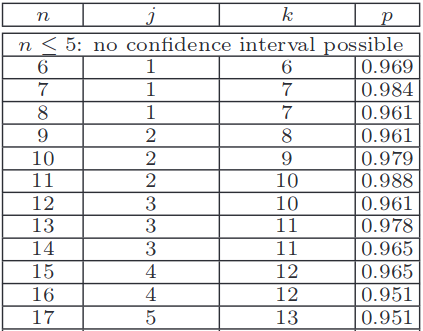
\includegraphics{illustrations/Table-CI-bis.png}
	}
	\caption{Table d'intervalles de confiance à $95\%$ \cite{leboudec2010performance}}\label{fig:tableCI}
\end{wrapfigure} 
Il est clair que {\textmu} est une valeur unique. Ce que nous cherchons est d'approcher {\textmu}. Pour ce faire, nous allons appliquer le théorème 2.1 relatif au calcul de l'intervalle de confiance de la médiane. Ce théorème permet de calculer l'intervalle de confiance de la médiane d'un ensemble de données. Comme $n = 10 $, nous avons besoin d'une table comme celle  donnée dans la Figure \ref{fig:tableCI}. A partir de la taille de l'ensemble ($n$) et le niveau de confiance $\gamma$, il est possible de trouver la borne inférieure de l'intervalle de confiance ($X_{(j)}$) et la borne supérieure de l'intervalle de confiance ($X_{(k)}$) à une probabilité $p$. Cette table fournit l'intervalle de confiance à $95 \%$ de confiance pour tout $n \leq 70$. A partir de $n \geq 71$, nous utilisons les deux formules de $ j $ (\ref{align:formule-j}) et $ k $ (\ref{align:formule-k}).

Dans notre exemple,  $n = 10$, ainsi, à une probabilité $95\%$, $j = 2$ et $ k = 9$, revenons aux données ordonnées,  $ X_{(2)} = 7.76 $ et  $ X_{(9)} =8.32 $. Autrement dit, à $95\%$, il est sûr que la valeur réelle de la médiane de l'ensemble de données, utilisées pour l'exemple, se trouve dans l'intervalle $[7.76, 8.32]$.


Prenons un exemple\footnote{Dans la table des intervalles de confiance, $p$ est le niveau de confiance, alors que ici, $p$ est la probabilité de succès.} où $n\geq 71$, soit p = 0.5 et $\eta$ = 1.96  pour  un intervalle de confiance à 95\%. Dans ce cas, 
$j \approx \lfloor 0.5n -  0.980\sqrt{n}\rfloor$ et $k\approx \lceil 0.5n + 0.980 \sqrt{n}\rceil + 1$.

Pour  $n = 100$ : $j = 40$ et $k = 61$, ainsi l'intervalle de confiance de la médiane est formé par $X_{(40)}$ et $X_{(61)}$.

Afin de montrer l'importance    de l'intervalle de confiance de la médiane dans l'élimination des valeurs aberrantes, nous donnons l'exemple suivant : 

\begin{table}[H]
	\centering
	\begin{tabular}{lccccc!{\color{red}\vrule}ccccc}
		\textbf{X}&	$ 7.68 $& $ 7.76 $& $ 7.76 $& $ 7.92 $& $ 8.08  $& $ 8.16 $& $ 8.24 $& $ 8.32 $& $ 8.72 $& $792$\\ \hline
		\textbf{Ordre}&	1&2&3&4&5&6&7&8&9&10\\
	\end{tabular}
	\caption{Exemple 2 d'application du théorème 2.1}
	\label{tab:outlierexample}
\end{table}

Le théorème $ 2.1 $ indique que l'intervalle de confiance de la médiane de l'ensemble de données dans la Table \ref{tab:outlierexample}  est formé par $ X_{(2)} $ et $X_{(9)}$, ce que donne $[7.76, 8.72]$ comme intervalle de confiance. L'intervalle de confiance obtenu pour cet ensemble de données est relativement différent de celui obtenu pour le premier ensemble de données. Toutefois, le deuxième intervalle de confiance est capable d'éliminer une valeur aberrante ($792$). 

\subsubsection{Méthode de score de  Wilson}
Les auteurs ont choisi le score de Wilson pour trouver l'intervalle de confiance de la médiane,  car il fonctionne bien, même avec un  nombre réduit d'échantillons \cite{doi:10.1002/sim.2164}. Le score De Wilson est calculé avec la formule \ref{align:wilson-formula}, avec  $n$ est la taille de l'ensemble de données, $p$ est la probabilité de succès et $z$ est égale à $1.96$ pour un niveau de confiance égale à $95\%$.
\begin{align}
w&= \frac{1}{1 + \frac{1}{n}z^2} \left( p + \frac{1}{2n} z^2 \pm z \sqrt{\frac{1}{n}p(1-p)+ \frac{1}{4n^2}z^2} \right)\label{align:wilson-formula}
\end{align} 
En pratique, le score de Wilson  produit deux valeurs appelées $w_l$ et $w_u$ dont leur valeurs sont dans $[0, 1]$. En multipliant $w_l$ et $w_u$ par $n$, nous obtenons les indices de le borne inférieure $l = nw_l$  et supérieure $u = nw_u$ de l'intervalle de confiance de la médiane. Nous précisons qu'en pratique, seule la partie entière de $l$ et $u$ qui indique l'indice. 
De la même manière que la méthode décrite dans la section \ref{CI-theorem}, nous ordonnons les $n$ données et nous construisons l'intervalle $[X_{(l)}, X_{(u)}]$.


En se basant uniquement sur l'ordre statistique, le score de Wilson produit des intervalles de confiance asymétriques dans le cas de distributions asymétriques, ce qui est le cas  des distributions des RTTs d'après l'étude \cite{DBLP:conf/infocom/FontugneMF15}. En outre, cette technique de calcul, basée uniquement sur l'ordre statistique de la variable permet d'éliminer les valeurs aberrantes indésirables.

Pour résumer, tout lien et pour chaque période, il est caractérisé par un ensemble de RTTs différentiels. Sur base de cet ensemble, les auteurs ont pu  caractériser ce lien par  la médiane  des RTTs différentiels.  De plus, en se basant encore sur cet ensemble, ils ont calculé l'intervalle de confiance de cette médiane. De la même manière, ils ont calculé une référence reprenant la médiane des RTTs différentiels et son intervalle de confiance. Cette référence prend en considération les observations des périodes précédentes.  



\subsection{Calcul de la référence} \label{reference-lissage}
L'état référence d'un lien représente le délai habituel d'un lien avec son intervalle de confiance habituel. Cette référence est utilisée pour détecter les délais anormaux. Précisément, cette référence est conservée  et  est mise à jour tout au long de l'analyse. C'est avec cette référence que l'état courant du lien est comparé. 
%Les auteurs ont proposé  l'approche  suivante, c'est comparer les deux intervalles de référence courant et référence. 

Présentons  brièvement  les séries chronologiques et leurs caractéristiques \cite{elementdestatistiques}.   
\begin{tcolorbox}[before upper={\parindent15pt}]
	Une \textit{série chronologique} est une série d'observations d'une variable réalisées à des dates successives notées $d_1$, $d_2$, ..., $d_n$. On distingue deux types de variables :
	
	\textit{variable  d'intensité} : les variables d'intensité, encore appelées \textbf{niveaux}, prennent leurs valeurs en des instants précis. Il en est de la température relevée dans un local tous les matins à $8$ heures, etc.
	
	\textit{variable de débit} : les variables de débit, encore appelées \textbf{flux}, concernent des intervalles de temps. C'est le cas, par exemple, de la quantité d'électricité consommée chaque jour par un ménage, etc.
	
	Si, dans le premier cas, les dates d'observation correspondent effectivement aux instants de mesure, le second cas, il est fréquent d'utiliser une notation unique; d'affecter la valeur observée pour une période déterminée au début de cette dernière, au centre ou à autre.
	
	L'étude d'une série chronologique concerne généralement trois objectifs : la description du phénomène étudié, son lissage et la détermination de prévisions.
\end{tcolorbox}

Dans notre cas, ce sont des périodes personnalisables, généralement une période d'une heure et les RTTs différentiels calculés durant, par exemple, une heure sont affectés au début de la période.

Etant donné que la médiane des RTTs différentiels est distribuée normalement,  la valeur prévue de la médiane est obtenue simplement en calculant la moyenne arithmétique des médianes observées précédemment, c'est qu'on appelle \textit{la moyenne mobile simple}. \textit{Cette manière d'agir ne se conçoit empiriquement que si le phénomène est stable\footnote{Prévision par moyenne mobile simple unilatérale (6.10.3)\cite{elementdestatistiques}.}}.
Etant donné que les anomalies peuvent altérer les valeurs moyennes et les rendre non pertinentes en tant que références, les auteurs ont utilisé    une prévision par lissage exponentiel 
plutôt qu'une prévision par moyenne mobile simple  en vue d'estimer la médiane des RTTs différentiels de référence tout en réduisant l'effet des anomalies sur cette médiane.
Si  la moyenne mobile simple  prend en compte les valeurs passées avec le même coefficient de pondération,  la prévision par lissage exponentiel peut supposer que plus une observation est ancienne, moins elle intervient dans la détermination de la prévision. 

Pour calculer la  valeur de la médiane des RTTs différentiels de référence $ \overline{m}_{t}$   courant la période $ t $ et pour le lien $l$, soit:

\begin{align}
\overline{m}_{t}& =  \alpha {m}_{t} + (1-  \alpha) \overline{m}_{t-1} \label{smoothe-formula}
\end{align} 

$m_t$ est la médiane des RTTs différentiels observée pour $l$ durant la période $t$. 

$ \overline{m}_{t-1}$  est la médiane des  RTTs différentiels  de référence durant la période $ t-1 $.  
$\alpha$ est un paramètre réel dans $[0,1]$, ce paramètre contrôle l'importance des nouvelles observations par rapport aux celles anciennes. Dans le cas de la présente étude, $\alpha$ est préféré d'être petit, précisément, $ \alpha = 0.01$.

Par ailleurs, l'utilisation de la formule \ref{smoothe-formula} pour la prévision de la médiane de référence nécessite de définir la valeur de la médiane initiale $ {m}_{1}$. Il existe plusieurs possibilités pour calculer $ {m}_{1}$, par exemple, il est possible de la définir comme étant la moyenne de deux, trois ou plusieurs premières observations. Dans leur implémentation, les auteurs ont choisi $\overline{m}_{1}$ comme étant la médiane de toutes les médianes des RTTs différentiels de $minSeen$  périodes, où $minSeen$ est un entier. Pour le reste des prévisions de la médiane de référence, on implique la médiane de référence précédente et  la médiane courante.

la référence d'un lien ne se limite pas seulement sur la médiane des RTTs différentiels mais en plus de la médiane,  on calcule  l'intervalle de confiance habituel de cette médiane. Les bornes de ce dernier sont calculées de la même manière que la médiane. Autrement dit, nous effectuons au fur et au mesure la prévision par lissage exponentiel de la borne inférieure de l'intervalle de confiance (respectivement borne supérieure). 

A ce stade, nous pouvons décrire un lien, durant une période donnée, par la médiane des RTTs différentiels et son intervalle de confiance. Ces même éléments illustre à la fois l'état courant du lien ainsi que son état référence. Sur base de ces état, on peut déclencher la détection des changements dans les délais de ce lien.

%Soient $d_i$, $d_j$, $d_k$, $d_l$, $d_m$ et $d_n$ des périodes quelconques  de l'analyse, et
Prenons un exemple où nous calculons la borne inférieure de l'intervalle de confiance de référence. 
Soient \textit{curCiLow} et \textit{refCiLow} la borne inférieure de l'intervalle de confiance de médiane courante et la borne inférieure de l'intervalle de confiance de la médiane référence.
Soit  $minSeen = 4$ le nombre d'observations assurant la représentativité de la référence. Soit $d_i$ la période courante de l'analyse et $d_1, d_2, ..., d_t$ les périodes de l'analyse. Nous distinguons trois cas :
\begin{itemize}
	\item  $d_i< d_{minSeen}$ : l'état référence est égal à l'état courant.
	\item  $d_i = d_{minSeen}$ : calcul de la référence pour la première fois en calculant la médiane de toutes les observations précédentes.
	\item  $d_i >d_{minSeen}$ : calcul de la référence en impliquant l'état courant et la référence précédente en appliquant l'équation \ref{smoothe-formula}.
\end{itemize}

Ces trois cas sont illustrés dans les  Tables \ref{result-3-cas}, ces derniers reprennent les résultats de l'analyse d'un nombre de traceroutes\footnote{\url{https://github.com/hayatbellafkih/SparkSalacaTraceroutesAnalysis/blob/master/rttDelaysSparkScala/src/main/resources/test/result_modified.json}, consultée  le $23/04/2019$. }.

\begin{table}[h]
	\captionsetup{justification= centering}
	
	\footnotesize{
		
		\caption{Exemple de calcul et mise à jour de la borne inférieure de l'intervalle  de confiance référence de la médiane }
		\label{result-3-cas}
		\begin{minipage}{.3\linewidth}
			
			\caption*{$d_i< d_{minSeen}$}
			\centering
			\begin{tabular}{|c|c|c|}
				\hline
				\textbf{$\mathbf{d_i}$} & \textbf{\textit{curCiLow}} &\textbf{\textit{refCiLow}} \\\hline
				$d_1$ &-3.197& -3.197\\\hline
				$d_2$ & -2.968&-2.968 \\\hline
				$d_3$ & -3.201& -3.201 \\\hline
			\end{tabular}
			
		\end{minipage}%
		\begin{minipage}{.3\linewidth}
			\caption*{ $d_i = d_{minSeen}$}
			\centering
			\begin{tabular}{|c|c|c|}
				\hline
				\textbf{$\mathbf{d_i}$} & \textbf{\textit{curCiLow}} &\textbf{\textit{refCiLow}} \\\hline
				$d_1$ &-3.197&-3.197\\\hline
				$d_2$ & -2.968&-3.197 \\\hline
				$d_3$ & -3.201& -3.197 \\\hline
				$d_4$ &-998.029& -3.197\\\hline
			\end{tabular}
		\end{minipage}%
		\begin{minipage}{.4\linewidth}
			\centering
			\caption*{$d_i >d_{minSeen}$}
			\begin{tabular}{|c|c|c|}
				\hline
				\textbf{$\mathbf{d_i}$} & \textbf{\textit{curCiLow}} &\textbf{\textit{refCiLow}} \\\hline
				$ d_1$ &-3.197&-3.197\\\hline
				$d_2$ & -2.968&-3.197 \\\hline
				$d_3$ & -3.201& -3.197 \\\hline
				$d_4$ &-998.029& -3.197\\\hline
				$d_5$ &-1098.029& -14.14532\\\hline
				$d_6$ &-3.029& -14.0341568\\\hline
			\end{tabular}
		\end{minipage} 
	}
	
\end{table}


\subsubsection{Détection des anomalies}
Afin d'identifier un changement dans le délai d'un lien, il suffit de comparer l'intervalle de confiance courant avec l'intervalle de 
confiance de référence. Cette comparaison ne se déclenche que si la référence de ce lien est assez représentable, autrement dit, le nombre d'observations est atteint pour calculer $\overline{m}_{1}$. Ce nombre est personnalisable et par défaut il est configuré sur $ 24 $. Si par exemple la durée d'une période est 1 heure, il faut avoir une journée d'observation pour construire la première référence du lien en question. Une fois la référence est  assez représentable, dorénavant,  elle est mise à jour en utilisant  le lissage exponentiel décrit dans la section \ref{reference-lissage}.
\begin{wrapfigure}{r}{.4\textwidth}
	\captionsetup{justification=centering}
	
	\resizebox{.4\textwidth}{!}{
		% Graphic for TeX using PGF
% Title: /home/hayat/RipeAtlasTraceroutesAnalysis/2019/Rapport/illustrations/explainCis
% Creator: Dia v0.97+git
% CreationDate: Tue Apr 30 10:45:36 2019
% For: hayat
% \usepackage{tikz}
% The following commands are not supported in PSTricks at present
% We define them conditionally, so when they are implemented,
% this pgf file will use them.
\ifx\du\undefined
  \newlength{\du}
\fi
\setlength{\du}{15\unitlength}
\begin{tikzpicture}[even odd rule]
\pgftransformxscale{1.000000}
\pgftransformyscale{-1.000000}
\definecolor{dialinecolor}{rgb}{0.000000, 0.000000, 0.000000}
\pgfsetstrokecolor{dialinecolor}
\pgfsetstrokeopacity{1.000000}
\definecolor{diafillcolor}{rgb}{1.000000, 1.000000, 1.000000}
\pgfsetfillcolor{diafillcolor}
\pgfsetfillopacity{1.000000}
\pgfsetlinewidth{0.100000\du}
\pgfsetdash{}{0pt}
\pgfsetbuttcap
{
\definecolor{diafillcolor}{rgb}{0.000000, 0.000000, 0.000000}
\pgfsetfillcolor{diafillcolor}
\pgfsetfillopacity{1.000000}
% was here!!!
}
\definecolor{dialinecolor}{rgb}{0.000000, 0.000000, 0.000000}
\pgfsetstrokecolor{dialinecolor}
\pgfsetstrokeopacity{1.000000}
\draw (11.337256\du,5.581598\du)--(11.354934\du,10.884899\du);
\pgfsetlinewidth{0.100000\du}
\pgfsetdash{}{0pt}
\pgfsetmiterjoin
\pgfsetbuttcap
\definecolor{diafillcolor}{rgb}{0.000000, 0.000000, 0.000000}
\pgfsetfillcolor{diafillcolor}
\pgfsetfillopacity{1.000000}
\definecolor{dialinecolor}{rgb}{0.000000, 0.000000, 0.000000}
\pgfsetstrokecolor{dialinecolor}
\pgfsetstrokeopacity{1.000000}
\pgfpathmoveto{\pgfpoint{11.337256\du}{5.581598\du}}
\pgfpathcurveto{\pgfpoint{11.462256\du}{5.581181\du}}{\pgfpoint{11.587671\du}{5.705764\du}}{\pgfpoint{11.588088\du}{5.830763\du}}
\pgfpathcurveto{\pgfpoint{11.588505\du}{5.955763\du}}{\pgfpoint{11.463922\du}{6.081179\du}}{\pgfpoint{11.338923\du}{6.081595\du}}
\pgfpathcurveto{\pgfpoint{11.213924\du}{6.082012\du}}{\pgfpoint{11.088508\du}{5.957429\du}}{\pgfpoint{11.088091\du}{5.832430\du}}
\pgfpathcurveto{\pgfpoint{11.087674\du}{5.707431\du}}{\pgfpoint{11.212257\du}{5.582015\du}}{\pgfpoint{11.337256\du}{5.581598\du}}
\pgfpathclose
\pgfusepath{fill,stroke}
\pgfsetlinewidth{0.100000\du}
\pgfsetdash{}{0pt}
\pgfsetmiterjoin
\pgfsetbuttcap
\definecolor{diafillcolor}{rgb}{0.000000, 0.000000, 0.000000}
\pgfsetfillcolor{diafillcolor}
\pgfsetfillopacity{1.000000}
\definecolor{dialinecolor}{rgb}{0.000000, 0.000000, 0.000000}
\pgfsetstrokecolor{dialinecolor}
\pgfsetstrokeopacity{1.000000}
\pgfpathmoveto{\pgfpoint{11.354934\du}{10.884899\du}}
\pgfpathcurveto{\pgfpoint{11.229935\du}{10.885316\du}}{\pgfpoint{11.104519\du}{10.760733\du}}{\pgfpoint{11.104102\du}{10.635734\du}}
\pgfpathcurveto{\pgfpoint{11.103685\du}{10.510734\du}}{\pgfpoint{11.228268\du}{10.385318\du}}{\pgfpoint{11.353267\du}{10.384902\du}}
\pgfpathcurveto{\pgfpoint{11.478267\du}{10.384485\du}}{\pgfpoint{11.603683\du}{10.509068\du}}{\pgfpoint{11.604099\du}{10.634067\du}}
\pgfpathcurveto{\pgfpoint{11.604516\du}{10.759066\du}}{\pgfpoint{11.479933\du}{10.884482\du}}{\pgfpoint{11.354934\du}{10.884899\du}}
\pgfpathclose
\pgfusepath{fill,stroke}
% setfont left to latex
\definecolor{dialinecolor}{rgb}{0.000000, 0.000000, 0.000000}
\pgfsetstrokecolor{dialinecolor}
\pgfsetstrokeopacity{1.000000}
\definecolor{diafillcolor}{rgb}{0.000000, 0.000000, 0.000000}
\pgfsetfillcolor{diafillcolor}
\pgfsetfillopacity{1.000000}
\node[anchor=base west,inner sep=0pt,outer sep=0pt,color=dialinecolor] at (11.100944\du,8.615472\du){-};
\pgfsetlinewidth{0.100000\du}
\pgfsetdash{}{0pt}
\pgfsetbuttcap
{
\definecolor{diafillcolor}{rgb}{0.000000, 0.000000, 0.000000}
\pgfsetfillcolor{diafillcolor}
\pgfsetfillopacity{1.000000}
% was here!!!
}
\definecolor{dialinecolor}{rgb}{0.000000, 0.000000, 0.000000}
\pgfsetstrokecolor{dialinecolor}
\pgfsetstrokeopacity{1.000000}
\draw (13.281660\du,6.080057\du)--(13.276752\du,10.374707\du);
\pgfsetlinewidth{0.100000\du}
\pgfsetdash{}{0pt}
\pgfsetmiterjoin
\pgfsetbuttcap
\definecolor{diafillcolor}{rgb}{1.000000, 1.000000, 1.000000}
\pgfsetfillcolor{diafillcolor}
\pgfsetfillopacity{1.000000}
\definecolor{dialinecolor}{rgb}{0.000000, 0.000000, 0.000000}
\pgfsetstrokecolor{dialinecolor}
\pgfsetstrokeopacity{1.000000}
\pgfpathmoveto{\pgfpoint{13.282231\du}{5.580057\du}}
\pgfpathcurveto{\pgfpoint{13.407231\du}{5.580200\du}}{\pgfpoint{13.532088\du}{5.705343\du}}{\pgfpoint{13.531945\du}{5.830343\du}}
\pgfpathcurveto{\pgfpoint{13.531802\du}{5.955343\du}}{\pgfpoint{13.406660\du}{6.080200\du}}{\pgfpoint{13.281660\du}{6.080057\du}}
\pgfpathcurveto{\pgfpoint{13.156660\du}{6.079914\du}}{\pgfpoint{13.031803\du}{5.954771\du}}{\pgfpoint{13.031946\du}{5.829771\du}}
\pgfpathcurveto{\pgfpoint{13.032088\du}{5.704771\du}}{\pgfpoint{13.157231\du}{5.579914\du}}{\pgfpoint{13.282231\du}{5.580057\du}}
\pgfpathclose
\pgfusepath{fill,stroke}
\pgfsetlinewidth{0.100000\du}
\pgfsetdash{}{0pt}
\pgfsetmiterjoin
\pgfsetbuttcap
\definecolor{diafillcolor}{rgb}{1.000000, 1.000000, 1.000000}
\pgfsetfillcolor{diafillcolor}
\pgfsetfillopacity{1.000000}
\definecolor{dialinecolor}{rgb}{0.000000, 0.000000, 0.000000}
\pgfsetstrokecolor{dialinecolor}
\pgfsetstrokeopacity{1.000000}
\pgfpathmoveto{\pgfpoint{13.276180\du}{10.874707\du}}
\pgfpathcurveto{\pgfpoint{13.151180\du}{10.874564\du}}{\pgfpoint{13.026323\du}{10.749421\du}}{\pgfpoint{13.026466\du}{10.624421\du}}
\pgfpathcurveto{\pgfpoint{13.026609\du}{10.499421\du}}{\pgfpoint{13.151752\du}{10.374564\du}}{\pgfpoint{13.276752\du}{10.374707\du}}
\pgfpathcurveto{\pgfpoint{13.401751\du}{10.374850\du}}{\pgfpoint{13.526609\du}{10.499993\du}}{\pgfpoint{13.526466\du}{10.624993\du}}
\pgfpathcurveto{\pgfpoint{13.526323\du}{10.749993\du}}{\pgfpoint{13.401180\du}{10.874850\du}}{\pgfpoint{13.276180\du}{10.874707\du}}
\pgfpathclose
\pgfusepath{fill,stroke}
% setfont left to latex
\definecolor{dialinecolor}{rgb}{0.000000, 0.000000, 0.000000}
\pgfsetstrokecolor{dialinecolor}
\pgfsetstrokeopacity{1.000000}
\definecolor{diafillcolor}{rgb}{0.000000, 0.000000, 0.000000}
\pgfsetfillcolor{diafillcolor}
\pgfsetfillopacity{1.000000}
\node[anchor=base west,inner sep=0pt,outer sep=0pt,color=dialinecolor] at (13.012306\du,8.716238\du){*};
% setfont left to latex
\definecolor{dialinecolor}{rgb}{0.000000, 0.000000, 0.000000}
\pgfsetstrokecolor{dialinecolor}
\pgfsetstrokeopacity{1.000000}
\definecolor{diafillcolor}{rgb}{0.000000, 0.000000, 0.000000}
\pgfsetfillcolor{diafillcolor}
\pgfsetfillopacity{1.000000}
\node[anchor=base west,inner sep=0pt,outer sep=0pt,color=dialinecolor] at (14.943501\du,6.005862\du){referenceCiLow};
% setfont left to latex
\definecolor{dialinecolor}{rgb}{0.000000, 0.000000, 0.000000}
\pgfsetstrokecolor{dialinecolor}
\pgfsetstrokeopacity{1.000000}
\definecolor{diafillcolor}{rgb}{0.000000, 0.000000, 0.000000}
\pgfsetfillcolor{diafillcolor}
\pgfsetfillopacity{1.000000}
\node[anchor=base west,inner sep=0pt,outer sep=0pt,color=dialinecolor] at (14.977088\du,10.910678\du){referenceCiHight};
\pgfsetlinewidth{0.100000\du}
\pgfsetdash{}{0pt}
\pgfsetbuttcap
{
\definecolor{diafillcolor}{rgb}{0.000000, 0.000000, 0.000000}
\pgfsetfillcolor{diafillcolor}
\pgfsetfillopacity{1.000000}
% was here!!!
\pgfsetarrowsend{to}
\definecolor{dialinecolor}{rgb}{0.000000, 0.000000, 0.000000}
\pgfsetstrokecolor{dialinecolor}
\pgfsetstrokeopacity{1.000000}
\draw (14.749046\du,5.776052\du)--(13.723742\du,5.776052\du);
}
\pgfsetlinewidth{0.100000\du}
\pgfsetdash{}{0pt}
\pgfsetbuttcap
{
\definecolor{diafillcolor}{rgb}{0.000000, 0.000000, 0.000000}
\pgfsetfillcolor{diafillcolor}
\pgfsetfillopacity{1.000000}
% was here!!!
\pgfsetarrowsend{to}
\definecolor{dialinecolor}{rgb}{0.000000, 0.000000, 0.000000}
\pgfsetstrokecolor{dialinecolor}
\pgfsetstrokeopacity{1.000000}
\draw (14.885667\du,10.752646\du)--(13.860362\du,10.752646\du);
}
% setfont left to latex
\definecolor{dialinecolor}{rgb}{0.000000, 0.000000, 0.000000}
\pgfsetstrokecolor{dialinecolor}
\pgfsetstrokeopacity{1.000000}
\definecolor{diafillcolor}{rgb}{0.000000, 0.000000, 0.000000}
\pgfsetfillcolor{diafillcolor}
\pgfsetfillopacity{1.000000}
\node[anchor=base west,inner sep=0pt,outer sep=0pt,color=dialinecolor] at (14.959411\du,8.365094\du){referenceMedian};
\pgfsetlinewidth{0.100000\du}
\pgfsetdash{}{0pt}
\pgfsetbuttcap
{
\definecolor{diafillcolor}{rgb}{0.000000, 0.000000, 0.000000}
\pgfsetfillcolor{diafillcolor}
\pgfsetfillopacity{1.000000}
% was here!!!
\pgfsetarrowsend{to}
\definecolor{dialinecolor}{rgb}{0.000000, 0.000000, 0.000000}
\pgfsetstrokecolor{dialinecolor}
\pgfsetstrokeopacity{1.000000}
\draw (14.832634\du,8.189384\du)--(13.807329\du,8.189384\du);
}
% setfont left to latex
\definecolor{dialinecolor}{rgb}{0.000000, 0.000000, 0.000000}
\pgfsetstrokecolor{dialinecolor}
\pgfsetstrokeopacity{1.000000}
\definecolor{diafillcolor}{rgb}{0.000000, 0.000000, 0.000000}
\pgfsetfillcolor{diafillcolor}
\pgfsetfillopacity{1.000000}
\node[anchor=base west,inner sep=0pt,outer sep=0pt,color=dialinecolor] at (4.968494\du,6.031641\du){currentCiLow};
% setfont left to latex
\definecolor{dialinecolor}{rgb}{0.000000, 0.000000, 0.000000}
\pgfsetstrokecolor{dialinecolor}
\pgfsetstrokeopacity{1.000000}
\definecolor{diafillcolor}{rgb}{0.000000, 0.000000, 0.000000}
\pgfsetfillcolor{diafillcolor}
\pgfsetfillopacity{1.000000}
\node[anchor=base west,inner sep=0pt,outer sep=0pt,color=dialinecolor] at (4.913694\du,10.706647\du){currentCiHight};
\pgfsetlinewidth{0.100000\du}
\pgfsetdash{}{0pt}
\pgfsetbuttcap
{
\definecolor{diafillcolor}{rgb}{0.000000, 0.000000, 0.000000}
\pgfsetfillcolor{diafillcolor}
\pgfsetfillopacity{1.000000}
% was here!!!
\pgfsetarrowsstart{to}
\definecolor{dialinecolor}{rgb}{0.000000, 0.000000, 0.000000}
\pgfsetstrokecolor{dialinecolor}
\pgfsetstrokeopacity{1.000000}
\draw (10.797325\du,10.637003\du)--(9.772020\du,10.637003\du);
}
% setfont left to latex
\definecolor{dialinecolor}{rgb}{0.000000, 0.000000, 0.000000}
\pgfsetstrokecolor{dialinecolor}
\pgfsetstrokeopacity{1.000000}
\definecolor{diafillcolor}{rgb}{0.000000, 0.000000, 0.000000}
\pgfsetfillcolor{diafillcolor}
\pgfsetfillopacity{1.000000}
\node[anchor=base west,inner sep=0pt,outer sep=0pt,color=dialinecolor] at (5.037437\du,8.355517\du){currentMedian};
\pgfsetlinewidth{0.100000\du}
\pgfsetdash{}{0pt}
\pgfsetbuttcap
{
\definecolor{diafillcolor}{rgb}{0.000000, 0.000000, 0.000000}
\pgfsetfillcolor{diafillcolor}
\pgfsetfillopacity{1.000000}
% was here!!!
\pgfsetarrowsstart{to}
\definecolor{dialinecolor}{rgb}{0.000000, 0.000000, 0.000000}
\pgfsetstrokecolor{dialinecolor}
\pgfsetstrokeopacity{1.000000}
\draw (10.961224\du,8.207061\du)--(9.935920\du,8.207061\du);
}
\pgfsetlinewidth{0.100000\du}
\pgfsetdash{}{0pt}
\pgfsetbuttcap
{
\definecolor{diafillcolor}{rgb}{0.000000, 0.000000, 0.000000}
\pgfsetfillcolor{diafillcolor}
\pgfsetfillopacity{1.000000}
% was here!!!
\pgfsetarrowsstart{to}
\definecolor{dialinecolor}{rgb}{0.000000, 0.000000, 0.000000}
\pgfsetstrokecolor{dialinecolor}
\pgfsetstrokeopacity{1.000000}
\draw (10.977134\du,5.887751\du)--(9.951829\du,5.887751\du);
}
\end{tikzpicture}

	}
	\caption{Nomination utilisée}
	\label{fig:explainCis}
\end{wrapfigure}


Soit \textit{currentCiLow}, \textit{currentCiHight}, \textit{currentMedian}, \textit{referenceCiLow}, \textit{referenceCiHight}, \textit{referenceMedian} dénote respectivement la borne inférieure de l'intervalle de confiance de médiane courante, la borne supérieure de l'intervalle de confiance de la médiane courante, la médiane des RTTs différentiels courante, la borne inférieure de l'intervalle de confiance de la médiane de référence, la borne supérieure de l'intervalle de confiance de la médiane de référence, la médiane des RTTs différentiels de référence. La Figure 	\ref{fig:explainCis} illustre la nomination utilisée dans la Figure \ref{fig:anomalies}.

Dans le travail de référence, une anomalie est détectée si les conditions \ref{align:condition-1} et \ref{align:condition-2} sont vraies. La première condition évalue le chevauchement entre les deux intervalles de confiance. Or, la deuxième condition assure que seulement la  différence entre la médiane des RTTs différentiels courante et celle de référence dépassant $1 ms$ qui est prise en compte.
\begin{align}
(currentCiLow > referenceCiHight OU  currentCiHight <  referenceCiLow) \label{align:condition-1}
\end{align}
\begin{align}
(abs(currentMedian -- referenceMedian) > 1 ) \label{align:condition-2}
\end{align}
%Nous illustrons la comparaison des intervalles de confiance dans la Figure \ref{fig:anomalies}.
La Figure \ref{fig:anomalies} illustre les différents cas possibles de positionnement des deux intervalles de confiance. Nous précisons que,  dans les Figures	\ref{fig:explainCis} et \ref{fig:anomalies},  la longueur des intervalles de confiance ainsi que le positionnement de la médiane n'est pas exacte, ils sont donnés pour l'illustration de la comparaison. Nous supposons que la condition \ref{align:condition-2} est vraie et les différents cas possibles sont donnés dans la Figure 	\ref{fig:anomalies}.

\begin{figure}[H]
	\centering
	\captionsetup{justification=centering}
	\resizebox{\textwidth}{!}{
		% Graphic for TeX using PGF
% Title: /home/hayat/RipeAtlasTraceroutesAnalysis/2019/Rapport/illustrations/casesAnomalies.dia
% Creator: Dia v0.97+git
% CreationDate: Tue Apr 30 01:04:07 2019
% For: hayat
% \usepackage{tikz}
% The following commands are not supported in PSTricks at present
% We define them conditionally, so when they are implemented,
% this pgf file will use them.
\ifx\du\undefined
  \newlength{\du}
\fi
\setlength{\du}{15\unitlength}
\begin{tikzpicture}[even odd rule]
\pgftransformxscale{1.000000}
\pgftransformyscale{-1.000000}
\definecolor{dialinecolor}{rgb}{0.000000, 0.000000, 0.000000}
\pgfsetstrokecolor{dialinecolor}
\pgfsetstrokeopacity{1.000000}
\definecolor{diafillcolor}{rgb}{1.000000, 1.000000, 1.000000}
\pgfsetfillcolor{diafillcolor}
\pgfsetfillopacity{1.000000}
\pgfsetlinewidth{0.100000\du}
\pgfsetdash{}{0pt}
\pgfsetbuttcap
{
\definecolor{diafillcolor}{rgb}{0.000000, 0.000000, 0.000000}
\pgfsetfillcolor{diafillcolor}
\pgfsetfillopacity{1.000000}
% was here!!!
\pgfsetarrowsend{stealth}
\definecolor{dialinecolor}{rgb}{0.000000, 0.000000, 0.000000}
\pgfsetstrokecolor{dialinecolor}
\pgfsetstrokeopacity{1.000000}
\draw (5.463816\du,9.994870\du)--(56.365537\du,10.059352\du);
}
\pgfsetlinewidth{0.100000\du}
\pgfsetdash{}{0pt}
\pgfsetbuttcap
{
\definecolor{diafillcolor}{rgb}{0.000000, 0.000000, 0.000000}
\pgfsetfillcolor{diafillcolor}
\pgfsetfillopacity{1.000000}
% was here!!!
\pgfsetarrowsend{stealth}
\definecolor{dialinecolor}{rgb}{0.000000, 0.000000, 0.000000}
\pgfsetstrokecolor{dialinecolor}
\pgfsetstrokeopacity{1.000000}
\draw (8.950025\du,10.850000\du)--(8.977679\du,-3.524568\du);
}
\pgfsetlinewidth{0.100000\du}
\pgfsetdash{}{0pt}
\pgfsetbuttcap
{
\definecolor{diafillcolor}{rgb}{0.000000, 0.000000, 0.000000}
\pgfsetfillcolor{diafillcolor}
\pgfsetfillopacity{1.000000}
% was here!!!
}
\definecolor{dialinecolor}{rgb}{0.000000, 0.000000, 0.000000}
\pgfsetstrokecolor{dialinecolor}
\pgfsetstrokeopacity{1.000000}
\draw (17.091618\du,5.650000\du)--(17.091726\du,9.300000\du);
\pgfsetlinewidth{0.100000\du}
\pgfsetdash{}{0pt}
\pgfsetmiterjoin
\pgfsetbuttcap
\definecolor{diafillcolor}{rgb}{0.000000, 0.000000, 0.000000}
\pgfsetfillcolor{diafillcolor}
\pgfsetfillopacity{1.000000}
\definecolor{dialinecolor}{rgb}{0.000000, 0.000000, 0.000000}
\pgfsetstrokecolor{dialinecolor}
\pgfsetstrokeopacity{1.000000}
\pgfpathmoveto{\pgfpoint{17.091618\du}{5.650000\du}}
\pgfpathcurveto{\pgfpoint{17.216618\du}{5.649996\du}}{\pgfpoint{17.341622\du}{5.774993\du}}{\pgfpoint{17.341625\du}{5.899993\du}}
\pgfpathcurveto{\pgfpoint{17.341629\du}{6.024993\du}}{\pgfpoint{17.216633\du}{6.149996\du}}{\pgfpoint{17.091633\du}{6.150000\du}}
\pgfpathcurveto{\pgfpoint{16.966633\du}{6.150004\du}}{\pgfpoint{16.841629\du}{6.025007\du}}{\pgfpoint{16.841625\du}{5.900007\du}}
\pgfpathcurveto{\pgfpoint{16.841622\du}{5.775007\du}}{\pgfpoint{16.966618\du}{5.650004\du}}{\pgfpoint{17.091618\du}{5.650000\du}}
\pgfpathclose
\pgfusepath{fill,stroke}
\pgfsetlinewidth{0.100000\du}
\pgfsetdash{}{0pt}
\pgfsetmiterjoin
\pgfsetbuttcap
\definecolor{diafillcolor}{rgb}{0.000000, 0.000000, 0.000000}
\pgfsetfillcolor{diafillcolor}
\pgfsetfillopacity{1.000000}
\definecolor{dialinecolor}{rgb}{0.000000, 0.000000, 0.000000}
\pgfsetstrokecolor{dialinecolor}
\pgfsetstrokeopacity{1.000000}
\pgfpathmoveto{\pgfpoint{17.091726\du}{9.300000\du}}
\pgfpathcurveto{\pgfpoint{16.966726\du}{9.300004\du}}{\pgfpoint{16.841723\du}{9.175007\du}}{\pgfpoint{16.841719\du}{9.050007\du}}
\pgfpathcurveto{\pgfpoint{16.841715\du}{8.925007\du}}{\pgfpoint{16.966712\du}{8.800004\du}}{\pgfpoint{17.091712\du}{8.800000\du}}
\pgfpathcurveto{\pgfpoint{17.216712\du}{8.799996\du}}{\pgfpoint{17.341715\du}{8.924993\du}}{\pgfpoint{17.341719\du}{9.049993\du}}
\pgfpathcurveto{\pgfpoint{17.341723\du}{9.174993\du}}{\pgfpoint{17.216726\du}{9.299996\du}}{\pgfpoint{17.091726\du}{9.300000\du}}
\pgfpathclose
\pgfusepath{fill,stroke}
\pgfsetlinewidth{0.100000\du}
\pgfsetdash{}{0pt}
\pgfsetbuttcap
{
\definecolor{diafillcolor}{rgb}{0.000000, 0.000000, 0.000000}
\pgfsetfillcolor{diafillcolor}
\pgfsetfillopacity{1.000000}
% was here!!!
}
\definecolor{dialinecolor}{rgb}{0.000000, 0.000000, 0.000000}
\pgfsetstrokecolor{dialinecolor}
\pgfsetstrokeopacity{1.000000}
\draw (19.099686\du,0.525845\du)--(19.094778\du,4.820495\du);
\pgfsetlinewidth{0.100000\du}
\pgfsetdash{}{0pt}
\pgfsetmiterjoin
\pgfsetbuttcap
\definecolor{diafillcolor}{rgb}{1.000000, 1.000000, 1.000000}
\pgfsetfillcolor{diafillcolor}
\pgfsetfillopacity{1.000000}
\definecolor{dialinecolor}{rgb}{0.000000, 0.000000, 0.000000}
\pgfsetstrokecolor{dialinecolor}
\pgfsetstrokeopacity{1.000000}
\pgfpathmoveto{\pgfpoint{19.100257\du}{0.025845\du}}
\pgfpathcurveto{\pgfpoint{19.225257\du}{0.025988\du}}{\pgfpoint{19.350114\du}{0.151131\du}}{\pgfpoint{19.349971\du}{0.276131\du}}
\pgfpathcurveto{\pgfpoint{19.349828\du}{0.401131\du}}{\pgfpoint{19.224686\du}{0.525988\du}}{\pgfpoint{19.099686\du}{0.525845\du}}
\pgfpathcurveto{\pgfpoint{18.974686\du}{0.525702\du}}{\pgfpoint{18.849829\du}{0.400559\du}}{\pgfpoint{18.849972\du}{0.275559\du}}
\pgfpathcurveto{\pgfpoint{18.850114\du}{0.150559\du}}{\pgfpoint{18.975257\du}{0.025702\du}}{\pgfpoint{19.100257\du}{0.025845\du}}
\pgfpathclose
\pgfusepath{fill,stroke}
\pgfsetlinewidth{0.100000\du}
\pgfsetdash{}{0pt}
\pgfsetmiterjoin
\pgfsetbuttcap
\definecolor{diafillcolor}{rgb}{1.000000, 1.000000, 1.000000}
\pgfsetfillcolor{diafillcolor}
\pgfsetfillopacity{1.000000}
\definecolor{dialinecolor}{rgb}{0.000000, 0.000000, 0.000000}
\pgfsetstrokecolor{dialinecolor}
\pgfsetstrokeopacity{1.000000}
\pgfpathmoveto{\pgfpoint{19.094206\du}{5.320495\du}}
\pgfpathcurveto{\pgfpoint{18.969206\du}{5.320352\du}}{\pgfpoint{18.844349\du}{5.195209\du}}{\pgfpoint{18.844492\du}{5.070209\du}}
\pgfpathcurveto{\pgfpoint{18.844635\du}{4.945210\du}}{\pgfpoint{18.969778\du}{4.820352\du}}{\pgfpoint{19.094778\du}{4.820495\du}}
\pgfpathcurveto{\pgfpoint{19.219777\du}{4.820638\du}}{\pgfpoint{19.344635\du}{4.945781\du}}{\pgfpoint{19.344492\du}{5.070781\du}}
\pgfpathcurveto{\pgfpoint{19.344349\du}{5.195781\du}}{\pgfpoint{19.219206\du}{5.320638\du}}{\pgfpoint{19.094206\du}{5.320495\du}}
\pgfpathclose
\pgfusepath{fill,stroke}
\pgfsetdash{}{0pt}
\pgfsetmiterjoin
% setfont left to latex
\pgfsetlinewidth{0.050000\du}
\pgfsetlinewidth{0.100000\du}
\definecolor{dialinecolor}{rgb}{0.000000, 0.000000, 0.000000}
\pgfsetstrokecolor{dialinecolor}
\pgfsetstrokeopacity{1.000000}
\draw (14.988620\du,10.050000\du)--(14.988620\du,12.400000\du);
\definecolor{dialinecolor}{rgb}{1.000000, 1.000000, 1.000000}
\pgfsetstrokecolor{dialinecolor}
\pgfsetstrokeopacity{1.000000}
\definecolor{diafillcolor}{rgb}{1.000000, 1.000000, 1.000000}
\pgfsetfillcolor{diafillcolor}
\pgfsetfillopacity{1.000000}
\node[anchor=base,inner sep=0pt, outer sep=0pt,color=dialinecolor] at (14.988620\du,13.150000\du){0};
\definecolor{dialinecolor}{rgb}{0.000000, 0.000000, 0.000000}
\pgfsetstrokecolor{dialinecolor}
\pgfsetstrokeopacity{1.000000}
\draw (21.189262\du,10.050000\du)--(21.189262\du,12.400000\du);
\definecolor{dialinecolor}{rgb}{1.000000, 1.000000, 1.000000}
\pgfsetstrokecolor{dialinecolor}
\pgfsetstrokeopacity{1.000000}
\definecolor{diafillcolor}{rgb}{1.000000, 1.000000, 1.000000}
\pgfsetfillcolor{diafillcolor}
\pgfsetfillopacity{1.000000}
\node[anchor=base,inner sep=0pt, outer sep=0pt,color=dialinecolor] at (21.189262\du,13.150000\du){1};
\definecolor{dialinecolor}{rgb}{0.000000, 0.000000, 0.000000}
\pgfsetstrokecolor{dialinecolor}
\pgfsetstrokeopacity{1.000000}
\draw (27.389904\du,10.050000\du)--(27.389904\du,12.400000\du);
\definecolor{dialinecolor}{rgb}{1.000000, 1.000000, 1.000000}
\pgfsetstrokecolor{dialinecolor}
\pgfsetstrokeopacity{1.000000}
\definecolor{diafillcolor}{rgb}{1.000000, 1.000000, 1.000000}
\pgfsetfillcolor{diafillcolor}
\pgfsetfillopacity{1.000000}
\node[anchor=base,inner sep=0pt, outer sep=0pt,color=dialinecolor] at (27.389904\du,13.150000\du){2};
\definecolor{dialinecolor}{rgb}{0.000000, 0.000000, 0.000000}
\pgfsetstrokecolor{dialinecolor}
\pgfsetstrokeopacity{1.000000}
\draw (33.590545\du,10.050000\du)--(33.590545\du,12.400000\du);
\definecolor{dialinecolor}{rgb}{1.000000, 1.000000, 1.000000}
\pgfsetstrokecolor{dialinecolor}
\pgfsetstrokeopacity{1.000000}
\definecolor{diafillcolor}{rgb}{1.000000, 1.000000, 1.000000}
\pgfsetfillcolor{diafillcolor}
\pgfsetfillopacity{1.000000}
\node[anchor=base,inner sep=0pt, outer sep=0pt,color=dialinecolor] at (33.590545\du,13.150000\du){3};
\definecolor{dialinecolor}{rgb}{0.000000, 0.000000, 0.000000}
\pgfsetstrokecolor{dialinecolor}
\pgfsetstrokeopacity{1.000000}
\draw (39.791187\du,10.050000\du)--(39.791187\du,12.400000\du);
\definecolor{dialinecolor}{rgb}{1.000000, 1.000000, 1.000000}
\pgfsetstrokecolor{dialinecolor}
\pgfsetstrokeopacity{1.000000}
\definecolor{diafillcolor}{rgb}{1.000000, 1.000000, 1.000000}
\pgfsetfillcolor{diafillcolor}
\pgfsetfillopacity{1.000000}
\node[anchor=base,inner sep=0pt, outer sep=0pt,color=dialinecolor] at (39.791187\du,13.150000\du){4};
\definecolor{dialinecolor}{rgb}{0.000000, 0.000000, 0.000000}
\pgfsetstrokecolor{dialinecolor}
\pgfsetstrokeopacity{1.000000}
\draw (45.991829\du,10.050000\du)--(45.991829\du,12.400000\du);
\definecolor{dialinecolor}{rgb}{1.000000, 1.000000, 1.000000}
\pgfsetstrokecolor{dialinecolor}
\pgfsetstrokeopacity{1.000000}
\definecolor{diafillcolor}{rgb}{1.000000, 1.000000, 1.000000}
\pgfsetfillcolor{diafillcolor}
\pgfsetfillopacity{1.000000}
\node[anchor=base,inner sep=0pt, outer sep=0pt,color=dialinecolor] at (45.991829\du,13.150000\du){5};
\definecolor{dialinecolor}{rgb}{0.000000, 0.000000, 0.000000}
\pgfsetstrokecolor{dialinecolor}
\pgfsetstrokeopacity{1.000000}
\draw (14.988620\du,10.050000\du)--(52.192470\du,10.050000\du);
\pgfsetlinewidth{0.100000\du}
\pgfsetdash{}{0pt}
\pgfsetbuttcap
{
\definecolor{diafillcolor}{rgb}{0.000000, 0.000000, 0.000000}
\pgfsetfillcolor{diafillcolor}
\pgfsetfillopacity{1.000000}
% was here!!!
}
\definecolor{dialinecolor}{rgb}{0.000000, 0.000000, 0.000000}
\pgfsetstrokecolor{dialinecolor}
\pgfsetstrokeopacity{1.000000}
\draw (23.107321\du,-0.509539\du)--(23.107430\du,3.140461\du);
\pgfsetlinewidth{0.100000\du}
\pgfsetdash{}{0pt}
\pgfsetmiterjoin
\pgfsetbuttcap
\definecolor{diafillcolor}{rgb}{0.000000, 0.000000, 0.000000}
\pgfsetfillcolor{diafillcolor}
\pgfsetfillopacity{1.000000}
\definecolor{dialinecolor}{rgb}{0.000000, 0.000000, 0.000000}
\pgfsetstrokecolor{dialinecolor}
\pgfsetstrokeopacity{1.000000}
\pgfpathmoveto{\pgfpoint{23.107321\du}{-0.509539\du}}
\pgfpathcurveto{\pgfpoint{23.232321\du}{-0.509543\du}}{\pgfpoint{23.357325\du}{-0.384547\du}}{\pgfpoint{23.357328\du}{-0.259547\du}}
\pgfpathcurveto{\pgfpoint{23.357332\du}{-0.134547\du}}{\pgfpoint{23.232336\du}{-0.009543\du}}{\pgfpoint{23.107336\du}{-0.009539\du}}
\pgfpathcurveto{\pgfpoint{22.982336\du}{-0.009535\du}}{\pgfpoint{22.857332\du}{-0.134532\du}}{\pgfpoint{22.857328\du}{-0.259532\du}}
\pgfpathcurveto{\pgfpoint{22.857325\du}{-0.384532\du}}{\pgfpoint{22.982321\du}{-0.509535\du}}{\pgfpoint{23.107321\du}{-0.509539\du}}
\pgfpathclose
\pgfusepath{fill,stroke}
\pgfsetlinewidth{0.100000\du}
\pgfsetdash{}{0pt}
\pgfsetmiterjoin
\pgfsetbuttcap
\definecolor{diafillcolor}{rgb}{0.000000, 0.000000, 0.000000}
\pgfsetfillcolor{diafillcolor}
\pgfsetfillopacity{1.000000}
\definecolor{dialinecolor}{rgb}{0.000000, 0.000000, 0.000000}
\pgfsetstrokecolor{dialinecolor}
\pgfsetstrokeopacity{1.000000}
\pgfpathmoveto{\pgfpoint{23.107430\du}{3.140461\du}}
\pgfpathcurveto{\pgfpoint{22.982430\du}{3.140465\du}}{\pgfpoint{22.857426\du}{3.015468\du}}{\pgfpoint{22.857422\du}{2.890468\du}}
\pgfpathcurveto{\pgfpoint{22.857418\du}{2.765468\du}}{\pgfpoint{22.982415\du}{2.640465\du}}{\pgfpoint{23.107415\du}{2.640461\du}}
\pgfpathcurveto{\pgfpoint{23.232415\du}{2.640457\du}}{\pgfpoint{23.357418\du}{2.765453\du}}{\pgfpoint{23.357422\du}{2.890453\du}}
\pgfpathcurveto{\pgfpoint{23.357426\du}{3.015453\du}}{\pgfpoint{23.232430\du}{3.140457\du}}{\pgfpoint{23.107430\du}{3.140461\du}}
\pgfpathclose
\pgfusepath{fill,stroke}
\pgfsetlinewidth{0.100000\du}
\pgfsetdash{}{0pt}
\pgfsetbuttcap
{
\definecolor{diafillcolor}{rgb}{0.000000, 0.000000, 0.000000}
\pgfsetfillcolor{diafillcolor}
\pgfsetfillopacity{1.000000}
% was here!!!
}
\definecolor{dialinecolor}{rgb}{0.000000, 0.000000, 0.000000}
\pgfsetstrokecolor{dialinecolor}
\pgfsetstrokeopacity{1.000000}
\draw (29.052321\du,1.580461\du)--(29.052430\du,5.230461\du);
\pgfsetlinewidth{0.100000\du}
\pgfsetdash{}{0pt}
\pgfsetmiterjoin
\pgfsetbuttcap
\definecolor{diafillcolor}{rgb}{0.000000, 0.000000, 0.000000}
\pgfsetfillcolor{diafillcolor}
\pgfsetfillopacity{1.000000}
\definecolor{dialinecolor}{rgb}{0.000000, 0.000000, 0.000000}
\pgfsetstrokecolor{dialinecolor}
\pgfsetstrokeopacity{1.000000}
\pgfpathmoveto{\pgfpoint{29.052321\du}{1.580461\du}}
\pgfpathcurveto{\pgfpoint{29.177321\du}{1.580457\du}}{\pgfpoint{29.302325\du}{1.705453\du}}{\pgfpoint{29.302328\du}{1.830453\du}}
\pgfpathcurveto{\pgfpoint{29.302332\du}{1.955453\du}}{\pgfpoint{29.177336\du}{2.080457\du}}{\pgfpoint{29.052336\du}{2.080461\du}}
\pgfpathcurveto{\pgfpoint{28.927336\du}{2.080465\du}}{\pgfpoint{28.802332\du}{1.955468\du}}{\pgfpoint{28.802328\du}{1.830468\du}}
\pgfpathcurveto{\pgfpoint{28.802325\du}{1.705468\du}}{\pgfpoint{28.927321\du}{1.580465\du}}{\pgfpoint{29.052321\du}{1.580461\du}}
\pgfpathclose
\pgfusepath{fill,stroke}
\pgfsetlinewidth{0.100000\du}
\pgfsetdash{}{0pt}
\pgfsetmiterjoin
\pgfsetbuttcap
\definecolor{diafillcolor}{rgb}{0.000000, 0.000000, 0.000000}
\pgfsetfillcolor{diafillcolor}
\pgfsetfillopacity{1.000000}
\definecolor{dialinecolor}{rgb}{0.000000, 0.000000, 0.000000}
\pgfsetstrokecolor{dialinecolor}
\pgfsetstrokeopacity{1.000000}
\pgfpathmoveto{\pgfpoint{29.052430\du}{5.230461\du}}
\pgfpathcurveto{\pgfpoint{28.927430\du}{5.230465\du}}{\pgfpoint{28.802426\du}{5.105468\du}}{\pgfpoint{28.802422\du}{4.980468\du}}
\pgfpathcurveto{\pgfpoint{28.802418\du}{4.855468\du}}{\pgfpoint{28.927415\du}{4.730465\du}}{\pgfpoint{29.052415\du}{4.730461\du}}
\pgfpathcurveto{\pgfpoint{29.177415\du}{4.730457\du}}{\pgfpoint{29.302418\du}{4.855453\du}}{\pgfpoint{29.302422\du}{4.980453\du}}
\pgfpathcurveto{\pgfpoint{29.302426\du}{5.105453\du}}{\pgfpoint{29.177430\du}{5.230457\du}}{\pgfpoint{29.052430\du}{5.230461\du}}
\pgfpathclose
\pgfusepath{fill,stroke}
\pgfsetlinewidth{0.100000\du}
\pgfsetdash{}{0pt}
\pgfsetbuttcap
{
\definecolor{diafillcolor}{rgb}{0.000000, 0.000000, 0.000000}
\pgfsetfillcolor{diafillcolor}
\pgfsetfillopacity{1.000000}
% was here!!!
}
\definecolor{dialinecolor}{rgb}{0.000000, 0.000000, 0.000000}
\pgfsetstrokecolor{dialinecolor}
\pgfsetstrokeopacity{1.000000}
\draw (35.997321\du,3.970461\du)--(35.997430\du,7.620461\du);
\pgfsetlinewidth{0.100000\du}
\pgfsetdash{}{0pt}
\pgfsetmiterjoin
\pgfsetbuttcap
\definecolor{diafillcolor}{rgb}{0.000000, 0.000000, 0.000000}
\pgfsetfillcolor{diafillcolor}
\pgfsetfillopacity{1.000000}
\definecolor{dialinecolor}{rgb}{0.000000, 0.000000, 0.000000}
\pgfsetstrokecolor{dialinecolor}
\pgfsetstrokeopacity{1.000000}
\pgfpathmoveto{\pgfpoint{35.997321\du}{3.970461\du}}
\pgfpathcurveto{\pgfpoint{36.122321\du}{3.970457\du}}{\pgfpoint{36.247325\du}{4.095453\du}}{\pgfpoint{36.247328\du}{4.220453\du}}
\pgfpathcurveto{\pgfpoint{36.247332\du}{4.345453\du}}{\pgfpoint{36.122336\du}{4.470457\du}}{\pgfpoint{35.997336\du}{4.470461\du}}
\pgfpathcurveto{\pgfpoint{35.872336\du}{4.470465\du}}{\pgfpoint{35.747332\du}{4.345468\du}}{\pgfpoint{35.747328\du}{4.220468\du}}
\pgfpathcurveto{\pgfpoint{35.747325\du}{4.095468\du}}{\pgfpoint{35.872321\du}{3.970465\du}}{\pgfpoint{35.997321\du}{3.970461\du}}
\pgfpathclose
\pgfusepath{fill,stroke}
\pgfsetlinewidth{0.100000\du}
\pgfsetdash{}{0pt}
\pgfsetmiterjoin
\pgfsetbuttcap
\definecolor{diafillcolor}{rgb}{0.000000, 0.000000, 0.000000}
\pgfsetfillcolor{diafillcolor}
\pgfsetfillopacity{1.000000}
\definecolor{dialinecolor}{rgb}{0.000000, 0.000000, 0.000000}
\pgfsetstrokecolor{dialinecolor}
\pgfsetstrokeopacity{1.000000}
\pgfpathmoveto{\pgfpoint{35.997430\du}{7.620461\du}}
\pgfpathcurveto{\pgfpoint{35.872430\du}{7.620465\du}}{\pgfpoint{35.747426\du}{7.495468\du}}{\pgfpoint{35.747422\du}{7.370468\du}}
\pgfpathcurveto{\pgfpoint{35.747418\du}{7.245468\du}}{\pgfpoint{35.872415\du}{7.120465\du}}{\pgfpoint{35.997415\du}{7.120461\du}}
\pgfpathcurveto{\pgfpoint{36.122415\du}{7.120457\du}}{\pgfpoint{36.247418\du}{7.245453\du}}{\pgfpoint{36.247422\du}{7.370453\du}}
\pgfpathcurveto{\pgfpoint{36.247426\du}{7.495453\du}}{\pgfpoint{36.122430\du}{7.620457\du}}{\pgfpoint{35.997430\du}{7.620461\du}}
\pgfpathclose
\pgfusepath{fill,stroke}
\pgfsetlinewidth{0.100000\du}
\pgfsetdash{}{0pt}
\pgfsetbuttcap
{
\definecolor{diafillcolor}{rgb}{0.000000, 0.000000, 0.000000}
\pgfsetfillcolor{diafillcolor}
\pgfsetfillopacity{1.000000}
% was here!!!
}
\definecolor{dialinecolor}{rgb}{0.000000, 0.000000, 0.000000}
\pgfsetstrokecolor{dialinecolor}
\pgfsetstrokeopacity{1.000000}
\draw (42.058868\du,0.360461\du)--(42.058977\du,4.010461\du);
\pgfsetlinewidth{0.100000\du}
\pgfsetdash{}{0pt}
\pgfsetmiterjoin
\pgfsetbuttcap
\definecolor{diafillcolor}{rgb}{0.000000, 0.000000, 0.000000}
\pgfsetfillcolor{diafillcolor}
\pgfsetfillopacity{1.000000}
\definecolor{dialinecolor}{rgb}{0.000000, 0.000000, 0.000000}
\pgfsetstrokecolor{dialinecolor}
\pgfsetstrokeopacity{1.000000}
\pgfpathmoveto{\pgfpoint{42.058868\du}{0.360461\du}}
\pgfpathcurveto{\pgfpoint{42.183868\du}{0.360457\du}}{\pgfpoint{42.308872\du}{0.485453\du}}{\pgfpoint{42.308876\du}{0.610453\du}}
\pgfpathcurveto{\pgfpoint{42.308879\du}{0.735453\du}}{\pgfpoint{42.183883\du}{0.860457\du}}{\pgfpoint{42.058883\du}{0.860461\du}}
\pgfpathcurveto{\pgfpoint{41.933883\du}{0.860465\du}}{\pgfpoint{41.808879\du}{0.735468\du}}{\pgfpoint{41.808876\du}{0.610468\du}}
\pgfpathcurveto{\pgfpoint{41.808872\du}{0.485468\du}}{\pgfpoint{41.933868\du}{0.360465\du}}{\pgfpoint{42.058868\du}{0.360461\du}}
\pgfpathclose
\pgfusepath{fill,stroke}
\pgfsetlinewidth{0.100000\du}
\pgfsetdash{}{0pt}
\pgfsetmiterjoin
\pgfsetbuttcap
\definecolor{diafillcolor}{rgb}{0.000000, 0.000000, 0.000000}
\pgfsetfillcolor{diafillcolor}
\pgfsetfillopacity{1.000000}
\definecolor{dialinecolor}{rgb}{0.000000, 0.000000, 0.000000}
\pgfsetstrokecolor{dialinecolor}
\pgfsetstrokeopacity{1.000000}
\pgfpathmoveto{\pgfpoint{42.058977\du}{4.010461\du}}
\pgfpathcurveto{\pgfpoint{41.933977\du}{4.010465\du}}{\pgfpoint{41.808973\du}{3.885468\du}}{\pgfpoint{41.808969\du}{3.760468\du}}
\pgfpathcurveto{\pgfpoint{41.808966\du}{3.635468\du}}{\pgfpoint{41.933962\du}{3.510465\du}}{\pgfpoint{42.058962\du}{3.510461\du}}
\pgfpathcurveto{\pgfpoint{42.183962\du}{3.510457\du}}{\pgfpoint{42.308966\du}{3.635453\du}}{\pgfpoint{42.308969\du}{3.760453\du}}
\pgfpathcurveto{\pgfpoint{42.308973\du}{3.885453\du}}{\pgfpoint{42.183977\du}{4.010457\du}}{\pgfpoint{42.058977\du}{4.010461\du}}
\pgfpathclose
\pgfusepath{fill,stroke}
\pgfsetlinewidth{0.100000\du}
\pgfsetdash{}{0pt}
\pgfsetbuttcap
{
\definecolor{diafillcolor}{rgb}{0.000000, 0.000000, 0.000000}
\pgfsetfillcolor{diafillcolor}
\pgfsetfillopacity{1.000000}
% was here!!!
}
\definecolor{dialinecolor}{rgb}{0.000000, 0.000000, 0.000000}
\pgfsetstrokecolor{dialinecolor}
\pgfsetstrokeopacity{1.000000}
\draw (48.060358\du,-0.619679\du)--(48.058165\du,8.350010\du);
\pgfsetlinewidth{0.100000\du}
\pgfsetdash{}{0pt}
\pgfsetmiterjoin
\pgfsetbuttcap
\definecolor{diafillcolor}{rgb}{0.000000, 0.000000, 0.000000}
\pgfsetfillcolor{diafillcolor}
\pgfsetfillopacity{1.000000}
\definecolor{dialinecolor}{rgb}{0.000000, 0.000000, 0.000000}
\pgfsetstrokecolor{dialinecolor}
\pgfsetstrokeopacity{1.000000}
\pgfpathmoveto{\pgfpoint{48.060358\du}{-0.619679\du}}
\pgfpathcurveto{\pgfpoint{48.185358\du}{-0.619649\du}}{\pgfpoint{48.310328\du}{-0.494618\du}}{\pgfpoint{48.310297\du}{-0.369618\du}}
\pgfpathcurveto{\pgfpoint{48.310266\du}{-0.244618\du}}{\pgfpoint{48.185236\du}{-0.119649\du}}{\pgfpoint{48.060236\du}{-0.119679\du}}
\pgfpathcurveto{\pgfpoint{47.935236\du}{-0.119710\du}}{\pgfpoint{47.810266\du}{-0.244740\du}}{\pgfpoint{47.810297\du}{-0.369740\du}}
\pgfpathcurveto{\pgfpoint{47.810328\du}{-0.494740\du}}{\pgfpoint{47.935358\du}{-0.619710\du}}{\pgfpoint{48.060358\du}{-0.619679\du}}
\pgfpathclose
\pgfusepath{fill,stroke}
\pgfsetlinewidth{0.100000\du}
\pgfsetdash{}{0pt}
\pgfsetmiterjoin
\pgfsetbuttcap
\definecolor{diafillcolor}{rgb}{0.000000, 0.000000, 0.000000}
\pgfsetfillcolor{diafillcolor}
\pgfsetfillopacity{1.000000}
\definecolor{dialinecolor}{rgb}{0.000000, 0.000000, 0.000000}
\pgfsetstrokecolor{dialinecolor}
\pgfsetstrokeopacity{1.000000}
\pgfpathmoveto{\pgfpoint{48.058165\du}{8.350010\du}}
\pgfpathcurveto{\pgfpoint{47.933165\du}{8.349979\du}}{\pgfpoint{47.808196\du}{8.224949\du}}{\pgfpoint{47.808226\du}{8.099949\du}}
\pgfpathcurveto{\pgfpoint{47.808257\du}{7.974949\du}}{\pgfpoint{47.933287\du}{7.849979\du}}{\pgfpoint{48.058287\du}{7.850010\du}}
\pgfpathcurveto{\pgfpoint{48.183287\du}{7.850041\du}}{\pgfpoint{48.308257\du}{7.975071\du}}{\pgfpoint{48.308226\du}{8.100071\du}}
\pgfpathcurveto{\pgfpoint{48.308196\du}{8.225071\du}}{\pgfpoint{48.183165\du}{8.350041\du}}{\pgfpoint{48.058165\du}{8.350010\du}}
\pgfpathclose
\pgfusepath{fill,stroke}
% setfont left to latex
\definecolor{dialinecolor}{rgb}{0.000000, 0.000000, 0.000000}
\pgfsetstrokecolor{dialinecolor}
\pgfsetstrokeopacity{1.000000}
\definecolor{diafillcolor}{rgb}{0.000000, 0.000000, 0.000000}
\pgfsetfillcolor{diafillcolor}
\pgfsetfillopacity{1.000000}
\node[anchor=base west,inner sep=0pt,outer sep=0pt,color=dialinecolor] at (2.069068\du,-2.834373\du){RTT Diff (ms)};
% setfont left to latex
\definecolor{dialinecolor}{rgb}{0.000000, 0.000000, 0.000000}
\pgfsetstrokecolor{dialinecolor}
\pgfsetstrokeopacity{1.000000}
\definecolor{diafillcolor}{rgb}{0.000000, 0.000000, 0.000000}
\pgfsetfillcolor{diafillcolor}
\pgfsetfillopacity{1.000000}
\node[anchor=base west,inner sep=0pt,outer sep=0pt,color=dialinecolor] at (27.337760\du,-1.737907\du){};
% setfont left to latex
\definecolor{dialinecolor}{rgb}{0.000000, 0.000000, 0.000000}
\pgfsetstrokecolor{dialinecolor}
\pgfsetstrokeopacity{1.000000}
\definecolor{diafillcolor}{rgb}{0.000000, 0.000000, 0.000000}
\pgfsetfillcolor{diafillcolor}
\pgfsetfillopacity{1.000000}
\node[anchor=base west,inner sep=0pt,outer sep=0pt,color=dialinecolor] at (53.661144\du,11.431905\du){Périodes};
% setfont left to latex
\definecolor{dialinecolor}{rgb}{0.000000, 0.000000, 0.000000}
\pgfsetstrokecolor{dialinecolor}
\pgfsetstrokeopacity{1.000000}
\definecolor{diafillcolor}{rgb}{0.000000, 0.000000, 0.000000}
\pgfsetfillcolor{diafillcolor}
\pgfsetfillopacity{1.000000}
\node[anchor=base west,inner sep=0pt,outer sep=0pt,color=dialinecolor] at (17.880741\du,11.625272\du){$d_i$};
% setfont left to latex
\definecolor{dialinecolor}{rgb}{0.000000, 0.000000, 0.000000}
\pgfsetstrokecolor{dialinecolor}
\pgfsetstrokeopacity{1.000000}
\definecolor{diafillcolor}{rgb}{0.000000, 0.000000, 0.000000}
\pgfsetfillcolor{diafillcolor}
\pgfsetfillopacity{1.000000}
\node[anchor=base west,inner sep=0pt,outer sep=0pt,color=dialinecolor] at (23.561805\du,11.782304\du){$d_j$};
% setfont left to latex
\definecolor{dialinecolor}{rgb}{0.000000, 0.000000, 0.000000}
\pgfsetstrokecolor{dialinecolor}
\pgfsetstrokeopacity{1.000000}
\definecolor{diafillcolor}{rgb}{0.000000, 0.000000, 0.000000}
\pgfsetfillcolor{diafillcolor}
\pgfsetfillopacity{1.000000}
\node[anchor=base west,inner sep=0pt,outer sep=0pt,color=dialinecolor] at (29.516986\du,11.837127\du){$d_k$};
% setfont left to latex
\definecolor{dialinecolor}{rgb}{0.000000, 0.000000, 0.000000}
\pgfsetstrokecolor{dialinecolor}
\pgfsetstrokeopacity{1.000000}
\definecolor{diafillcolor}{rgb}{0.000000, 0.000000, 0.000000}
\pgfsetfillcolor{diafillcolor}
\pgfsetfillopacity{1.000000}
\node[anchor=base west,inner sep=0pt,outer sep=0pt,color=dialinecolor] at (36.020400\du,11.823421\du){$d_l$};
% setfont left to latex
\definecolor{dialinecolor}{rgb}{0.000000, 0.000000, 0.000000}
\pgfsetstrokecolor{dialinecolor}
\pgfsetstrokeopacity{1.000000}
\definecolor{diafillcolor}{rgb}{0.000000, 0.000000, 0.000000}
\pgfsetfillcolor{diafillcolor}
\pgfsetfillopacity{1.000000}
\node[anchor=base west,inner sep=0pt,outer sep=0pt,color=dialinecolor] at (42.112639\du,11.946774\du){$d_m$};
% setfont left to latex
\definecolor{dialinecolor}{rgb}{0.000000, 0.000000, 0.000000}
\pgfsetstrokecolor{dialinecolor}
\pgfsetstrokeopacity{1.000000}
\definecolor{diafillcolor}{rgb}{0.000000, 0.000000, 0.000000}
\pgfsetfillcolor{diafillcolor}
\pgfsetfillopacity{1.000000}
\node[anchor=base west,inner sep=0pt,outer sep=0pt,color=dialinecolor] at (47.896497\du,11.967918\du){$d_n$};
% setfont left to latex
\definecolor{dialinecolor}{rgb}{0.000000, 0.000000, 0.000000}
\pgfsetstrokecolor{dialinecolor}
\pgfsetstrokeopacity{1.000000}
\definecolor{diafillcolor}{rgb}{0.000000, 0.000000, 0.000000}
\pgfsetfillcolor{diafillcolor}
\pgfsetfillopacity{1.000000}
\node[anchor=base west,inner sep=0pt,outer sep=0pt,color=dialinecolor] at (16.852804\du,7.787641\du){-};
% setfont left to latex
\definecolor{dialinecolor}{rgb}{0.000000, 0.000000, 0.000000}
\pgfsetstrokecolor{dialinecolor}
\pgfsetstrokeopacity{1.000000}
\definecolor{diafillcolor}{rgb}{0.000000, 0.000000, 0.000000}
\pgfsetfillcolor{diafillcolor}
\pgfsetfillopacity{1.000000}
\node[anchor=base west,inner sep=0pt,outer sep=0pt,color=dialinecolor] at (18.812654\du,3.179704\du){*};
% setfont left to latex
\definecolor{dialinecolor}{rgb}{0.000000, 0.000000, 0.000000}
\pgfsetstrokecolor{dialinecolor}
\pgfsetstrokeopacity{1.000000}
\definecolor{diafillcolor}{rgb}{0.000000, 0.000000, 0.000000}
\pgfsetfillcolor{diafillcolor}
\pgfsetfillopacity{1.000000}
\node[anchor=base west,inner sep=0pt,outer sep=0pt,color=dialinecolor] at (22.876514\du,1.704552\du){-};
% setfont left to latex
\definecolor{dialinecolor}{rgb}{0.000000, 0.000000, 0.000000}
\pgfsetstrokecolor{dialinecolor}
\pgfsetstrokeopacity{1.000000}
\definecolor{diafillcolor}{rgb}{0.000000, 0.000000, 0.000000}
\pgfsetfillcolor{diafillcolor}
\pgfsetfillopacity{1.000000}
\node[anchor=base west,inner sep=0pt,outer sep=0pt,color=dialinecolor] at (28.805062\du,3.748106\du){-};
% setfont left to latex
\definecolor{dialinecolor}{rgb}{0.000000, 0.000000, 0.000000}
\pgfsetstrokecolor{dialinecolor}
\pgfsetstrokeopacity{1.000000}
\definecolor{diafillcolor}{rgb}{0.000000, 0.000000, 0.000000}
\pgfsetfillcolor{diafillcolor}
\pgfsetfillopacity{1.000000}
\node[anchor=base west,inner sep=0pt,outer sep=0pt,color=dialinecolor] at (35.746283\du,6.200062\du){-};
% setfont left to latex
\definecolor{dialinecolor}{rgb}{0.000000, 0.000000, 0.000000}
\pgfsetstrokecolor{dialinecolor}
\pgfsetstrokeopacity{1.000000}
\definecolor{diafillcolor}{rgb}{0.000000, 0.000000, 0.000000}
\pgfsetfillcolor{diafillcolor}
\pgfsetfillopacity{1.000000}
\node[anchor=base west,inner sep=0pt,outer sep=0pt,color=dialinecolor] at (41.838523\du,2.554313\du){-};
% setfont left to latex
\definecolor{dialinecolor}{rgb}{0.000000, 0.000000, 0.000000}
\pgfsetstrokecolor{dialinecolor}
\pgfsetstrokeopacity{1.000000}
\definecolor{diafillcolor}{rgb}{0.000000, 0.000000, 0.000000}
\pgfsetfillcolor{diafillcolor}
\pgfsetfillopacity{1.000000}
\node[anchor=base west,inner sep=0pt,outer sep=0pt,color=dialinecolor] at (47.793703\du,4.322364\du){-};
\pgfsetlinewidth{0.100000\du}
\pgfsetdash{}{0pt}
\pgfsetbuttcap
{
\definecolor{diafillcolor}{rgb}{0.000000, 0.000000, 0.000000}
\pgfsetfillcolor{diafillcolor}
\pgfsetfillopacity{1.000000}
% was here!!!
}
\definecolor{dialinecolor}{rgb}{0.000000, 0.000000, 0.000000}
\pgfsetstrokecolor{dialinecolor}
\pgfsetstrokeopacity{1.000000}
\draw (25.040649\du,4.179548\du)--(25.035740\du,8.474198\du);
\pgfsetlinewidth{0.100000\du}
\pgfsetdash{}{0pt}
\pgfsetmiterjoin
\pgfsetbuttcap
\definecolor{diafillcolor}{rgb}{1.000000, 1.000000, 1.000000}
\pgfsetfillcolor{diafillcolor}
\pgfsetfillopacity{1.000000}
\definecolor{dialinecolor}{rgb}{0.000000, 0.000000, 0.000000}
\pgfsetstrokecolor{dialinecolor}
\pgfsetstrokeopacity{1.000000}
\pgfpathmoveto{\pgfpoint{25.041220\du}{3.679548\du}}
\pgfpathcurveto{\pgfpoint{25.166220\du}{3.679691\du}}{\pgfpoint{25.291077\du}{3.804834\du}}{\pgfpoint{25.290934\du}{3.929833\du}}
\pgfpathcurveto{\pgfpoint{25.290791\du}{4.054833\du}}{\pgfpoint{25.165648\du}{4.179690\du}}{\pgfpoint{25.040649\du}{4.179548\du}}
\pgfpathcurveto{\pgfpoint{24.915649\du}{4.179405\du}}{\pgfpoint{24.790792\du}{4.054262\du}}{\pgfpoint{24.790934\du}{3.929262\du}}
\pgfpathcurveto{\pgfpoint{24.791077\du}{3.804262\du}}{\pgfpoint{24.916220\du}{3.679405\du}}{\pgfpoint{25.041220\du}{3.679548\du}}
\pgfpathclose
\pgfusepath{fill,stroke}
\pgfsetlinewidth{0.100000\du}
\pgfsetdash{}{0pt}
\pgfsetmiterjoin
\pgfsetbuttcap
\definecolor{diafillcolor}{rgb}{1.000000, 1.000000, 1.000000}
\pgfsetfillcolor{diafillcolor}
\pgfsetfillopacity{1.000000}
\definecolor{dialinecolor}{rgb}{0.000000, 0.000000, 0.000000}
\pgfsetstrokecolor{dialinecolor}
\pgfsetstrokeopacity{1.000000}
\pgfpathmoveto{\pgfpoint{25.035169\du}{8.974198\du}}
\pgfpathcurveto{\pgfpoint{24.910169\du}{8.974055\du}}{\pgfpoint{24.785312\du}{8.848912\du}}{\pgfpoint{24.785455\du}{8.723912\du}}
\pgfpathcurveto{\pgfpoint{24.785598\du}{8.598912\du}}{\pgfpoint{24.910740\du}{8.474055\du}}{\pgfpoint{25.035740\du}{8.474198\du}}
\pgfpathcurveto{\pgfpoint{25.160740\du}{8.474341\du}}{\pgfpoint{25.285597\du}{8.599484\du}}{\pgfpoint{25.285454\du}{8.724484\du}}
\pgfpathcurveto{\pgfpoint{25.285312\du}{8.849483\du}}{\pgfpoint{25.160169\du}{8.974341\du}}{\pgfpoint{25.035169\du}{8.974198\du}}
\pgfpathclose
\pgfusepath{fill,stroke}
% setfont left to latex
\definecolor{dialinecolor}{rgb}{0.000000, 0.000000, 0.000000}
\pgfsetstrokecolor{dialinecolor}
\pgfsetstrokeopacity{1.000000}
\definecolor{diafillcolor}{rgb}{0.000000, 0.000000, 0.000000}
\pgfsetfillcolor{diafillcolor}
\pgfsetfillopacity{1.000000}
\node[anchor=base west,inner sep=0pt,outer sep=0pt,color=dialinecolor] at (24.753617\du,6.833407\du){*};
\pgfsetlinewidth{0.100000\du}
\pgfsetdash{}{0pt}
\pgfsetbuttcap
{
\definecolor{diafillcolor}{rgb}{0.000000, 0.000000, 0.000000}
\pgfsetfillcolor{diafillcolor}
\pgfsetfillopacity{1.000000}
% was here!!!
}
\definecolor{dialinecolor}{rgb}{0.000000, 0.000000, 0.000000}
\pgfsetstrokecolor{dialinecolor}
\pgfsetstrokeopacity{1.000000}
\draw (31.023278\du,1.312692\du)--(31.018369\du,5.607342\du);
\pgfsetlinewidth{0.100000\du}
\pgfsetdash{}{0pt}
\pgfsetmiterjoin
\pgfsetbuttcap
\definecolor{diafillcolor}{rgb}{1.000000, 1.000000, 1.000000}
\pgfsetfillcolor{diafillcolor}
\pgfsetfillopacity{1.000000}
\definecolor{dialinecolor}{rgb}{0.000000, 0.000000, 0.000000}
\pgfsetstrokecolor{dialinecolor}
\pgfsetstrokeopacity{1.000000}
\pgfpathmoveto{\pgfpoint{31.023849\du}{0.812692\du}}
\pgfpathcurveto{\pgfpoint{31.148849\du}{0.812835\du}}{\pgfpoint{31.273706\du}{0.937978\du}}{\pgfpoint{31.273563\du}{1.062978\du}}
\pgfpathcurveto{\pgfpoint{31.273420\du}{1.187977\du}}{\pgfpoint{31.148277\du}{1.312835\du}}{\pgfpoint{31.023278\du}{1.312692\du}}
\pgfpathcurveto{\pgfpoint{30.898278\du}{1.312549\du}}{\pgfpoint{30.773421\du}{1.187406\du}}{\pgfpoint{30.773563\du}{1.062406\du}}
\pgfpathcurveto{\pgfpoint{30.773706\du}{0.937406\du}}{\pgfpoint{30.898849\du}{0.812549\du}}{\pgfpoint{31.023849\du}{0.812692\du}}
\pgfpathclose
\pgfusepath{fill,stroke}
\pgfsetlinewidth{0.100000\du}
\pgfsetdash{}{0pt}
\pgfsetmiterjoin
\pgfsetbuttcap
\definecolor{diafillcolor}{rgb}{1.000000, 1.000000, 1.000000}
\pgfsetfillcolor{diafillcolor}
\pgfsetfillopacity{1.000000}
\definecolor{dialinecolor}{rgb}{0.000000, 0.000000, 0.000000}
\pgfsetstrokecolor{dialinecolor}
\pgfsetstrokeopacity{1.000000}
\pgfpathmoveto{\pgfpoint{31.017798\du}{6.107342\du}}
\pgfpathcurveto{\pgfpoint{30.892798\du}{6.107199\du}}{\pgfpoint{30.767941\du}{5.982056\du}}{\pgfpoint{30.768084\du}{5.857056\du}}
\pgfpathcurveto{\pgfpoint{30.768227\du}{5.732056\du}}{\pgfpoint{30.893369\du}{5.607199\du}}{\pgfpoint{31.018369\du}{5.607342\du}}
\pgfpathcurveto{\pgfpoint{31.143369\du}{5.607485\du}}{\pgfpoint{31.268226\du}{5.732628\du}}{\pgfpoint{31.268083\du}{5.857628\du}}
\pgfpathcurveto{\pgfpoint{31.267941\du}{5.982628\du}}{\pgfpoint{31.142798\du}{6.107485\du}}{\pgfpoint{31.017798\du}{6.107342\du}}
\pgfpathclose
\pgfusepath{fill,stroke}
% setfont left to latex
\definecolor{dialinecolor}{rgb}{0.000000, 0.000000, 0.000000}
\pgfsetstrokecolor{dialinecolor}
\pgfsetstrokeopacity{1.000000}
\definecolor{diafillcolor}{rgb}{0.000000, 0.000000, 0.000000}
\pgfsetfillcolor{diafillcolor}
\pgfsetfillopacity{1.000000}
\node[anchor=base west,inner sep=0pt,outer sep=0pt,color=dialinecolor] at (30.736246\du,3.966551\du){*};
\pgfsetlinewidth{0.100000\du}
\pgfsetdash{}{0pt}
\pgfsetbuttcap
{
\definecolor{diafillcolor}{rgb}{0.000000, 0.000000, 0.000000}
\pgfsetfillcolor{diafillcolor}
\pgfsetfillopacity{1.000000}
% was here!!!
}
\definecolor{dialinecolor}{rgb}{0.000000, 0.000000, 0.000000}
\pgfsetstrokecolor{dialinecolor}
\pgfsetstrokeopacity{1.000000}
\draw (38.042345\du,0.749146\du)--(38.037436\du,5.043796\du);
\pgfsetlinewidth{0.100000\du}
\pgfsetdash{}{0pt}
\pgfsetmiterjoin
\pgfsetbuttcap
\definecolor{diafillcolor}{rgb}{1.000000, 1.000000, 1.000000}
\pgfsetfillcolor{diafillcolor}
\pgfsetfillopacity{1.000000}
\definecolor{dialinecolor}{rgb}{0.000000, 0.000000, 0.000000}
\pgfsetstrokecolor{dialinecolor}
\pgfsetstrokeopacity{1.000000}
\pgfpathmoveto{\pgfpoint{38.042916\du}{0.249146\du}}
\pgfpathcurveto{\pgfpoint{38.167916\du}{0.249289\du}}{\pgfpoint{38.292773\du}{0.374432\du}}{\pgfpoint{38.292630\du}{0.499432\du}}
\pgfpathcurveto{\pgfpoint{38.292487\du}{0.624432\du}}{\pgfpoint{38.167344\du}{0.749289\du}}{\pgfpoint{38.042345\du}{0.749146\du}}
\pgfpathcurveto{\pgfpoint{37.917345\du}{0.749003\du}}{\pgfpoint{37.792488\du}{0.623860\du}}{\pgfpoint{37.792630\du}{0.498860\du}}
\pgfpathcurveto{\pgfpoint{37.792773\du}{0.373860\du}}{\pgfpoint{37.917916\du}{0.249003\du}}{\pgfpoint{38.042916\du}{0.249146\du}}
\pgfpathclose
\pgfusepath{fill,stroke}
\pgfsetlinewidth{0.100000\du}
\pgfsetdash{}{0pt}
\pgfsetmiterjoin
\pgfsetbuttcap
\definecolor{diafillcolor}{rgb}{1.000000, 1.000000, 1.000000}
\pgfsetfillcolor{diafillcolor}
\pgfsetfillopacity{1.000000}
\definecolor{dialinecolor}{rgb}{0.000000, 0.000000, 0.000000}
\pgfsetstrokecolor{dialinecolor}
\pgfsetstrokeopacity{1.000000}
\pgfpathmoveto{\pgfpoint{38.036865\du}{5.543796\du}}
\pgfpathcurveto{\pgfpoint{37.911865\du}{5.543653\du}}{\pgfpoint{37.787008\du}{5.418510\du}}{\pgfpoint{37.787151\du}{5.293510\du}}
\pgfpathcurveto{\pgfpoint{37.787294\du}{5.168510\du}}{\pgfpoint{37.912436\du}{5.043653\du}}{\pgfpoint{38.037436\du}{5.043796\du}}
\pgfpathcurveto{\pgfpoint{38.162436\du}{5.043939\du}}{\pgfpoint{38.287293\du}{5.169082\du}}{\pgfpoint{38.287150\du}{5.294082\du}}
\pgfpathcurveto{\pgfpoint{38.287008\du}{5.419082\du}}{\pgfpoint{38.161865\du}{5.543939\du}}{\pgfpoint{38.036865\du}{5.543796\du}}
\pgfpathclose
\pgfusepath{fill,stroke}
% setfont left to latex
\definecolor{dialinecolor}{rgb}{0.000000, 0.000000, 0.000000}
\pgfsetstrokecolor{dialinecolor}
\pgfsetstrokeopacity{1.000000}
\definecolor{diafillcolor}{rgb}{0.000000, 0.000000, 0.000000}
\pgfsetfillcolor{diafillcolor}
\pgfsetfillopacity{1.000000}
\node[anchor=base west,inner sep=0pt,outer sep=0pt,color=dialinecolor] at (37.755313\du,3.403005\du){*};
\pgfsetlinewidth{0.100000\du}
\pgfsetdash{}{0pt}
\pgfsetbuttcap
{
\definecolor{diafillcolor}{rgb}{0.000000, 0.000000, 0.000000}
\pgfsetfillcolor{diafillcolor}
\pgfsetfillopacity{1.000000}
% was here!!!
}
\definecolor{dialinecolor}{rgb}{0.000000, 0.000000, 0.000000}
\pgfsetstrokecolor{dialinecolor}
\pgfsetstrokeopacity{1.000000}
\draw (44.020173\du,2.748800\du)--(44.015265\du,7.043451\du);
\pgfsetlinewidth{0.100000\du}
\pgfsetdash{}{0pt}
\pgfsetmiterjoin
\pgfsetbuttcap
\definecolor{diafillcolor}{rgb}{1.000000, 1.000000, 1.000000}
\pgfsetfillcolor{diafillcolor}
\pgfsetfillopacity{1.000000}
\definecolor{dialinecolor}{rgb}{0.000000, 0.000000, 0.000000}
\pgfsetstrokecolor{dialinecolor}
\pgfsetstrokeopacity{1.000000}
\pgfpathmoveto{\pgfpoint{44.020744\du}{2.248801\du}}
\pgfpathcurveto{\pgfpoint{44.145744\du}{2.248944\du}}{\pgfpoint{44.270601\du}{2.374086\du}}{\pgfpoint{44.270459\du}{2.499086\du}}
\pgfpathcurveto{\pgfpoint{44.270316\du}{2.624086\du}}{\pgfpoint{44.145173\du}{2.748943\du}}{\pgfpoint{44.020173\du}{2.748800\du}}
\pgfpathcurveto{\pgfpoint{43.895173\du}{2.748658\du}}{\pgfpoint{43.770316\du}{2.623515\du}}{\pgfpoint{43.770459\du}{2.498515\du}}
\pgfpathcurveto{\pgfpoint{43.770602\du}{2.373515\du}}{\pgfpoint{43.895744\du}{2.248658\du}}{\pgfpoint{44.020744\du}{2.248801\du}}
\pgfpathclose
\pgfusepath{fill,stroke}
\pgfsetlinewidth{0.100000\du}
\pgfsetdash{}{0pt}
\pgfsetmiterjoin
\pgfsetbuttcap
\definecolor{diafillcolor}{rgb}{1.000000, 1.000000, 1.000000}
\pgfsetfillcolor{diafillcolor}
\pgfsetfillopacity{1.000000}
\definecolor{dialinecolor}{rgb}{0.000000, 0.000000, 0.000000}
\pgfsetstrokecolor{dialinecolor}
\pgfsetstrokeopacity{1.000000}
\pgfpathmoveto{\pgfpoint{44.014693\du}{7.543450\du}}
\pgfpathcurveto{\pgfpoint{43.889693\du}{7.543308\du}}{\pgfpoint{43.764836\du}{7.418165\du}}{\pgfpoint{43.764979\du}{7.293165\du}}
\pgfpathcurveto{\pgfpoint{43.765122\du}{7.168165\du}}{\pgfpoint{43.890265\du}{7.043308\du}}{\pgfpoint{44.015265\du}{7.043451\du}}
\pgfpathcurveto{\pgfpoint{44.140265\du}{7.043594\du}}{\pgfpoint{44.265122\du}{7.168736\du}}{\pgfpoint{44.264979\du}{7.293736\du}}
\pgfpathcurveto{\pgfpoint{44.264836\du}{7.418736\du}}{\pgfpoint{44.139693\du}{7.543593\du}}{\pgfpoint{44.014693\du}{7.543450\du}}
\pgfpathclose
\pgfusepath{fill,stroke}
% setfont left to latex
\definecolor{dialinecolor}{rgb}{0.000000, 0.000000, 0.000000}
\pgfsetstrokecolor{dialinecolor}
\pgfsetstrokeopacity{1.000000}
\definecolor{diafillcolor}{rgb}{0.000000, 0.000000, 0.000000}
\pgfsetfillcolor{diafillcolor}
\pgfsetfillopacity{1.000000}
\node[anchor=base west,inner sep=0pt,outer sep=0pt,color=dialinecolor] at (43.733141\du,5.402659\du){*};
\pgfsetlinewidth{0.100000\du}
\pgfsetdash{}{0pt}
\pgfsetbuttcap
{
\definecolor{diafillcolor}{rgb}{0.000000, 0.000000, 0.000000}
\pgfsetfillcolor{diafillcolor}
\pgfsetfillopacity{1.000000}
% was here!!!
}
\definecolor{dialinecolor}{rgb}{0.000000, 0.000000, 0.000000}
\pgfsetstrokecolor{dialinecolor}
\pgfsetstrokeopacity{1.000000}
\draw (50.037721\du,1.713174\du)--(50.032813\du,6.007825\du);
\pgfsetlinewidth{0.100000\du}
\pgfsetdash{}{0pt}
\pgfsetmiterjoin
\pgfsetbuttcap
\definecolor{diafillcolor}{rgb}{1.000000, 1.000000, 1.000000}
\pgfsetfillcolor{diafillcolor}
\pgfsetfillopacity{1.000000}
\definecolor{dialinecolor}{rgb}{0.000000, 0.000000, 0.000000}
\pgfsetstrokecolor{dialinecolor}
\pgfsetstrokeopacity{1.000000}
\pgfpathmoveto{\pgfpoint{50.038293\du}{1.213175\du}}
\pgfpathcurveto{\pgfpoint{50.163292\du}{1.213317\du}}{\pgfpoint{50.288149\du}{1.338460\du}}{\pgfpoint{50.288007\du}{1.463460\du}}
\pgfpathcurveto{\pgfpoint{50.287864\du}{1.588460\du}}{\pgfpoint{50.162721\du}{1.713317\du}}{\pgfpoint{50.037721\du}{1.713174\du}}
\pgfpathcurveto{\pgfpoint{49.912721\du}{1.713031\du}}{\pgfpoint{49.787864\du}{1.587889\du}}{\pgfpoint{49.788007\du}{1.462889\du}}
\pgfpathcurveto{\pgfpoint{49.788150\du}{1.337889\du}}{\pgfpoint{49.913293\du}{1.213032\du}}{\pgfpoint{50.038293\du}{1.213175\du}}
\pgfpathclose
\pgfusepath{fill,stroke}
\pgfsetlinewidth{0.100000\du}
\pgfsetdash{}{0pt}
\pgfsetmiterjoin
\pgfsetbuttcap
\definecolor{diafillcolor}{rgb}{1.000000, 1.000000, 1.000000}
\pgfsetfillcolor{diafillcolor}
\pgfsetfillopacity{1.000000}
\definecolor{dialinecolor}{rgb}{0.000000, 0.000000, 0.000000}
\pgfsetstrokecolor{dialinecolor}
\pgfsetstrokeopacity{1.000000}
\pgfpathmoveto{\pgfpoint{50.032241\du}{6.507824\du}}
\pgfpathcurveto{\pgfpoint{49.907242\du}{6.507682\du}}{\pgfpoint{49.782384\du}{6.382539\du}}{\pgfpoint{49.782527\du}{6.257539\du}}
\pgfpathcurveto{\pgfpoint{49.782670\du}{6.132539\du}}{\pgfpoint{49.907813\du}{6.007682\du}}{\pgfpoint{50.032813\du}{6.007825\du}}
\pgfpathcurveto{\pgfpoint{50.157813\du}{6.007968\du}}{\pgfpoint{50.282670\du}{6.133110\du}}{\pgfpoint{50.282527\du}{6.258110\du}}
\pgfpathcurveto{\pgfpoint{50.282384\du}{6.383110\du}}{\pgfpoint{50.157241\du}{6.507967\du}}{\pgfpoint{50.032241\du}{6.507824\du}}
\pgfpathclose
\pgfusepath{fill,stroke}
% setfont left to latex
\definecolor{dialinecolor}{rgb}{0.000000, 0.000000, 0.000000}
\pgfsetstrokecolor{dialinecolor}
\pgfsetstrokeopacity{1.000000}
\definecolor{diafillcolor}{rgb}{0.000000, 0.000000, 0.000000}
\pgfsetfillcolor{diafillcolor}
\pgfsetfillopacity{1.000000}
\node[anchor=base west,inner sep=0pt,outer sep=0pt,color=dialinecolor] at (49.750689\du,4.367033\du){*};
\end{tikzpicture}

	}
	\caption{Illustration des sauts d'un traceroute avec leurs informations}
	\label{fig:anomalies}
\end{figure}


Nous notons que dans le cas d'une anomalie détectée, l'écart entre les deux intervalles de confiance est quantifié par la déviation $D$. Une valeur de $D$ plus proche de zéro représente un petit changement de délai. Enfin, D'après la condition  \ref{align:condition-1}, nous avons :
\begin{table}[H]
	\centering
	\begin{tabular}{cc}
		\textbf{Période} & \textbf{Anomalie ?}\\ \hline
		$d_i$& Oui \\ \hline
		$d_j$ & Oui\\ \hline
		$d_k$& Non\\ \hline
		$d_l$& Non\\ \hline
		$d_m$ & Non \\ \hline
		$d_n$ & Non\\ \hline
	\end{tabular}
\end{table}

\subsection{Etapes détaillées du processus de détection}

\paragraph{Description de  l'échantillon} :

L'échantillon des traceroutes qui va nous permettre d'illustrer l'algorithme de la détection des alarmes est définie comme suit :

\begin{itemize}
	\item le nombre total de traceroutes est de $25$;
	\item le premier traceroute a été capturé à $1514769800$\footnote{Équivalent à GMT: Monday, January 1, 2018 1:23:20 suivant \url{https://www.epochconverter.com/}, consultée le $04/04/2019$.};
	\item le dernier traceroute a été capturé à $1514787809$\footnote{Équivalent à GMT: Monday, January 1, 2018 6:23:29 suivant \url{https://www.epochconverter.com/}, consultée le $04/04/2019$.};
	\item la durée d'une période est $1$ heure ($3600$);
	\item les débuts des périodes entre $ 1514769800 $ et $ 1514789809 $ sont  $ 1514769800 $, $ 1514773400 $, $ 1514777000 $, $ 1514780600 $, $ 1514784200 $, $ 1514787800 $;
	%\item la liste des traceroutes analysés est disponible sur[!].
\end{itemize} 



%\begin{landscape}

\begin{table}[H]
	\centering
	%\resizebox{\textwidth}{!}{
	\begin{tabular}{c|c}
		\textbf{étape} &  \textbf{résultats}	\\ \hline
		(I.1) &   $ 1514769800 $, $ 1514773400 $, $ 1514777000 $,
		
		$ 1514780600 $, $ 1514784200 $, $ 1514787800 $\\ \hline
		(I.2)& 
		\begin{tabular}{ccc}
			\textbf{id}&	\textbf{période}&\textbf{nombre de traceroutes} \\ \hline
			1&	[1514769800, 1514769800+3600] & 5\\ \hline
			2&	[1514773400, 1514773400+3600] & 4\\ \hline
			3&	[1514777000, 1514777000+3600] & 4\\ \hline
			4&	[1514780600, 1514780600+3600] &4 \\ \hline
			5&	[1514784200, 1514784200+3600] &4 \\ \hline
			6&	[1514787800, 1514787800+3600] & 4 \\ \hline
		\end{tabular}\\ \hline
	\end{tabular}
	%}
\end{table}

Une fois les traceroutes sont groupés par période, nous parcourons chaque traceroute afin d'éliminer ceux invalides (étape  I.3). 
Ensuite, nous agrégeons chaque saut par source de signal en calculant leur médiane. Nous donnons un exemple d'un traceroute qui illustre cette agrégation (voir les Listings \ref{beforemedianagg} et \ref{aftermedianagg}). Le même traitement est appliqué sur les autres traceroutes. 

\begin{lstlisting}[language=json,firstnumber=1, caption={Les sauts du traceroute T7 (sans agrégation)}, basicstyle=\footnotesize, label=beforemedianagg]
hop_id : 1, hops : [(from : 89.105.200.57, rtt : 1.955,  x : None),(from : 89.105.200.57, rtt : 1.7, x : None),(from : 89.105.200.57, rtt : 1.709,  x : None)]
hop_id : 2, hops : [(from : 185.147.12.31, rtt : 8.543,  x : None),(from : 185.147.12.31, rtt : 4.103, x : None),(from : 185.147.12.31, rtt : 4.41, x : None)]
hop_id : 3, hops : [(from : 185.147.12.19, rtt : 4.347,  x : None),(from : 185.147.12.19, rtt : 2.876, x : None),(from : 185.147.12.19, rtt : 3.143, x : None )]
\end{lstlisting}

\begin{lstlisting}[language=json,firstnumber=1, caption={Les sauts du traceroute T7 (après l'agrégation)}, basicstyle=\footnotesize, label=aftermedianagg]
hop_id : 1, hops : [(from : 89.105.200.57, rttAgg : 1.709)]
hop_id : 2, hops : [(from : 185.147.12.31, rttAgg : 4.41)] 
hop_id : 3, hops : [(from : 185.147.12.19, rttAgg : 3.143)]
\end{lstlisting}

L'inférence  des liens du traceroute T7 (étape I.5) fournit les liens suivants: 

\begin{lstlisting}[language=json,firstnumber=1, caption={Exemple des liens inférés du traceroute T7}, basicstyle = \footnotesize]
lien 1 : (link : (185.147.12.31, 89.105.200.57), rttDiff : 2.701)
lien 2 : (link : (185.147.12.19,185.147.12.31), rttDiff : -1.267)
\end{lstlisting}


A l'étape (I.6), nous ordonnons les adresses IP de chaque lien  comme c'est illustré dans le Listing \ref{sortLinks} avec la fonction \textit{sort()}. 

\begin{lstlisting}[language=json,firstnumber=1, caption={Illustration de l'ordre des liens}, basicstyle = \footnotesize, label=sortLinks]
sort(("185.147.12.31","89.105.200.57")) = ("185.147.12.31","89.105.200.57")
sort(("89.105.200.57","185.147.12.31"))= ("185.147.12.31","89.105.200.57")   
\end{lstlisting}

L'ordonnancement à l'étape  I.6 est une préparation à la fusion. Nous fusionnons les liens ayant impliqué les mêmes routeurs. Prenons les liens inférés à partir des $5$ traceroutes  comme c'est montré dans le Listing \ref{linksofsometraceroutes}.

\begin{lstlisting}[language=json,firstnumber=1, caption={Liste des liens possibles inférés via  les traceroutes T1, T2, T3, T4 et T5}, basicstyle = \footnotesize, label=linksofsometraceroutes]
T1 (link : (185.147.12.31,89.105.200.57), rttDiff : 2.463)
(link : (185.147.12.19,185.147.12.31), rttDiff : -1.029)

T2 (link : (185.147.12.31,89.105.200.57), rttDiff : 3.463) 
(link : (185.147.12.19,185.147.12.31), rttDiff : -2.029)

T3 (link : (185.147.12.31,89.105.200.57), rttDiff : 2.991) 
(link : (185.147.12.19,185.147.12.31), rttDiff : -1.557)

T4 (link : (185.147.12.31,89.105.200.57), rttDiff : 4.631) 
(link : (185.147.12.19,185.147.12.31), rttDiff : -3.197)

T5 (link : (89.105.200.57,185.147.12.31), rttDiff : -7.75) 
(link : (185.147.12.19,89.105.200.57), rttDiff : 3.803)
\end{lstlisting}

La fusion de ces liens nous donne les trois liens présentés dans le Listing \ref{morelinks}. Chaque lien est caractérisé par les sondes l'ayant capturé, leurs  RTTs Différentiels et la période dupliquée, pendant laquelle il a été identifié, en nombre de RTTs différentiels. 

\begin{lstlisting}[language=json,firstnumber=1, caption={Caractérisation des liens identifiés lors  de la période 1514769800 avec les traceroutes T1, T2, T3, T4 et T5}, basicstyle = \footnotesize, label =morelinks]
[(link :(185.147.12.19,89.105.200.57),
probes : [4247],
rttDiffs :[3.803],
bins :[1514769800]),

(link : (185.147.12.19,185.147.12.31),
probes : [4247, 4247, 4247, 4247],
rttDiffs :[-1.029, -2.029, -1.557, -3.197],
bins : [1514769800, 1514769800, 1514769800, 1514769800]),

(link : (185.147.12.31,89.105.200.57),
probes : [4247, 4247, 4247, 4247, 4247],
rttDiffs :[2.463, 3.463, 2.991, 4.631, -7.75],
bins : [1514769800, 1514769800, 1514769800, 1514769800, 1514769800]) ]
\end{lstlisting}

Après avoir analysé  toutes les périodes, nous résumons les liens en fusionnant les données relatives à toutes les périodes, c'est l'objectif de l'étape I.8.

\begin{lstlisting}[language=json,firstnumber=1, caption={Illustration de l'ordre des liens}, basicstyle = \footnotesize]
[(link   : (185.147.12.19,89.105.200.57), 
probes : (4247), 
rttDiffs : (3.803), 
bins : (1514769800)),  

link : (185.147.12.19,185.147.12.31), 
probes : (4247, 4247, 4247, 4247, 4247, 4247, 4247, 4247, 4247, 4247, 4247, 4247, 4247, 4247, 4247, 4247, 4247, 4247, 4247, 4247, 4247, 4247, 4247, 4247), 
rttDiffs : (-1.267, -2.407, -1.49, -3.029, -1060.029, -1045.029, -1098.029, -1080.029, -680.029, -845.029, -998.029, -800.029, -1.029, -2.029, -1.557, -3.197, -1.277, -2.017, -1.257, -2.968, -0.96, -1.967, -0.987, -3.201), 
bins : (1514787800, 1514787800, 1514787800, 1514787800, 1514784200, 1514784200, 1514784200, 1514784200, 1514780600, 1514780600, 1514780600, 1514780600, 1514769800, 1514769800, 1514769800, 1514769800, 1514773400, 1514773400, 1514773400, 1514773400, 1514777000, 1514777000, 1514777000, 1514777000)),  

link : (185.147.12.31,89.105.200.57),
probes : (4247, 4247, 4247, 4247, 4247, 4247, 4247, 4247, 4247, 4247, 4247, 4247, 4247, 4247, 4247, 4247, 4247, 4247, 4247, 4247, 4247, 4247, 4247, 4247, 4247),
rttDiffs : (2.701, 3.841, 2.924, 4.463, 1061.463, 1046.463, 1099.463, 1081.463, 681.463, 846.463, 999.463, 801.463, 2.463, 3.463, 2.991, 4.631, -7.75, 2.711, 3.451, 2.691, 4.402, 2.394, 3.401, 2.421, 4.635),
bins : (1514787800, 1514787800, 1514787800, 1514787800, 1514784200, 1514784200, 1514784200, 1514784200, 1514780600, 1514780600, 1514780600, 1514780600, 1514769800, 1514769800, 1514769800, 1514769800, 1514769800, 1514773400, 1514773400, 1514773400, 1514773400, 1514777000, 1514777000, 1514777000, 1514777000))]
\end{lstlisting}


A la fin de l'étape I.8, nous disposons de tous les liens possibles caractérisés avec leurs RTTs différentiels. Ainsi, nous pouvons entamer la phase II du processus de la détection.

Dans un premier temps, nous générons les mêmes  périodes générées à  l'étape I.1. Pour chaque période,  nous récupérons les RTTs différentiels identifiés durant celle-ci, et nous obtenons {\color{gray} dist}, cette dernière représente l'ensemble des RTTs différentiels de la période courante, c'est l'objectif de l'étape II.2.

Dans notre exemple,  et pour la clarté de ce dernier, une référence est assez représentable après avoir calculé 3 intervalles de confiances.  

Les tableaux suivants reprennent les différentes itérations permettant d'analyser notre ensemble de traceroutes ($25$). Chaque tableau illustre les résultats de l'analyse d'une période, dans l'ordre chronologique de ces périodes.
\newpage
%\begin{landscape}
\begin{table}[H]
	\centering
	
	%	\resizebox{24.7cm}{!}{
	\begin{tabularx}{\linewidth}{|l|X| }
		\hline
		\textbf{itération} & 1	\\ \hline
		\textbf{bin} & $1514769800$ \\ \hline
		\textbf{lien} & $(185.147.12.31, 89.105.200.57)$  \\ \hline
		\textbf{dist}& [-7.75, 2.463, 2.991, 3.463, 4.631]	\\ \hline
		\textbf{(low, hight)}& (0.11762077423264793, 0.7692757187239873) 	\\ \hline
		\textbf{(lo, hi)}&(0.5881038711632396, 3.8463785936199364)  \\ \hline
		\textbf{(l, h)} & (0, 3) 	\\ \hline
		\textbf{rttDiffL}& dist[0] = -7.75	\\ \hline
		\textbf{rttDiffH}& dist[3]= 3.463	\\ \hline
		\textbf{currentMedian}& 2.991	\\ \hline
		\textbf{currentCiLow}&  2.991 - (-7.75) = 10.741 	\\ \hline
		\textbf{currentCiHi}& 3.463 - 2.991 =  0.472	\\ \hline
		\textbf{cas 1? 2? 3?}& cas 1 (aucun intervalle de confiance calculé)  \\ \hline
		\textbf{referenceMedian}& 2.991	\\ \hline
		\textbf{referenceCiLow}& -7.75	\\ \hline
		\textbf{referenceCiHi}&3.463	\\ \hline
		\textbf{détection des alarmes ?}& non (car cas 3 pas  encore atteint)	\\ \hline
		\textbf{alarmesDates}& []	\\ \hline
		\textbf{alarmesValues}& []	\\ \hline
		
		
	\end{tabularx}
	%	}
\end{table}


\begin{table}[H]
	\centering
	
	%	\resizebox{24.7cm}{!}{
	\begin{tabularx}{\linewidth}{|l|X| }
		\hline
		\textbf{itération} & 2	\\ \hline
		\textbf{bin} & $1514773400$ \\ \hline
		\textbf{lien} & $(185.147.12.31, 89.105.200.57)$  \\ \hline
		\textbf{dist}& [2.691, 2.711, 3.451, 4.402]	\\ \hline
		\textbf{(low, hight)}& (0.15003898915214947, 0.8499610108478506) 	\\ \hline
		\textbf{(lo, hi)}&(0.6001559566085979, 3.3998440433914023)  \\ \hline
		\textbf{(l, h)} & (0, 3) 	\\ \hline
		\textbf{rttDiffL}& dist[0] = 2.691	\\ \hline
		\textbf{rttDiffH}& dist[3]= 4.402	\\ \hline
		\textbf{currentMedian}& 3.081	\\ \hline
		\textbf{currentCiLow}&  0.39 	\\ \hline
		\textbf{currentCiHi}& 1.321	\\ \hline
		\textbf{	cas 1? 2? 3?}& cas 1 (1 intervalle de confiance calculé)  \\ \hline
		\textbf{referenceMedian}& 3.081	\\ \hline
		\textbf{referenceCiLow}& 2.691	\\ \hline
		\textbf{referenceCiHi}&4.402	\\ \hline
		\textbf{détection des alarmes} ?& non (car cas 3 pas  encore atteint)	\\ \hline
		\textbf{alarmesDates}& []	\\ \hline
		\textbf{alarmesValues}& []	\\ \hline
		
		
	\end{tabularx}
	%	}
\end{table}

\begin{table}[H]
	\centering
	
	%	\resizebox{24.7cm}{!}{
	\begin{tabularx}{\linewidth}{|l|X| }
		\hline
		\textbf{itération} & 3	\\ \hline
		\textbf{bin} & $1514777000$ \\ \hline
		\textbf{lien} & $(185.147.12.31, 89.105.200.57)$  \\ \hline
		\textbf{dist}& [2.394, 2.421, 3.401, 4.635]	\\ \hline
		\textbf{(low, hight)}& (0.15003898915214947, 0.8499610108478506) 	\\ \hline
		\textbf{(lo, hi)}&(0.6001559566085979, 3.3998440433914023)  \\ \hline
		\textbf{(l, h)} & (0, 3) 	\\ \hline
		\textbf{rttDiffL}& dist[0] = 2.394	\\ \hline
		\textbf{rttDiffH}& dist[3]= 4.635	\\ \hline
		\textbf{currentMedian}& 2.9109999999999996	\\ \hline
		\textbf{currentCiLow}& 0.5169999999999996 	\\ \hline
		\textbf{currentCiHi}& 1.7240000000000004	\\ \hline
		\textbf{cas 1? 2? 3?}& cas 1 (2 intervalle de confiance calculé)  \\ \hline
		\textbf{referenceMedian}& 2.9109999999999996	\\ \hline
		\textbf{referenceCiLow}& 2.394	\\ \hline
		\textbf{referenceCiHi}& 4.635	\\ \hline
		\textbf{détection des alarmes ?}& (car cas 3 pas  encore atteint)	\\ \hline
		\textbf{alarmesDates}& []	\\ \hline
		\textbf{alarmesValues}& []	\\ \hline
		
		
	\end{tabularx}
	%	}
\end{table}



\begin{table}[H]
	\centering
	
	%	\resizebox{24.7cm}{!}{
	\begin{tabularx}{\linewidth}{|l|X| }
		\hline
		\textbf{itération} & 4	\\ \hline
		\textbf{bin} & $1514780600$ \\ \hline
		\textbf{lien} & $(185.147.12.31, 89.105.200.57)$  \\ \hline
		\textbf{dist}& [681.463, 801.463, 846.463, 999.463]	\\ \hline
		\textbf{(low, hight)}& (0.15003898915214947, 0.8499610108478506) 	\\ \hline
		\textbf{(lo, hi)}&(0.6001559566085979, 3.3998440433914023)  \\ \hline
		\textbf{(l, h)} & (0, 3) 	\\ \hline
		\textbf{rttDiffL}& dist[0] = 681.463	\\ \hline
		\textbf{rttDiffH}& dist[3]= 999.463	\\ \hline
		\textbf{currentMedian}& 823.963	\\ \hline
		\textbf{currentCiLow}& 142.5 	\\ \hline
		\textbf{currentCiHi}& 175.5	\\ \hline
		\textbf{cas 1? 2? 3?}& cas 2 (3 intervalle de confiance calculé)  \\ \hline
		\textbf{referenceMedian}& 2.991 (car median([2.991, 3.081, 2.9109999999999996])= 2.991)	\\ \hline
		\textbf{referenceCiLow}& 2.394 (car median ([-7.75, 2.691, 2.394])= 2.394)	\\ \hline
		\textbf{referenceCiHi}& 4.402 (car median([3.463, 4.402, 4.635])=4.402)	\\ \hline
		\textbf{détection des alarmes ?}& non (car cas 3 pas  encore atteint)	\\ \hline
		\textbf{alarmesDates}& []	\\ \hline
		\textbf{alarmesValues}& []	\\ \hline
		
	\end{tabularx}
	%	}
\end{table}







\begin{table}[H]
	\centering
	
	%	\resizebox{24.7cm}{!}{
	\begin{tabularx}{\linewidth}{|l|X| }
		\hline
		\textbf{itération} & 5	\\ \hline
		\textbf{bin} & $1514784200$ \\ \hline
		\textbf{lien} & $(185.147.12.31, 89.105.200.57)$  \\ \hline
		\textbf{dist}& [1046.463, 1061.463, 1081.463, 1099.463]	\\ \hline
		\textbf{(low, hight)}& (0.15003898915214947, 0.8499610108478506) 	\\ \hline
		\textbf{(lo, hi)}&(0.6001559566085979, 3.3998440433914023)  \\ \hline
		\textbf{(l, h)} & (0, 3) 	\\ \hline
		\textbf{rttDiffL}& dist[0] = 1046.463	\\ \hline
		\textbf{rttDiffH}& dist[3]= 1099.463	\\ \hline
		\textbf{currentMedian}& 1071.463	\\ \hline
		\textbf{currentCiLow}& 25.0 	\\ \hline
		\textbf{currentCiHi}& 28.0	\\ \hline
		\textbf{cas 1? 2? 3?}& cas 3 (car la référence est assez représentable )  \\ \hline
		\textbf{referenceMedian}& 13.67572 (car $ 0.99×2.991 + 0.01×1071.463 = 13.67572 $ ) 	\\ \hline
		\textbf{referenceCiLow}& 12.83469  (car $ 0.99×2.394+ 0.01×1046.463 = 12.83469  $)	\\ \hline
		\textbf{referenceCiHi}& 15.352609999999999 (car $ 0.99×4.402 + 0.01×1099.463 = 15.35261 $)	\\ \hline
		\textbf{détection des alarmes ?}& oui (car : cas 3)	\\ \hline
		\textbf{alarmesDates}& [1514784200]	\\ \hline
		\textbf{alarmesValues}& [1071.463]	\\ \hline
		
	\end{tabularx}
	%	}
\end{table}



\begin{table}[H]
	\centering
	
	%	\resizebox{24.7cm}{!}{
	\begin{tabularx}{\linewidth}{|l|X| }
		\hline
		\textbf{itération} & 6	\\ \hline
		\textbf{bin} & $1514787800$ \\ \hline
		\textbf{lien} & $(185.147.12.31, 89.105.200.57)$  \\ \hline
		\textbf{dist}& [2.701, 2.924, 3.841, 4.463]	\\ \hline
		\textbf{(low, hight)}& (0.15003898915214947, 0.8499610108478506) 	\\ \hline
		\textbf{(lo, hi)}&(0.6001559566085979, 3.3998440433914023)  \\ \hline
		\textbf{(l, h)} & (0, 3) 	\\ \hline
		\textbf{rttDiffL}& dist[0] = 2.701	\\ \hline
		\textbf{rttDiffH}& dist[3]= 4.463	\\ \hline
		\textbf{currentMedian}&  3.3825000000000003	\\ \hline
		\textbf{currentCiLow}& 0.6815000000000003 	\\ \hline
		\textbf{currentCiHi}& 15.243713899999998	\\ \hline
		\textbf{cas 1? 2? 3?}& cas 3 (car la référence est assez représentable)  \\ \hline
		\textbf{referenceMedian}& 13.5727878 	\\ \hline
		\textbf{referenceCiLow}&  12.7333531	\\ \hline
		\textbf{referenceCiHi}& 15.352609999999999 	\\ \hline
		\textbf{détection des alarmes ?}& oui (car : cas 3)	\\ \hline
		\textbf{alarmesDates}& [1514784200, 1514787800]	\\ \hline
		\textbf{alarmesValues}& [1071.463, 3.3825000000000003]	\\ \hline
	\end{tabularx}
	%	}
\end{table}

\section{Conclusion}